\documentclass{book}

\usepackage{graphicx}

%\textheight     7in
%\textwidth      5.5in
\textheight     9in
\textwidth      6.75in
\topmargin      0.25in
\oddsidemargin  .25in
\evensidemargin 0in

\begin{document}
\title{Building Web Apps with Gantry and Bigtop}
\author{Philip Crow}
\maketitle

\tableofcontents
\listoffigures

\part{Quick Start Tutorial}
\chapter{Installation}
\label{chap:install}

While you can use Gantry just fine without Bigtop -- its code generation
suite -- that's not as much fun.  So, this chapter will explain how to install
both Gantry and Bigtop.

If you have any trouble installing either Gantry or Bigtop, please post
questions on the Gantry mailing list.  Go to http://www.usegantry.org
and click on the Mailing List tab for instructions on joining.

\section{Installing Gantry}

The current stable release of Gantry is available from CPAN or from the
front page of the project web site http://www.usegantry.org.  Install it as
you would any CPAN module.  That is, either use the CPAN shell or proceed
manually.  Both approaches are described below.

Whether you install via the CPAN shell or manually, you'll need to install
the prerequisites for the tests to pass.  The prerequisites list is
intentionally small, to allow for the greatest flexibility in deployment
options for you.  One module not on the list, which is highly useful, is
DBIx::Class.  Even if you don't have it at the outset, you can install
it later.  You'll need it to follow the simplest examples in this book.

During testing, you will be asked whether to run certain sets of tests.  The
questions ask whether you want to run tests against apparent \verb+mod_perl+
installations.  A typical question looks like this:

\begin{verbatim}
# mod_perl version: 2.000001 detected
# Do you want to run mod_perl 2.000001 tests [yes]?
\end{verbatim}

If you want to test against that installation answer yes (which is the
default).  If you know that \verb+mod_perl+ is not properly installed,
skip the test.

During installation there is one further prompt.  It asks:

\begin{verbatim}
Gantry comes with a set of default templates that
need to be written to disk. A typical location for these
templates is your web server document root.

Press enter to use the default directory or specify another
directory. [/home/httpd/html/gantry]
\end{verbatim}

You can take the default or supply your own, but your web server must be
willing to serve files from that directory.  Gantry will put all of its
default templates there.  This include the HTML form template for all of
its CRUD schemes, etc.

To use the CPAN shell type:

\begin{verbatim}
perl -MCPAN -e shell
cpan> install Gantry
\end{verbatim}

This method is preferred, since it grabs the prerequisite modules for you.

If you like to work manually, you are welcome to download the gzipped tar
file, gunzip it, untar it, and install it by hand.  After it is untarred,
this reduces to:

\begin{verbatim}
perl Build.PL
./Build
./Build test
./Build install
\end{verbatim}

\section{Installing Bigtop}

The best place to get Bigtop is from CPAN.  Again, you can use the
CPAN shell or work manually.  In either case, life will go poorly if you
don't choose to install the prerequisite modules before testing.

Bigtop also asks questions during installation process, but it asks them
earlier, during perl Build.PL:

\begin{verbatim}
Bigtop has an editor called tentmaker.  It allows
you to edit bigtop files with a DOM compatible browser
(like Firefox).  tentmaker requires some templates.

Do you want to install the tentmaker templates? [y]
\end{verbatim}

Whether you answer yes or no, tentmaker will be installed, but you won't be
able to use it without the templates.

If you wisely choose to answer yes, it will ask:

\begin{verbatim}
TentMaker needs to store some templates on your system.
Please choose a location for them.

Path for TentMaker templates [/usr/local/share/TentMaker]
\end{verbatim}

Choose any path you like, as long as the installing user has write permissions
to create it.

Once you have installed Gantry and Bigtop, you'll want to build a small app
to get some feel for how these tools work.  That's the subject of the next
chapter.
       % how to install gantry and bigtop
\chapter{A Simple Example: An Address Book}
\label{chap:simpleex}
% All figures in this chapter are available on the web in png format at:
%   http://www.usegantry.org/images/tenttut/{name}.png
% where {name} is the name of the eps file loaded here.

Most Gantry apps (and probably most web apps) are really database front ends.
This leads to a philosophy of web development: concentrate on the data model.
To have an example, consider my wife's address book.  Suppose I want to migrate
this to a web app, so she can more easily back it up and stop lugging it
around.  (I apologize to readers intimate with the project docs, for
whom this is all starting to sound strikingly familiar.  There are novel
examples in this book.  See the `Contact Us' and `Job Ads' case studies in
Part II.)

The initial data model for an address book is pretty simple, with just
one table having a row for each person or family.  We'll make it slightly
more interesting later, by allowing birthdays.

\section{Take One: Name and number please.}

There are many ways to build a one table web app.  Even if we limit ourselves
to Gantry, there are still several approaches.  I'm looking for the easiest
one here, never wanting my laziness to be doubted.  Therefore, I'll start with
bigtop generation:

\begin{verbatim}
bigtop --new AddressBook address
\end{verbatim}

(You may abbreviate all bigtop command line option flags with their first
letter, as in \verb+bigtop -n ...+.)

This will create the app in a subdirectory of the current directory
called AddressBook.  If you perform the above and change into that directory,
you will see these things (you might also see app.db, more on that later):

\begin{verbatim}
app.cgi     Build.PL  docs  lib       MANIFEST.SKIP  t
app.server  Changes   html  MANIFEST  README
\end{verbatim}

Many of these are familiar to anyone who has built a module for CPAN:
lib, t, Changes, README, MANIFEST, MANIFEST.SKIP, and even Build.PL -- which
h2xs does not make, but seems to be taking over from Makefile.PL.

The other four are specific to Gantry and Bigtop:

\begin{tabular}{l|l}
Name & Purpose \\
\hline
app.cgi    & A ready to use CGI script once the app is installed \\
app.server & A stand alone web server for immediate use          \\
docs       & Home for misc. files                                \\
html       & Home to templates and other web files               \\
\end{tabular}

If you have SQLite installed -- and if you don't you should -- you can
create a database and bring up the app:

\begin{verbatim}
sqlite app.db < docs/schema.sqlite
./app.server [ port ]
\end{verbatim}

In fact, if bigtop can find your sqlite executable, it will try to make
the database for you.  Either way it will print a few small paragraphs
of instructions on how to start your app whenever you run it in --new mode.

The files generated by bigtop (in new mode) expect the database to be named
app.db.  They also think you'll prefer to start out using sqlite.
You can control the name of the database app.server uses, along with the
database engine DBD, user name, and password with command line flags.
See `Dealing with Databases' below for details.

By default app.server will start on port 8080, if you want a different
port, type the number on the command line.  When it starts, it will list
all the URLs it can serve on the screen.  All that remains is to
point your browser to one of those.

Of course, there are problems with this address book.  Its single table
has columns called ident and description.  We want better names for ourselves
and better labels for our users.  I can already hear Lisa asking, "What's
ident?"  Answering, "A person's name," is not going to work.

The easiest way to work on the app is to edit the bigtop file -- in either
a text editor or tentmaker.  tentmaker is a browser delivered
app (which is really a Gantry app running in a stand alone server).
Using tentmaker is easy (presuming you installed it along with Gantry and
Bigtop).  Simply type:

\begin{verbatim}
tentmaker docs/addressbook.bigtop
\end{verbatim}

It will try to start on port 8080.  Since it has the same default as
app.server, I usually run only one of them at a time.  If that port doesn't
suit you, supply a port of your choice:

\begin{verbatim}
tentmaker -p 8192 docs/addressbook.bigtop
\end{verbatim}

(Note that you may spell out the flag as --port.)

Keep in mind that tentmaker is a socket server, so it is perfectly willing
to take orders from anyone who can contact it.  Some careful firewalling
is in order.  You might also want to create a limited rights user (like
you would for apache) to run tentmaker.  Even if someone manages to contact
your tentmaker, they can do little harm beyond overwriting files with bigtop
source files (which is not too large a problem unless you run it as root,
which you shouldn't).

Once you start tentmaker, point your browser to the port you picked for it
and you should see something like Figure \ref{fig:tentopening}.  Note that
your browser needs to be somewhat standards compliant, like Firefox or
Safari (in particular tentmaker does not work with Internet Explorer).

\begin{figure}
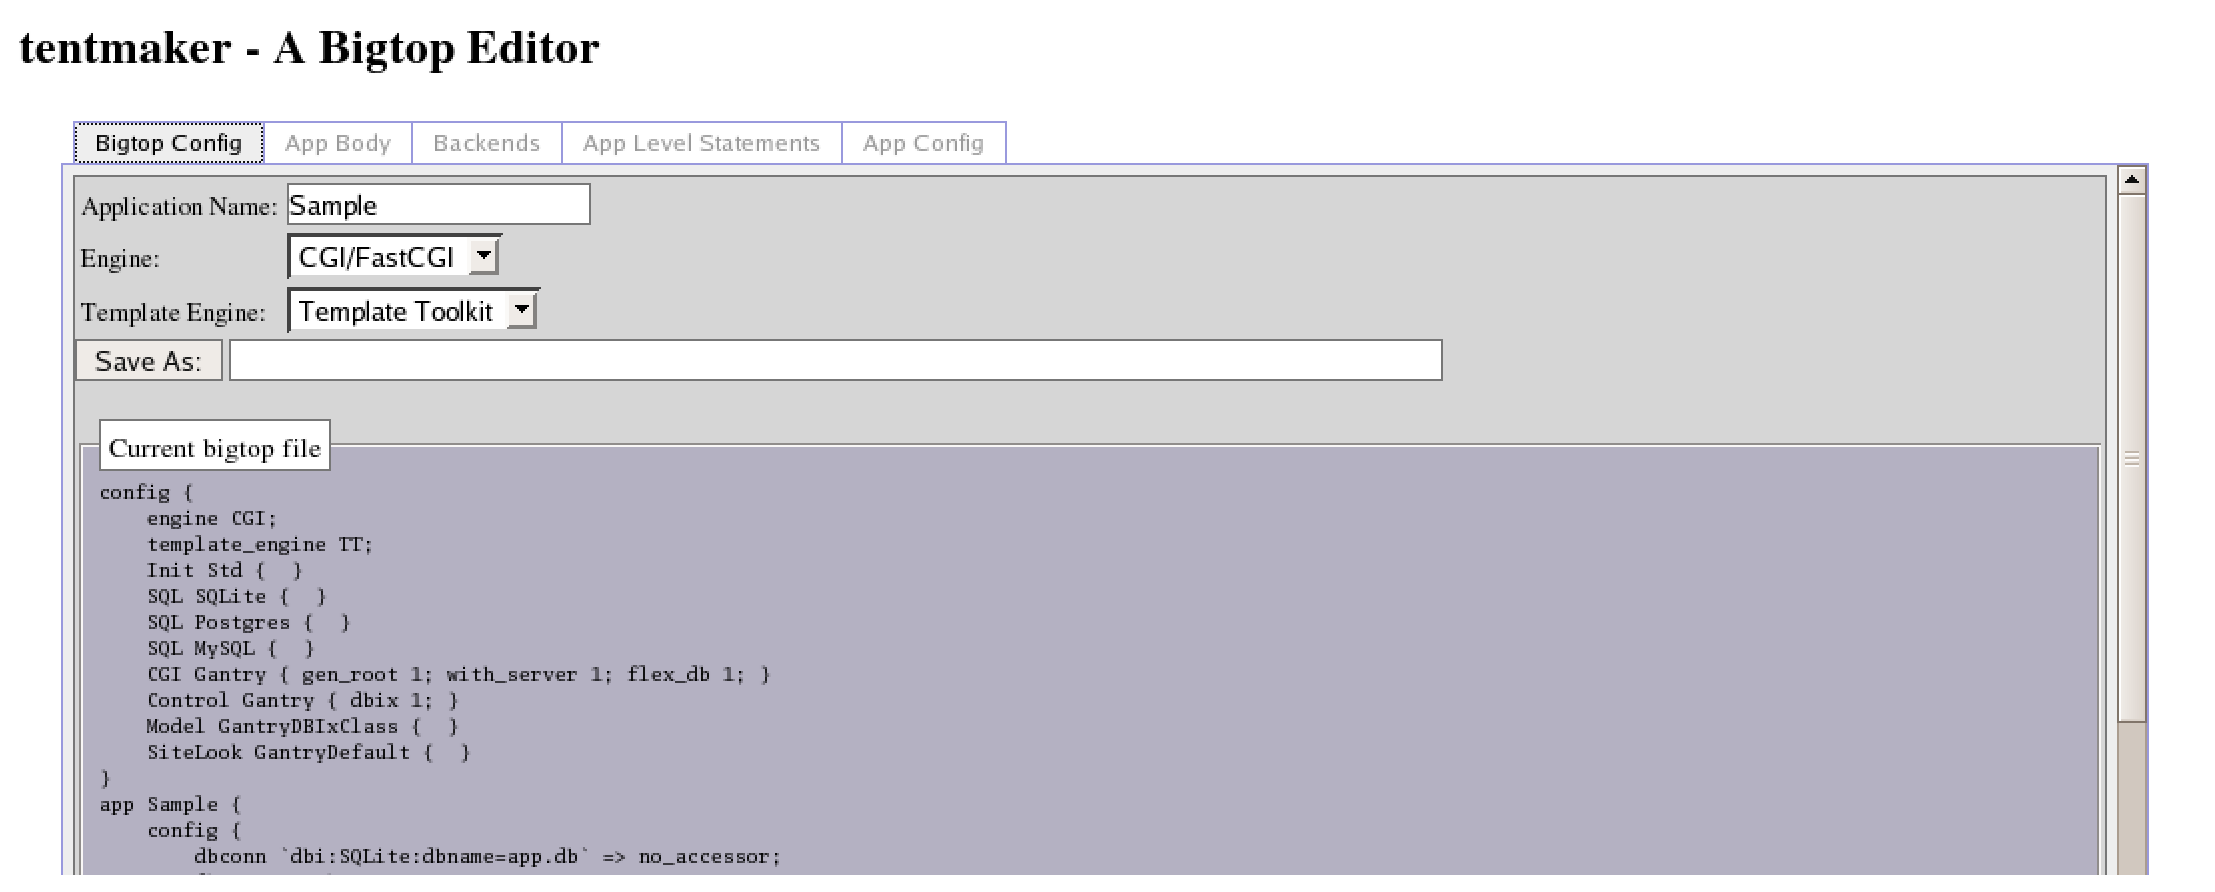
\includegraphics[width=6in]{tentopening}
\caption{The opening appearance of tentmaker.}
\label{fig:tentopening}
\end{figure}

There are five tabs which let you describe your app:

\begin{tabular}{l|l}
Tab Label & Allows you to specify... \\
\hline
Bigtop Config &
    the name of the app and a choice of engines which will serve it \\

App Body &
    the meat of your app, i.e. your tables and controllers \\

Backends &
    the list of all things bigtop should make for you, use check boxes \\
 &  to choose what you want it to do, and input boxes to configure \\
 &  each backend's output \\

App Level Statements &
    author names, their email addresses, project license, etc., all of \\
 &  these have nice defaults \\

App Config &
    a single input table for configuration of your app \\
\end{tabular}

We'll eventually visit all of the tabs in Chapter \ref{chap:tentref},
for now let's concentrate on making our address book work as my wife might
expect.  With that in mind the only thing of current interest on tentmaker's
opening page is the Save As button and the file name next to it.
Once we make our changes, we will return to this tab to press the button.

There are two issues we need to address: the columns in our table and
the database we are using.

To change the column names and add some new ones, click on the `App Body'
tab.  There you will see something similar to Figure \ref{fig:appbody}.

\begin{figure}
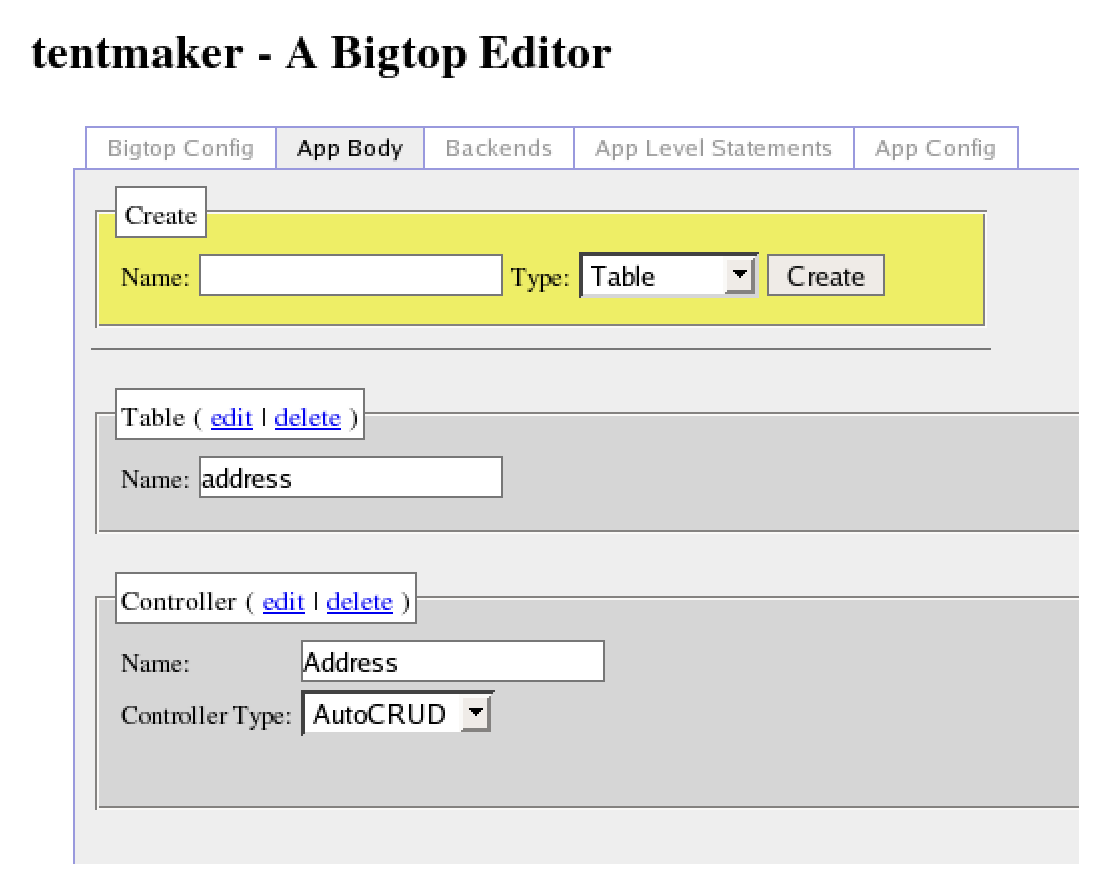
\includegraphics[width=6in]{appbody}
\caption{The App Body tentmaker tab for the address book example.}
\label{fig:appbody}
\end{figure}

We need to change the table and its controller to reflect our column
name preferences.  Start by clicking `edit' for the address table.
This will expand to show the statements and columns defined for the
table, as shown in Figure \ref{fig:tableedit}.

\begin{figure}
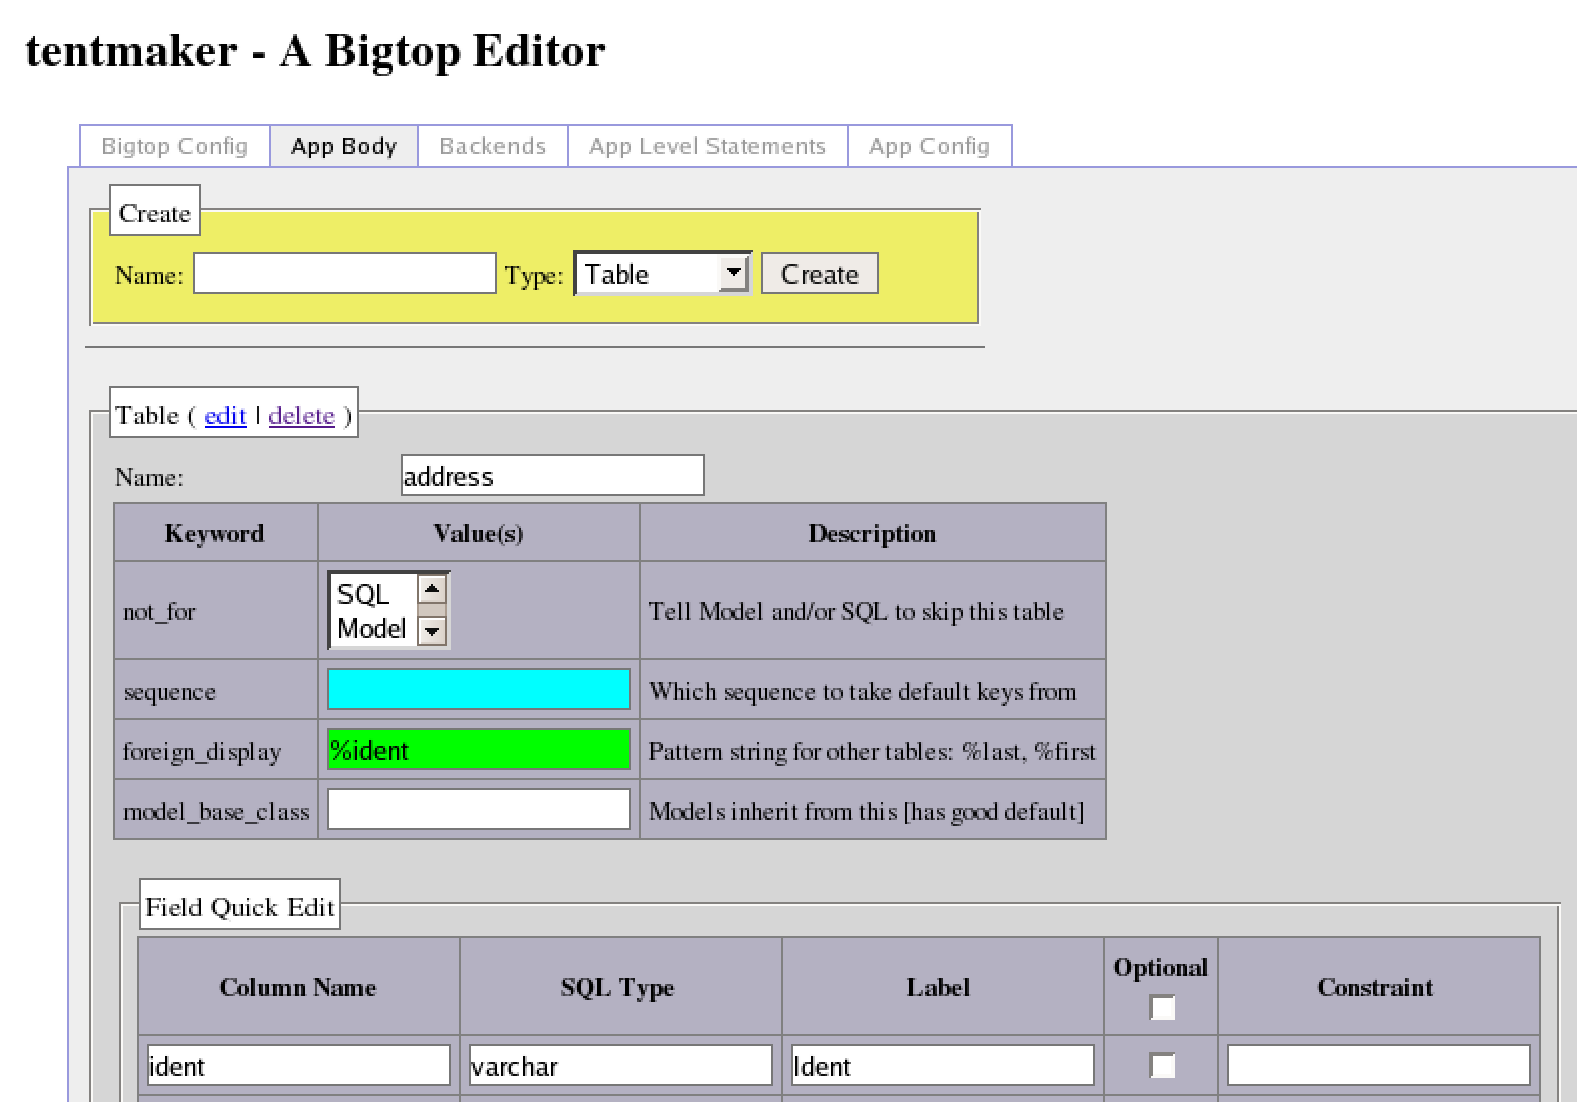
\includegraphics[width=4in]{tableedit}
\caption{Editing a table in tentmaker.}
\label{fig:tableedit}
\end{figure}

You may click edit again, at any time, to collapse the edit box.

First, scroll down in the tabbed pane to the Field Quick Edit
table shown more clearly in Figure \ref{fig:quickedit}.

Our original bigtop generation gave us five columns: id, ident, description,
created, and modified.  The last two are dates in case we want to start
tracking changes.  At least that would give my wife some clue of
address quality.  For now, we'll just ignore those.

The id is a unique primary key assigned by the database.  We can leave
it alone too.  That leaves the dreaded default columns ident and description.
Let's start by changing their names to `name' and `number.'  Just click
into the text fields under the `Column Name' label to do that.  To apply the
changes, click anywhere outside of the input box.  If you can't think
of a better place, feel free to click on the apparently useful
`Apply Quick Edit' button.

This is a good time to add additional fields for address information.
Add these by entering their names into the Create Field box and pressing
the button.  My table has these: address, city, state, zip, and email.
Add any that make sense to you.  Note that you can add as many fields as you
like at once by typing their names, separated by spaces, into the Name(s)
box.

When tentmaker makes a new field for you, it gives it a corresponding
label.  It does that by splitting the name at each underscore
and capitalizing the first letter of each resulting word.
The same things happens when you change the name of a field, if the
old label was formed that way.  If any of those labels looks odd -- perhaps
you prefer `email' to `Email' -- you can change them by typing your choice
into an input box under the `Label' heading.

If the new field should store something more interesting than text, you'll
also need to provide an SQL type for it in the SQL Type column.

Note that there is no reason to change the type from varchar, even if
your database needs something more specific.  The bigtop backend for your
database will magically convert it into something sensible.  If you object
to magic, supply the type of your choice.

Now save the bigtop file and regenerate:

\begin{verbatim}
bigtop docs/addressbook.bigtop all
\end{verbatim}

\subsection*{Dealing with Databases}

Before we restart our app.server, we need to address the database.
The one we used previously will not work, since the app now expects
different column names and more columns.

Since SQLite didn't support table alterations at the time of this writing
(at least not in a production version), we can't keep using the one we
-- or bigtop -- originally built.  This opens the subject of database
support and connection.

For now, we'll rely on the app.server to handle this for us.  See Chapter
\ref{chap:deploy} for how to handle it with CGI/FastCGI or \verb+mod_perl+.

Bigtop supports three databases:
SQLite, Postgres, and MySQL.  Its default generation assumes SQLite,
because it is so easy to work with during initial development.
But its defaults actually make the SQL needed to build the database in
Postgres and MySQL as well.  All of the SQL commands are in the
docs subdirectory of the build directory in files called schema.*,
where the asterisk is replaced with the database name.

If you want to stick with sqlite -- which is the easiest route -- delete
the old app.db, make a new one, and restart app.server:

\begin{verbatim}
sqlite app.db < docs/schema.sqlite
./app.server
\end{verbatim}

For Postgres this process goes like this (adjust the user names and
supply database passwords as needed):

\begin{verbatim}
createdb app.db -U postgres
psql app.db -U regular_user < docs/schema.postgres 
./app.server -d Pg -u regular_user -p password
\end{verbatim}

For MySQL it goes like this (again, adjust the user names and supply
database passwords as needed):

\begin{verbatim}
mysqladmin create app.db -u root -p
mysql -u regular_user -p app.db < docs/schema.mysql
./app.server -d mysql -u regular_user -p password
\end{verbatim}

Regardless of which database engine you use, you can change the name of
the database app.server will use with the -n flag (short for --dbname).

Of course, you could also edit app.server so it uses different defaults.
If you do that, remember to uncheck the `Build Server' box for the
CGI Gantry backend on the `Backends' tab in tentmaker.  Otherwise, whenever
you run bigtop, you changes will be overwritten.

\subsubsection*{Dealing with schema changes}

As development proceeds, data model changes are all but inevitable.
That is really the point of bigtop and its tentmaker editor.  Those
tools help with all the code and schema changes.  But there is one
thing they can't do: alter your database.

Every time I get tool envy about automated schema alterations, my
colleagues talk me out of working on the problem.  They always assert
that they wouldn't trust a tool to make production database alterations
under any circumstances.  Until they change there minds, their probably
won't be a schema change component to bigtop.

But, there is one thing bigtop can do to lessen the pain of data model
changes during development.  You can include literal SQL in the bigtop
file which will go directly into the generated docs/schema.* files
(at present all of them always receive the same SQL).  There is also
a table level data statement.  You can enter as many of these
as you like for any table.  Each one generates an INSERT INTO statement
for its table.  Combining literal SQL with data statements you can
have a nice, fresh database full of all sorts of lovely test data
simply by blowing away your old database and building a new one as shown
above.  Bigtop::Docs::Syntax explains both of these options (searching
there for `literal' or `data' is surprisingly effective).

There are also question/answer pairs about initial data in
Bigtop::Docs::Cookbook.  Look for, `How can I include initial data in a table?'
and `How do I put extra things into schema.*?'

\section{Interlude: Is this really required?}

To make further changes, we can revisit the bigtop file with tentmaker
or a text editor, save the result, and regenerate the app as shown above
(always being careful to alter or replace the database as needed).  For
example, Upon running the new version, I remembered that by default, all
fields are required.  But, Lisa's poor little fingers may not want to type
in all the data for each contact in her book -- she might not even know
most of it for most people.  So, we want to use tentmaker to make the fields
optional on the add and edit form.

Stop the app.server script (if it's still running).  From the build directory,
restart tentmaker, again giving it the existing bigtop file:

\begin{verbatim}
tentmaker docs/addressbook.bigtop
\end{verbatim}

(Remember to provide --port=... if needed.)

Click on the `App Body' tab so we can mark fields as optional in the address
table.  Click on the `address' table's `edit' link.  Lisa wants address,
city, state, zip, phone, and email to be optional (that's right, only name
will be required).  So, we should check the Optional box for
all the fields except name (and possibly phone) in the tentmaker.
We can also do this for all the fields by checking the Optional box in the
heading row.  Then, we can uncheck the ones we want to require, like the
name.

As a final touch, I think it would be a good idea to show the email address
next to the phone number on the main listing.  While still in tentmaker,
scroll down to the controller called Address.  You should see something
like Figure \ref{fig:controledit}.

\begin{figure}
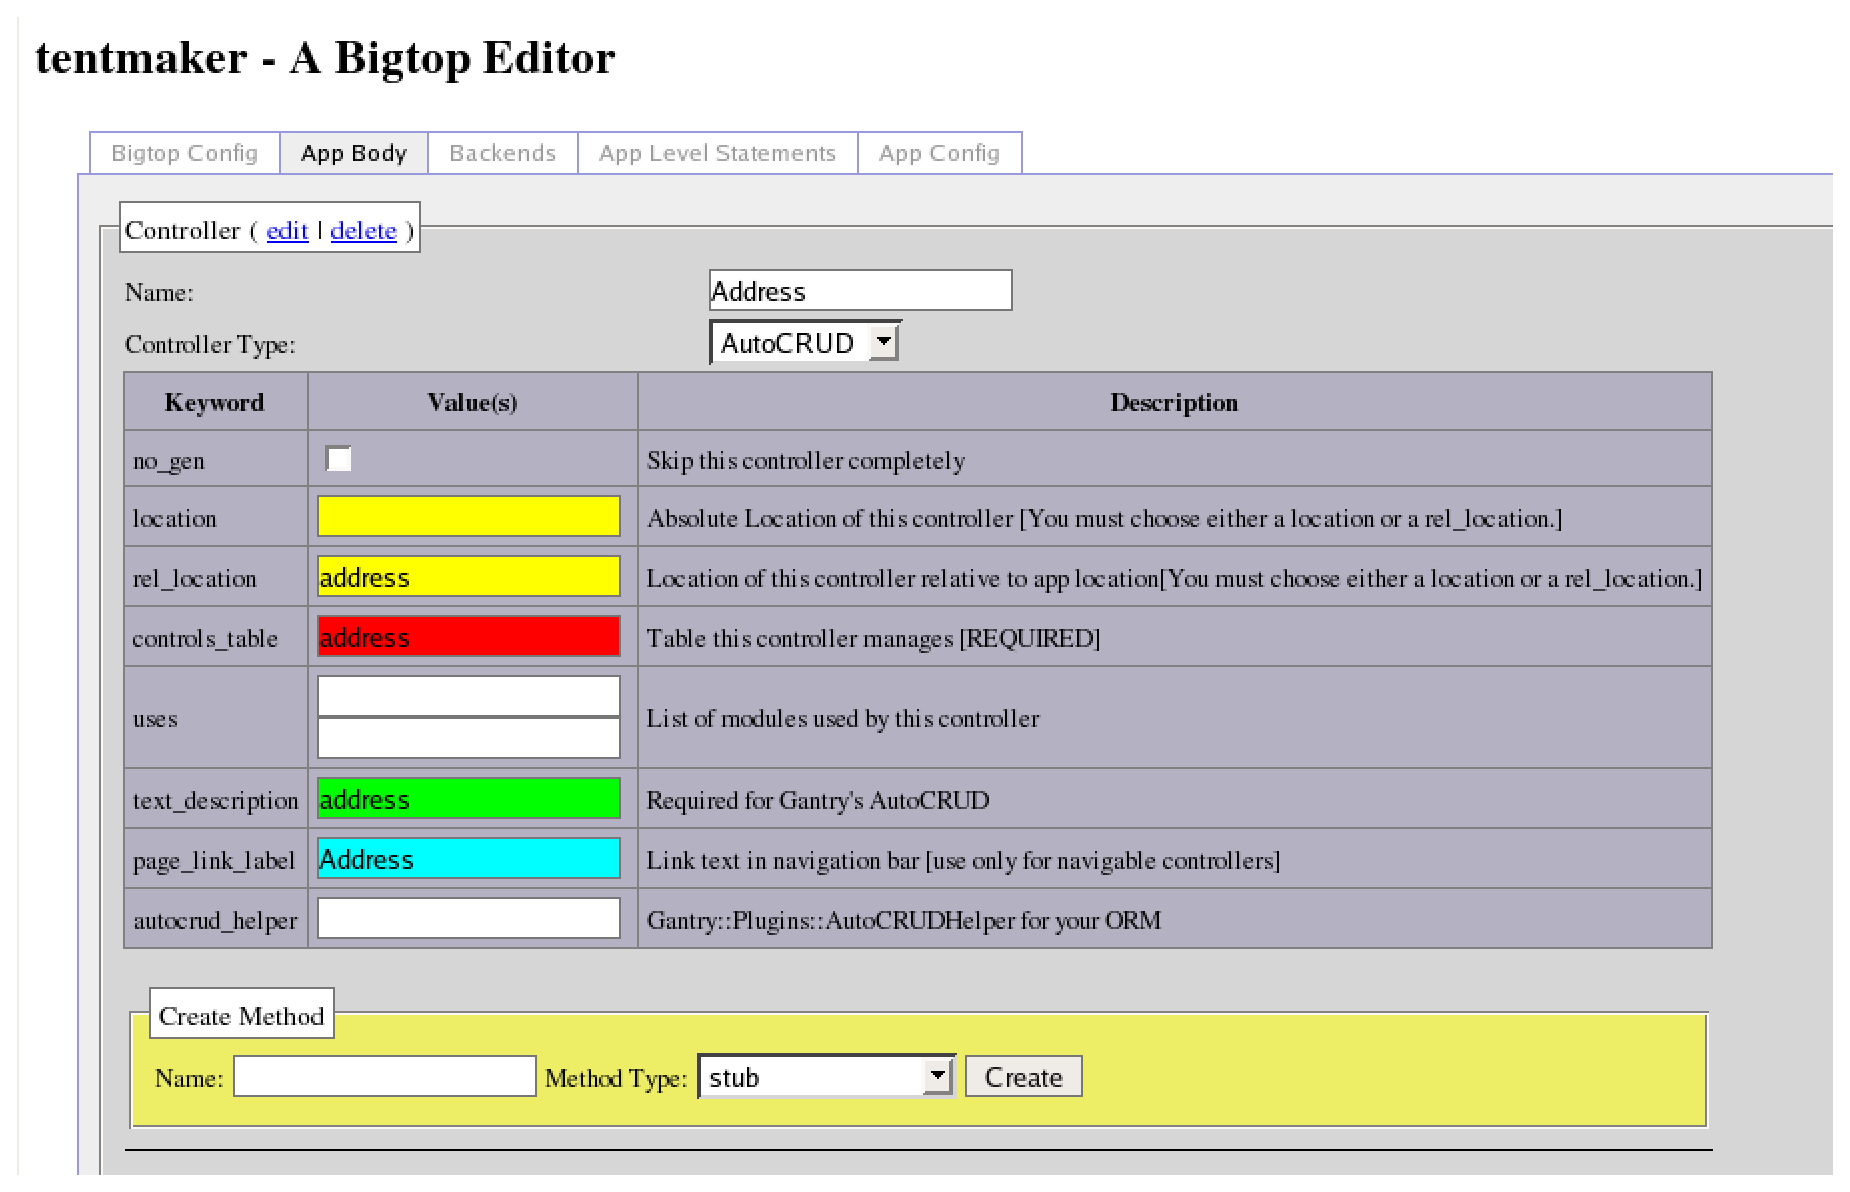
\includegraphics[width=4in]{controledit}
\caption{Editing a table in tentmaker.}
\label{fig:controledit}
\end{figure}

From there look for the method called \verb+do_main+ and edit it as
shown in Figure \ref{fig:mainlistedit}.  Add `email' below `number'
in a \verb+cols+ box.

Save the bigtop file.  Then stop the tentmaker and rebuild the app:

\begin{verbatim}
bigtop docs/addressbook.bigtop all
\end{verbatim}

Since we didn't make changes to the database, we can restart the app
immediately.

\begin{verbatim}
./app.server
\end{verbatim}

(Use whatever command line flags you used before.)

Note that the app.server always looks for your code in the lib subdirectory
of the build directory.  It never looks in blib/lib, so there is no
reason to run Build.PL at this point (unless you want to run the default
tests).

\section{Take Two: Should I send a card?}
\label{sec:asciiart}

Now, let's look at a more interesting exercise in that old address book.
On the back end paper, Lisa has scribbled some birth dates.
Perhaps including those dates in our present app will improve our on-time
arrival percentage for cards and gifts (and then again perhaps not).
It will certainly show off a few features of Gantry and Bigtop.

To add a table, we can ask tentmaker to augment the existing bigtop file
during start up:

\begin{verbatim}
tentmaker -a docs/addressbook.bigtop 'bday->address'
\end{verbatim}

This not only adds the table, but gives it a foreign key pointing to the
address table.  All we need to do from there is change each column name
of the new bday table to something more evocative and make sure they have
the proper `SQL Type.'

Here are all the ASCII art operators and what they mean:

\begin{tabular}{l|l|l}
Operator   & Example & Meaning \\
\hline
\verb+->+  & book->author   & book has a foreign key pointing to author \\
\verb+<-+  & author<-book   & book has a foreign key pointing to author \\
\verb+-+   & user-extrainfo & user and extrainfo have foreign keys to   \\
           &                & each other                                \\
\verb+<->+ & fox<->sock     & fox and sock share a many-to-many relationship\\
\end{tabular}

You can use exactly the same -a flag with bigtop -- and you can use -n
with tentmaker, just like we originally did with bigtop.  Always keep in
mind that using -n or -a with bigtop will automatically rebuild the
application, while tentmaker never rebuilds at all.  Every time you
save your changes in tentmaker, you need to run \verb+bigtop file.bigtop all+
for them to affect the application.

New tables are created in the order they are listed, so \verb+->+ and
\verb+<-+ are synonyms except for the table creation order.

Note that while existing tables mentioned in ASCII art are not recreated,
they will be receive new foreign keys or many-to-many relationships.

With the tentmaker restarted and the new table in place, let's start
by editing the column names for the new bday table, just as we did for
the address table.  Edit the table, change the names of the ident and
description fields.

All that remains is to make the date selectable.  Change the SQL Type of
the birth day field -- whatever you called it -- to date.

After you regenerate the app, there should be a new navigation tab
labeled \verb+Birth Days+ (or some other phrase according to your table name).
Go to it, to start entering birth days.

In this chapter we have seen how to use tentmaker to create a two table
web app for which we didn't have to write any code manually.  The next
chapter explains how to move this app into a \verb+mod_perl+ environment
with or without using Gantry::Conf to manage the configuration information.

Alternatively, now that we have seen how to use tentmaker modify generated
apps, you are ready for a more thorough tour.  If you want to take it now,
go to Chapter \ref{chap:tentref}.
      % using bigtop and tentmaker to make an address book
\chapter{Deployment Issues}
\label{chap:deploy}

% make sure this says something about controlling database connection
% info
% If you want to change to a different database, you can arrange that now.
% Click on the `App Config', you'll see something like Figure
% \ref{fig:appconfig}.
% 
% \begin{figure}
% 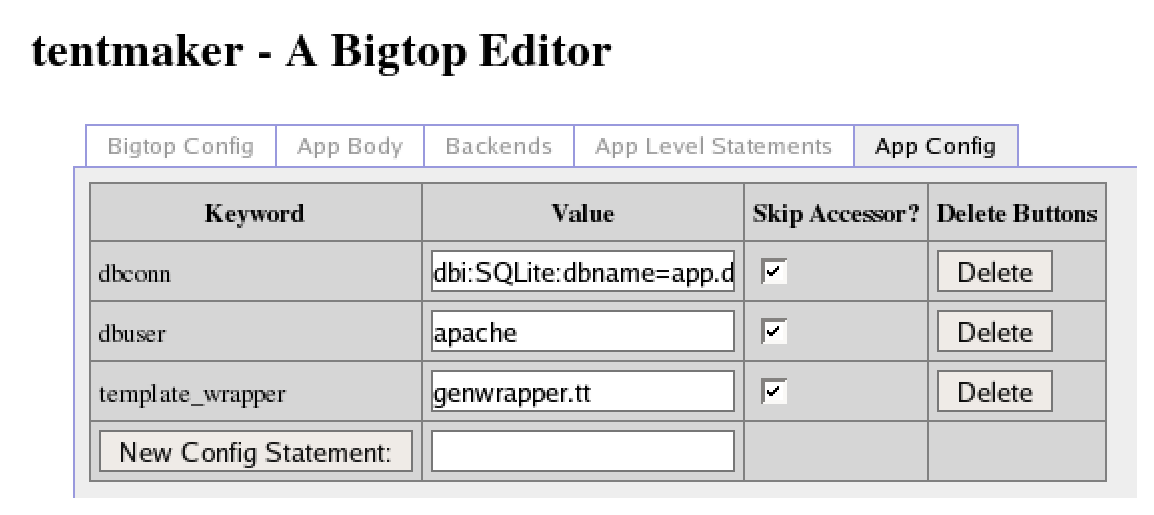
\includegraphics[width=6in]{appconfig}
% \caption{Application configuration table.}
% \label{fig:appconfig}
% \end{figure}
% 
% To change databases, simply change the dbconn config parameter, so it
% has the proper DBI dsn string for connecting to your database.  You probably
% also need to supply a dbuser.  Further, you will need to add a new
% config param called dbpass, if your database expects a password for
% your dbuser.  If so, type `dbpass' into the input box next to the
% `New Config Statement' button, then press the button, and add the password.

In the last chapter, we saw how to build an app with tentmaker and run it
with a test server (app.server).  Bigtop also made a cgi script for us, which
we could immediately deploy merely by moving it to the cgi-bin directory.
Here we will look at two additional deployment issues.  First, we will
move the app into a \verb+mod_perl+ environment.  Second, we will extract the
conf from the app into the Gantry::Conf scheme.  The latter will allow us
to easily deploy multiple instances of our app and share the app's conf info
with external scripts.

\section{Moving to Mod Perl}

I'm not going to explain how to put a working \verb+mod_perl+ installation onto
your server.  But, I am going to explain how to deploy a Gantry app via
\verb+mod_perl+, once you have \verb+mod_perl+ working.

Bigtop can help with much of our work, so begin by restarting the tentmaker
and giving it the contact.bigtop file from the last chapter:

\begin{verbatim}
tentmaker docs/addressbook.bigtop
\end{verbatim}

First -- and foremost -- on the `Bigtop Config' tab, change the engine to
the \verb+mod_perl+ engine you have installed (mine was 1.3 when I wrote this).

Now, click on the `Backends' tab.  Uncheck the box for CGI Gantry, which will
stop bigtop from making app.cgi and app.server.  Then check the box for
HttpdConf Gantry, to start generating docs/httpd.conf.

Since our app is not installed on the system yet, we need to tell
\verb+mod_perl+ where to find it.  A regular \verb+use lib+ statement will do,
but we need to place it carefully.  One good place to put it is at the top
of a $<$Perl$>$ block in httpd.conf.  Here's how to make bigtop do that.

Go to the `App Body' tab.  Create a new block of type `Literal' (leave the
`Name:' box blank).  Scroll down to that block and select `Literal Type:'
`PerlTop.'  This is the instruction telling bigtop to put a statement into
the $<$Perl$>$ block in httpd.conf.  In the `String:' box, type a complete
use lib statement (right down to the semi-colon) which will lead perl to the
blib/lib directory of the build directory.  Mine looks like this:

\begin{verbatim}
use lib '/home/pcrow/AddressBook/lib';
\end{verbatim}

You might even want to include four leading spaces, if you care about the
indentation in the generated conf file.

Now we need to deal with some paths, which were relative for app.server,
but must now be absolute.  While still in tentmaker, go to the `App Config'
tab.  Add a new config variable called \verb+root+.  Make its value
an absolute path to the html directory of the AddressBook build directory.
This directory will need to be readable by the Apache User.

The other path that needs adjustment is for app.db.  For the app to work,
the Apache User needs to own both the app.db file and the directory where
it lives.  In addition to ownership, it obviously needs write permissions.
After you decide where to locate app.db, add a fully qualified absolute path
to it in the `dbconn' value.

Alternatively, you could switch to a different database engine.  Make that
change in the same place, by altering the database connection info string.
Then, don't forget to build the database.  There should be schema files
for use with Postgres and MySQL in the docs directory.

Save the file and regenerate the app:

\begin{verbatim}
bigtop docs/addressbook.bigtop all
\end{verbatim}

There is only one more thing we need to do to launch under \verb+mod_perl+.
We, need to modify the system httpd.conf for our server to tell it about our
app.

For this app, I added the following to my \verb+mod_perl+ enabled httpd.conf:

\begin{verbatim}
<VirtualHost address.devel.example.com>
    ServerName       address.devel.example.com
    DocumentRoot     /home/pcrow/AddressBook/html
    CustomLog        /home/pcrow/logs/combined.log combined
    ErrorLog         /home/pcrow/logs/addressbook.err

    Include /home/pcrow/AddressBook/docs/httpd.conf
</VirtualHost>
\end{verbatim}

You might need to make a DNS entry to use the above approach.  We
have a wild card which lets anything.devel... map to these virtual hosts,
so we can make them on the fly.

Now start or restart the web server and hit the app again at its new URL.

\section{Moving to Gantry::Conf}

The approach to app configuration in the last section and the last chapter
both end up tying the conf info to the app rather tightly.  We want
to move to a more flexible system.  Later subsections will explain two
key example scenarios in which this flexibility is needed: deploying multiple
instances of the same app in the same server and sharing conf info with
external scripts or other apps.

Gantry::Conf was Frank Wiles' idea (he's my boss, do don't be surprised
if I gush in this section).  He was tired of being told by external
app suppliers how he should store his conf info.  He didn't want to do the
same to other people when we deliver an app.  Further, he knew that
our shop was suffering from the difficulty of conf info duplication due
to web apps relying on httpd.conf, while scripts did something different.
This section explains how Gantry::Conf works by showing how to move our
existing AddressBook app to it.

We can turn again to tentmaker to get us started.  Click on `Backends.'
Check the box for Conf Gantry.  Add an instance name for the app in the
box at the far right labeled `Conf Instance.'  I'll call mine \verb+address+.
Then, check the `Use Gantry::Conf' box in the far right hand column in the
HttpdConf Gantry row.  This tells that backend to omit the conf information,
since we are trying to centralize it, not adjust how it is duplicated.
(HttpdConf Gantry will set a variable for the conf instance, and another
for the conf file if that is defined, taking the values from the Conf
Gantry backend).  If you were still using the CGI Gantry backend, you
could do the same thing for it.

Save the file, regenerate with bigtop.  If you restart the server and hit
it now, you will receive an error, because Gantry::Conf does not know where
to find your config.  Copy `AddressBook.gantry.conf' from the docs
directory to the /etc/gantry.d directory, or make a symbolic link.  Make
sure your /etc/gantry.conf has a wild card include:

\begin{verbatim}
include /etc/gantry.d/*.conf
\end{verbatim}

If you can't create or modify /etc/gantry.conf, make a file somewhere which
the Apache User can read.  Put that file's name in the `Conf File' box
in tentmaker for the Conf Gantry backend.  Save and regenerate.
Then, create the master conf file with a wild card like the one shown
above, but pick a directory you can write to and the Apache User can read
from.

Now it is safe to restart the app and point the browser to it.

\subsection{Multiple instances}

One of the key uses of Gantry::Conf is in easing deployment of multiple
instances of the same app.  For instance, if my wife and I each want a
separate address book, we can deploy two instances of the app.  Both will
share some things, like the site appearance and even the database user and
password.  But, they will store data in different databases.  This section
explains how to accomplish this.

First, there is no difficulty in setting up a second virtual server using
the same code.  Just duplicate the VirtualHost shown above and change the
names until it looks more like this:

\begin{verbatim}
<VirtualHost philaddress.devel.example.com>
    ServerName       philaddress.devel.example.com
    DocumentRoot     /home/pcrow/AddressBook/html
    CustomLog        /home/pcrow/logs/combined.log combined
    ErrorLog         /home/pcrow/logs/addressbook.err

    Include /home/pcrow/AddressBook/docs/phil.conf
</VirtualHost>
\end{verbatim}

Notice that I'm letting Lisa keep the original URL, in case she set
a bookmark to it.  Also note that I referred to phil.conf.  I'll have to
copy her conf and update it, but only by changing the GantryConfInstance:

\begin{verbatim}
PerlSetVar GantryConfInstance philaddress
\end{verbatim}

This is slightly painful, since I have to remember to repeat this copy and
change process each time the httpd.conf changes.  (I have a back burner
TODO item to address this.)

With the web server conf updated, I need to correct the conf.  The easiest
way to do that is to again copy the conf, but I want a more robust solution.
I'm going to move the shared conf values into /etc/gantry.conf.  Everything
is shared in this case except the dbconn value, so it will be the lone entry
in each instance's conf file.  Here are the files, starting with
/etc/gantry.conf:

\begin{verbatim}
<shared contact_shared>
    dbuser apache
    template_wrapper genwrapper.tt
    root /home/pcrow/AddressBook/html
</shared>
<instance contact>
    ConfigureVia FlatFile Config::General \
            /home/pcrow/AddressBook/docs/AddressBook.conf
    use contact_shared
</instance>
<instance philcontact>
    use contact_shared
    dbconn dbi:Pg:dbname=philcontact
</instance>
\end{verbatim}

Lisa's instance now wants an individual conf files which has one line:

\begin{verbatim}
dbconn dbi:Pg:dbname=contact
\end{verbatim}

Now when I restart the server, users hitting
\verb+http://contact.devel.example.com/contacts+ will access Lisa's
data.  Users hitting \verb+http://philcontact.devel.example.com/contacts+
will access my data.

There are many other ways to configure the app to work with two instances
using Gantry::Conf.  As with Perl, there is more than one way to do it.
Picking one you like takes a bit of experience.  I've shown a couple of
approaches here to get you started.  Note that all of these have abandoned
conf generation for a manual approach.  One day it may be possible to
generate instance specific conf, but that day has not yet dawned.

\subsection{Sharing conf with batch processes}

Half of the reason for developing Gantry::Conf was to ease the sharing of
conf between the web delivered pieces of an app and its batch processes.
Suppose we want the contact app to spam us with upcoming birthdays.
We can now write a little script to accomplish that and configure it via
the same conf that the app uses.

To show how this works, suppose that I want an email reminder on a periodic
basis (say once a week) of all the birthdays near the the current date.
This would enable me to send cards, if I weren't so mean spirited.

Here is the program which does the job for me:

% /home/pcrow/play/AddressBook/scripts/reminder
\begin{verbatim}
#!/usr/bin/perl
use strict; use warnings;

use lib '/home/pcrow/AddressBook/lib';

use Date::Manip qw( ParseDate DateCalc UnixDate );
use Gantry::Conf;
use AddressBook::Model;
use AddressBook::Model::bday    qw( $BDAY    );

my $instance = shift || 'address';

my $conf = Gantry::Conf->retrieve( { instance => $instance } );

my $schema = AddressBook::Model->connect(
    $conf->{ dbconn }, $conf->{ dbuser }, $conf->{ dbpass },
);

my $today = ParseDate( 'today' );
my $comp_err;

my @bdays = $BDAY->ssearch( $schema );

foreach my $bday_row ( @bdays ) {
    ( my $db_date = $bday_row->bday ) =~ s{-}{/}g;
    my $bday    = ParseDate( $db_date );
    my $name    = $bday_row->name;
    my $family  = $bday_row->address->foreign_display();

    my $separation       = DateCalc( $today, $bday, \$comp_err );
    my ( $weeks, $days ) = ( split /:/, $separation )[2,3];
    my $sign             = substr $separation, 0, 1;

    my $prep = ( $sign eq '+' ) ? 'from now' : 'ago';

    $days += 7 * $weeks;

    my $short_bdate = UnixDate( $bday, "%B %e" );

    if ( abs( $days ) < 14 ) {
            print "$name belonging to $family birth day:\n"
                    .   "   $days days $prep on $short_bdate.\n";
    }
}
\end{verbatim}

The program begins like any other with a shebang line.  Then it uses the
same lib path as the web server, so they will share the code modules.
I wouldn't need the use lib statement, if I had installed the application.

I chose Date::Manip to handle the dates, since it is standard.  From it
I need ParseDate to turn strings into dates, DateCalc to compare dates,
and UnixDate for pretty output.

The rest of the uses bring in the model (and its abbreviation),
Gantry::Conf itself, and a helper which will connect me to my database.

The user supplies the conf instance name at the command line, so Lisa
and I can each receive separate birthday updates.  That instance is
passed to Gantry::Conf's retrieve method, which returns the proper hash
of conf info.

After storing today's date in a Date::Manip string, I ask the bday
table model to return all of its rows.  I could have let the database do
the date work, but chose to do it in Perl in a -- probably vain -- attempt
to be database agnostic.

Looping through each birthday row, I pull out the data I want to use.
Note that I can call \verb+foreign_display+ on the \verb+address+ attribute
of each birth day row, to get the family name from the address table.
This is why we always want a \verb+foreign_display+ for each table.

The rest is just a bit of Date::Manip work and pretty printing.
I'll leave the actual scheduling of the job up to you.  If I really installed
this, I would use cron.  Note that the email is indirect.  The cronned
program prints to standard out, which cron will send to my mail on the local
system.  That's enough for me.  Feel free to add a genuine email feature.

Gantry::Conf is even more flexible than what I've shown here.  Unfortunately,
it is beyond the scope of this book to show more of its details.  For instance,
If I had more room, I could show how to set up a secure conf server which apps
on multiple boxes could contact via https to retrieve shared conf.  Further,
we could explore how to write your own provider, so you could replace flat
file conf with LDAP or some other clever scheme.  Alas, we'll have to turn
away from the fascinating subject of configuration and return to the world
of web apps.  For more information on Gantry::Conf see the perldoc for
Gantry::Conf::FAQ, Gantry::Conf::Tutorial, and the other modules in the
Gantry::Conf namespace.
        % moving to mod_perl an Gantry::Conf
\chapter{Testing}
\label{chap:testing}

When bigtop builds your application, it makes four test files.  These are
kept up to date on each rebuild, unless you turn them off in some way.  This
chapter explains their purposes and uses, then goes on to explain how to
use one of them as a model for building your own more ellaborate tests.

\section{Standard Tests by bigtop}

The Control backends are responsible for building tests to go with their
controllers.  The Control Gantry backend builds and maintains four tests
in the t subdirectory of the build directory:

\begin{tabular}{l|l}
Test Name & Purpose \\
\hline
\verb+01_use.t+      & one \verb+use_ok+ test for each controller stub      \\
\verb+02_pod.t+      & standard Test::Pod \verb+all_pod_files_ok+           \\
\verb+03_podcover.t+ & standard Test::Pod::Coverage \verb+all_pod_files_ok+ \\
\verb+10_run.t+      & default page request for each controller             \\
\end{tabular}

These test files are purposely spartan.  You are not meant to edit them.
To run them, build in the usual way:

\begin{verbatim}
perl Build.PL
./Build
./Build test
\end{verbatim}

Once you do that, you can usually re-run the tests with just the last step.

There is nothing particularly interesting about the \verb+use_ok+ tests,
they merely check compilation of each controller module.  The pod and
pod coverage tests are even less interesting.  To use them, you need to
install Test::Pod and Test::Pod::Coverage and set the \verb+TEST_POD+
environment variable in your shell.

The run tests are slightly more interesting.  There is one test for
each controller in the application, plus one for the base module.  Each
test is a simple page hit on the \verb+do_main+ method, which only checks
for successful return status.  Yet, these can still serve as an example
for your own tests.  So, let's look at them in more detail.

\section{Run Tests}

To explain how to build specific tests, I'll start by walking you through
the tests bigtop makes by default, using \verb+t/10_run.t+ from the
address book example in Chapter \ref{chap:simpleex} in particular.  I'll
show a little bit of the script at a time with comments interspersed.
To see the whole thing simply look at the \verb+t/10_run.t+ bigtop makes
when you type:

\begin{verbatim}
bigtop -n AddressBook address
\end{verbatim}

The real version has a bit more in it.  I've distilled it to show what
you need to do for your own tests, avoiding issues like the SKIP block
which prevents default tests from running if you don't have an SQLite
database for them to use.

The top of the script is typical of any test which relies on Tests::More:

\begin{verbatim}
use strict;

use Test::More tests => 2;

use AddressBook qw{ -Engine=CGI -TemplateEngine=TT };

use Gantry::Server;
use Gantry::Engine::CGI;
\end{verbatim}

It uses the base module of the application, specifying the CGI and TT
engines.  Then it brings in Gantry::Server to drive the tests and the
CGI engine.  The last is used mostly for documentation, since Gantry will
require it based on the import list to AddressBook.

\begin{verbatim}
my $cgi = Gantry::Engine::CGI->new( {
    config => {
        dbconn => 'dbi:SQLite:dbname=app.db',
        template_wrapper => 'genwrapper.tt',
        root => 'html',
    },
    locations => {
        '/' => 'AddressBook',
        '/address' => 'AddressBook::Address',
    },
} );
\end{verbatim}

For testing, we need a CGI engine object.  The configuration here is minimal,
containing only the database DSN string, Template Toolkit wrapper file name,
and trivial root template path.  Recall that the original address book
had only one table called address.  So, there are two locations here: the
base location and one for the sole table.  The locations hash key
stores URL/controller pairs.  The URLs are absolute from the document
root of the server.

\begin{verbatim}
my @tests = qw(
    /
    /address
);
\end{verbatim}

The generated test script will hit each location.  When you write your
own tests, there is no need to repeat these hits on each controller's default
URL.  See Section \ref{sec:customtests} below for how to make more
interesting hits.

\begin{verbatim}
my $server = Gantry::Server->new();
$server->set_engine_object( $cgi );
\end{verbatim}

We need to instantiate a Gantry::Server, which is really an
HTTP::Server::Simple object.  To avoid constructor overloading, Gantry::Server
provides \verb+set_engine_object+.  We pass it the CGI engine object
built earlier.

\begin{verbatim}
foreach my $location ( @tests ) {
    my( $status, $page ) = $server->handle_request_test( $location );
    ok( $status eq '200',
            "expected 200, received $status for $location" );

    if ( $status ne '200' ) {
        print STDERR $page . "\n\n";
    }
}
\end{verbatim}

Gantry::Server provides \verb+handle_request_test+ for testing.  It simulates
a single page request in the application and returns the result.  The
default tests only check the return status.  You could scrape the page
if you so desire.  You could also directly query the database from the
test to see if a particular hit went as expected.  For that you would need
to provide data to the page.  Keep reading.

There are two ways to feed data to a page.  Some pages expect to process
forms, \verb+handle_request_test+ is ready to help them.  It takes anything
from the query string and feeds it as if it were in the body of a POST
request.  For example, suppose you have a controller with location
\verb+/search+, which expects a form parameter called searchstr:

\begin{verbatim}
my @tests = qw(
    /search?searchstr=keyword
);
\end{verbatim}

To understand how to test the rest of the page types, we need to take
a step back and discuss Gantry dispatching.

\section{Gantry Dispatching}

Dispatching is the process of turning a browser requested URL into a method
call.  Gantry has a simple scheme, but there are some subtlies.  

The basic scheme is straightforward.  Whether you deliver the application
with \verb+mod_perl+, CGI, FastCGI, or the stand alone server, you must
specify a list of locations and the controllers which respond to them.  If
the browser requests one of those locations, Gantry will call the
\verb+do_main+ method in the associated controller.

What happens when the requested location is not listed exactly as a location
is more interesting.  Work begins with the full URL.  If that matches
a location, we would be in the basic scheme.  So, one at a time path elements
are removed from the tail of the URL, until what remains is a location from
the list.   The web server does this.  It then passes the remainder of
the URL to Gantry's handler, which uses the first element as the method name
and the remainder as parameters for that method.  Before calling the method,
Gantry prepends \verb+do_+ to the name.  This makes it a bit harder for
URL spoofing to hit methods unexpectedly, but mostly serves as clear
documentation of which methods in a controller are externally visible.

Here's an example.  Suppose that someone requests \verb+/address/meth/a/b+
on our example address book.  The web server (Apache or the stand alone
server) looks for the longest location prefix it can find in its location
list (it finds \verb+/address+) and hands the request to the \verb+handler+
method of the registered module for that location (AddressBook::Address is
registered for \verb+/address+).  The \verb+handler+ method is inherited from
Gantry.pm, which uses the remainder of the url to decide what method to
call.  If nothing were left, it would call \verb+do_main+.  In this case,
\verb+meth/a/b+ remains, so it will call \verb+do_meth+, passing it
\verb+a+ and \verb+b+ as arguments.

\section{Custom Tests}
\label{sec:customtests}

Now that we understand the dispatching scheme explained in the previous
section, it is a small step to creating tests of arbitrary \verb+do_+
methods with parameters and/or form data.

If the method in question is expecting data from the URL, there is not
much to the test.  Simply add it to the URL in the \verb+@tests+ list.
For example:

\begin{verbatim}
my @tests = qw(
    /address/stubby/a/b/c
);
\end{verbatim}

For the current app, this will test a hit to the \verb+do_stubby+ subroutine,
which will receive \verb+a+, \verb+b+, and \verb+c+ as parameters.

%If the method expected its parameters in the query string, we could have said:
%
%\begin{verbatim}
%my @tests = qw(
%    /address/stubby?var=val&var2=val2
%);
%\end{verbatim}

The only thing clever is form submission.  As mentioned above, to post
form parameters, just put them in the query string.  The
\verb+handle_request_test+ method of the Gantry::Server takes the query
string parameters and passes them as if they were POSTed.

Now that you know how to simulate page hits, you can help yourself to the
various Test:: modules on CPAN to complete your custom testing program.
      % the default tests and how to build your own
\part{Case Studies}
\chapter{Contact Us}
\label{chap:contactus}

Suppose your boss asks you to add a 'Contact Us' button on the bottom of the
company web site.  All it should do is display a form with a place for the
customer's email address, a large text box, a submit, and a cancel button.
(Why the boss didn't like your first suggestion of a mailto link is
beyond me.)  Upon submission, the text from the box should go directly into
an email message to \verb+support@example.com+, to be answered sometime in the
next month, if the customer is lucky.

This job is small, but it will show how Gantry can get out of the way when
you have a little bit of non-standard work to do.  I'll still start with
bigtop, but I won't ask it for much help.  After all, there is no database.
So, let's see what we can do with a one controller app, and let's write it
by hand -- at least mostly.

\section{Getting Started}

Even though tentmaker is overkill and bigtop won't be needed to make
code, the latter can still pitch in as a replacement for h2xs in building
the project directory.  To start from scratch without using tentmaker,
type:

\begin{verbatim}
bigtop --new ContactUs
\end{verbatim}

This will work like h2xs, in that it will make a ContactUs subdirectory of
the current directory and put the structure of a CPAN distribution in it.
I like it better than h2xs primarily because it uses Module::Build instead of
ExtUtils::MakeMaker.  It also makes docs/contactus.bigtop in case we do want
to start using tentmaker and/or bigtop to work on the app.

Changing into the ContactUs directory, we are ready to begin hand writting
our app.  The operative code belongs in lib/ContactUs.pm.  Edit that file
and put something like this in it:

\begin{verbatim}
package ContactUs;
use strict;

use base 'Gantry';

sub do_main {
    return "Hi Rob";
}

1;
\end{verbatim}

Saving this will give us a the smallest possible Gantry app, a.k.a.
something to play with.  To deploy this, we could use \verb+mod_perl+,
but it is easier to start with a self standing server.  Here's one:

\begin{verbatim}
#!/usr/bin/perl
use strict;

use Gantry::Server;

use lib 'lib';

use ContactUs qw{ -Engine=CGI -TemplateEngine=Default };

my $cgi = Gantry::Engine::CGI->new();

$cgi->add_location( '/', 'ContactUs' );

my $port   = shift || 8080;
my $server = Gantry::Server->new( $port );

$server->set_engine_object( $cgi );
$server->run();
\end{verbatim}

The key to a self standing server is to use Gantry::Server, which is based
on HTTP::Server::Simple.  The other features of our serving script are:
the use lib statement, which points to the lib directory where our ContactUs.pm
lives; a full use statement for that module, which specifies the CGI engine
and Default templating (which provides no output templating help at all);
constructing a CGI engine object and populating its root location with
our module name; instanstiating the server with a default port of 8080,
which our users can easily override; setting our engine object in that
server; and starting it.

If you start the server at this point and point your browser to it, you
will see a greeting for an old friend of mine.  We still have quite a
bit of work to do in ContactUs.pm, but the server is finished.  In fact,
this server is almost enough for any project.  All you have to do is
add additional \verb+add_location+ calls -- and possibly some
\verb+add_config+ calls.  Bigtop does that for you, but it really isn't
that much work.  (Well, bigtop actually passes all of the config parameters
and location to the CGI engine constructor.)

With our server in good shape, let's make the module perform to spec.

\section{Allowing Them to Contact Us}

There are three things we need to make this application work.  First, we
need a form to take the data.  Second, we need a method to process that
form.  Third, the processing method needs a way to send email.  Let's start
with the form.

Gantry provides Gantry::Utils::HTML for those who don't like templates.
It is in the same spirit as CGI.pm, but the syntax was never meant to match
that venerable module.  Here is the new \verb+do_main+ with the form:

\begin{verbatim}
use Gantry::Utils::HTML qw( :form :table :style );

sub do_main {
    my $self = shift;

    return join '',
        ht_form_js( "$self->{uri}/contactus" ),
            ht_table(),
                ht_tr(),
                    ht_td(), "Your Email Address:", ht_utd(),
                    ht_td(), ht_input( 'email',   'text' ), ht_utd(),
                ht_utr(),
                ht_tr(),
                    ht_td(), "What We Need to Know:", ht_utd(),
                    ht_td(),
                        ht_input( 'message', 'textarea', '',
                                  'rows="12" cols="75"' ),
                    ht_utd(),
                ht_utr(),
            ht_utable(),
            ht_submit( 'Submit', 'Submit' ),
            ht_submit( 'Cancel', 'Cancel' ),
        ht_uform;
}
\end{verbatim}

All of the methods in the HTML utility module return lists of strings.  The
main Gantry handler is expecting a single string, hence I used join to
build a single string from the various lists.

To start the form, I called \verb+ht_form_js+, giving it the URL which
will process the form (it is handled by \verb+do_contact_us+ below).
To finish it, I called \verb+ht_uform+.  In the middle, I used other
methods to make a rudimentary input form, laid out as a table.

The two input items are in the table with labels on the left and entry widgets
on the right.  Below that table are the submit and cancel buttons.

Alternatively, I could have hand coded the HTML in my controller, but that
is even uglier.  Most of us would prefer to use a template, but there are
plenty of examples of that approach in other parts of this book.

Processing the form is fairly straighforward.  We need a method with the
same name as the POST action of the form with the \verb+do_+ prefix.  For
my example, the method name is \verb+do_contactus+.  If the task was more
complicated, that same URL could even map to the \verb+do_main+ of a different
controller.

Here is the shell of the form processor:

\begin{verbatim}
sub do_contactus {
    my $self = shift;

    my $params = $self->get_param_hash();

    return ht_h( 2, 'Thank you for contacting us.' );
}
\end{verbatim}

This method has the three essential steps of a Gantry form handler: (1)
it takes the site object as it invocant, (2) it requests the form
parameters by calling \verb+get_param_hash+, (3) it returns something.
Sometimes the return value is a redirection to a better place in the
app.  This one is a dead end thank you.

If you are using Template Toolkit, substitute returning something from
the handler for passing the template name to the template accessor and
putting data for the template into a hash inside the stash:

\begin{verbatim}
$self->template( 'mytemplate.tt' );
$self->stash->controller->data( $data_hash_ref );
\end{verbatim}

All that remains is to send the mail.  You can use your favorite mailer
to do that; mine is Mail::Sendmail.  So, my first version looks like this:

\begin{verbatim}
sub do_contactus {
    my $self = shift;

    my $params = $self->get_param_hash();

    sendmail(
        To      => 'support@example.com',
        From    => 'contactus@example.com',
        Subject => "Contact Us Message from $params->{ email }",
        Message => $params->{ message },
        smtp    => 'smtp.example.com'
    ) or warn "couldn't send $params->{ message } to support\@example.com";

    return ht_h( 2, 'Thank you for contacting us.' );
}
\end{verbatim}

I'm depending on my mailer to sanatize any tainted data that the user
might have submitted.

Even though I like whitespace and very pretty layout, this app is only
48 lines of code, counting the \verb+1;+ at the bottom -- but not counting
its docs.

\section{Playing Well with our Sysadmin}

We really should do one more thing.  We should allow the system administrator
to control who gets the mail and which SMTP server it goes through.  For this,
we should create a conf instance like this in our \verb+/etc/gantry.conf+:

\begin{verbatim}
<instance contactus>
    contactus_email   support@example.com
    contactus_from    contactus@example.com
    smtp_host         smtp.example.com
</instance>
\end{verbatim}

Then we need to tell the serving script that we want to use this instance.
This requires adding \verb+use Gantry::Conf;+ to the top of the script and
this link immediately after \verb+add_location+:

\begin{verbatim}
$cgi->add_config( 'GantryConfInstance', 'contactus' );
\end{verbatim}

Now, all that remains is to use the config variables in the
\verb+do_contactus+ method.  Here is the new version:

\begin{verbatim}
sub do_contactus {
    my $self = shift;

    my $params = $self->get_param_hash();

    sendmail(
        To      => $self->fish_config( 'contactus_email' ),
        From    => $self->fish_config( 'contactus_from' ),
        Subject => "Contact Us Message from $params->{ email }",
        Message => $params->{ message },
        smtp    => $self->fish_config( 'smtp_host' ),
    ) or warn "couldn't send $params->{ message } to support\@example.com";

    return ht_h( 2, 'Thank you for contacting us.' );
}
\end{verbatim}

Now our sysadmin can control the mail flow from conf.  In particular, this
allows development and production systems to send to different addresses
via different smtp hosts.

While I don't write many apps by hand from start to finish, Gantry can help
you do that, right down to hiding the uglier aspects of HTML even while
you include it in the controller.  We've seen all the pieces you need to
write such slender apps in this case study.  We will now return to a lazier
way.
     % web form, no database
\chapter{Billing Customers}
\label{chap:billingapp}

This example is adapted from the first working Gantry app that did anything
useful.  It was written by Tim Keefer to track his consulting invoices
and appears in a slightly modified form in Bigtop::Docs::Tutorial.  The
version here is very similar to the one in that document, but I've
updated it to our current notions of best practices.

If you are like me, you work for a paycheck.  Perhaps once or twice a year
you do some side work that needs an invoice.  If so, you might do what I
do and type that invoice into a text editor and send it via email.  The
date on the email and a quick check of bank deposits is enough to track it.
But, if you have a few more side jobs, manual invoicing starts to break down.
Hence our case study for this chapter: a billing system for occasional
consultants or landlords with a few tenents who owe them for utilities.

For the purposes of discussion, for the rest of the chapter, I'll pretend
to be a high powered consultant who has too many clients to track by hand.

\section{A Billing Data Model}

As I asserted in Chapter \ref{chap:simpleex}, most web apps are database
front ends.  Our billing app will be no different.  So, let's begin
with the data model.  There are five tables:

\begin{tabular}{l|l}
Table Name          & Purpose                                             \\
\hline
\verb+customers+    & People who occasionally owe me money                \\
\verb+my_companies+ & Names I call myself when doing business             \\
\verb+invoices+     & Bills customers receive in email and eventually pay \\
\verb+line_items+   & Tasks listed on invoices                            \\
\verb+status+       & A code table describing invoice statuses
\end{tabular}

Figure \ref{fig:billing_model} shows all the fields in these tables, but
it was made long ago.  Some of the field names have been changed to
reflect better practices.  This mostly affects the foreign keys.

\begin{figure}
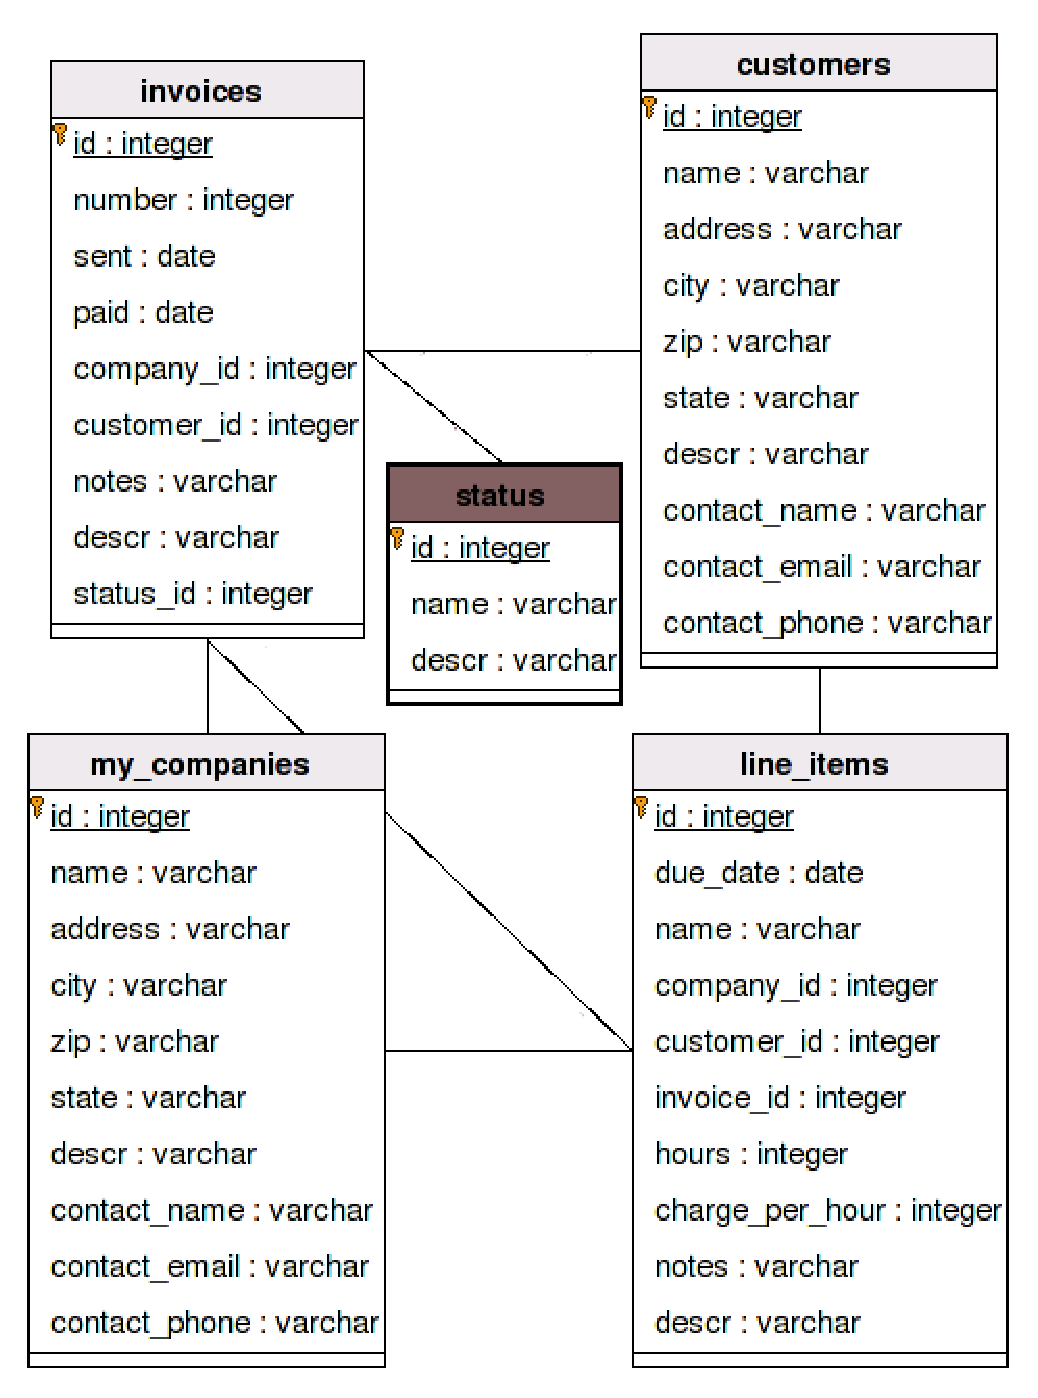
\includegraphics[height=6in]{billing_model}
\caption{Original billing application data model.}
\label{fig:billing_model}
\end{figure}

\section{Bigtop File for Billing App}

While I could walk you through using bigtop and tentmaker to build this
data model, that wouldn't add much to previous chapters, see for example
Chapter \ref{chap:simpleex}.  Instead, I'll show you the finished bigtop
file I made with bigtop, tentmaker, and my favorite editor.  While tentmaker
is great for getting started, it is often easier to move to a text editor to
fill in large chunks of repetitive descriptions.  Here is the finished result,
over 300 lines of it:

\begin{verbatim}
config {
    engine          CGI;
    template_engine TT;
    Init            Std             {}
    CGI             Gantry          { with_server 1; gen_root 1; flex_db 1; }
    SQL             Postgres        {}
    SQL             MySQL           {}
    SQL             SQLite          {}
    Control         Gantry          { dbix 1; }
    Model           GantryDBIxClass {}
    SiteLook        GantryDefault   {}
}
app Billing {
    authors `Phil Crow`, `Tim Keefer`;
    config {
        dbconn           `dbi:SLQite:dbname=app.db` => no_accessor;
        template_wrapper `genwrapper.tt`  => no_accessor;
    }
    table    my_company      {
        foreign_display `%name`;

        field id { is int4, primary_key, auto; }
        field name {
            is             varchar;
            label          Name;
            html_form_type text;
        }
        field address {
            is             varchar;
            label          Address;
            html_form_type text;
        }
        field city {
            is             varchar;
            label          City;
            html_form_type text;
        }
        field state {
            is             varchar;
            label          State;
            html_form_type text;
        }
        field zip {
            is             varchar;
            label          Zip;
            html_form_type text;
        }
        field description {
            is                 varchar;
            label              Description;
            html_form_type     text;
            html_form_optional 1;
        }
        field contact_name  {
            is                 varchar;
            label              `Contact Name`;
            html_form_type     text;
        }
        field contact_email {
            is                 varchar;
            label              `Contact Email`;
            html_form_type     text;
        }
        field contact_phone {
            is                 varchar;
            label              `Contact Phone`;
            html_form_type     text;
        }
        data
            name => `Crow Motors`,
            address => `12 E. Main`,
            city => `Paxton`,
            state => `NE`,
            zip => 69155,
            description => `Car and Implement Sales and Service`,
            contact_name => `EJ`,
            contact_email => `ej@example.com`,
            contact_phone => `1-800-CROW-MOT`;
    }
    table    customer         {
        foreign_display `%name`;

        field id { is int4, primary_key, auto; }
        field name {
            is             varchar;
            label          Name;
            html_form_type text;
        }
        field address {
            is             varchar;
            label          Address;
            html_form_type text;
        }
        field city {
            is             varchar;
            label          City;
            html_form_type text;
        }
        field state {
            is             varchar;
            label          State;
            html_form_type text;
        }
        field zip {
            is             varchar;
            label          Zip;
            html_form_type text;
        }
        field description {
            is                 varchar;
            label              Description;
            html_form_type     text;
            html_form_optional 1;
        }
        field contact_name  {
            is                 varchar;
            label              `Contact Name`;
            html_form_type     text;
            html_form_optional 1;
        }
        field contact_email {
            is                 varchar;
            label              `Contact Email`;
            html_form_type     text;
            html_form_optional 1;
        }
        field contact_phone {
            is                 varchar;
            label              `Contact Phone`;
            html_form_type     text;
            html_form_optional 1;
        }
        data
            name => `Groover Nordqvist`,
            address => `502 E. Third`,
            city => `Paxton`,
            state => `NE`,
            zip => 69155,
            description => `Prime Customer`,
            contact_name => `Groover`,
            contact_email => `gnordqvist@example.com`,
            contact_phone => `Unlisted`;
    }
    table    line_item        {
        foreign_display `%name`;

        field id { is int4, primary_key, auto; }
        field due_date {
            is               date;
            label            `Due Date`;
            date_select_text Select;
            html_form_type   text;
        }
        field name {
            is               varchar;
            label            Name;
            html_form_type   text;
        }
        field invoice {
            is                 int4;
            label              `Invoice Number`;
            refers_to          invoice;
            html_form_type     select;
        }
        field hours {
            is                 int4;
            label              Hours;
            html_form_type     text;
        }
        field charge_per_hour {
            is                 int4;
            label              Rate;
            html_form_type     text;
        }
        field notes {
            is                 text;
            label              `Notes to Customer`;
            html_form_type     textarea;
            html_form_optional 1;
            html_form_rows     4;
            html_form_cols     50;
        }
        field description {
            is                 text;
            label              `Notes to Self`;
            html_form_type     textarea;
            html_form_optional 1;
            html_form_rows     4;
            html_form_cols     50;
        }
    }
    table    invoice          {
        foreign_display `%number`;

        field id { is int4, primary_key, auto; }
        field number {
            is                 varchar;
            label              Number;
            html_form_type     text;
        }
        field status {
            is                 int4;
            label              Status;
            refers_to          status;
            html_form_type     select;
        }
        field sent {
            is                 date;
            label              `Sent On`;
            date_select_text   `Popup Calendar`;
            html_form_type     text;
            html_form_optional 1;
        }
        field paid {
            is                 date;
            label              `Paid On`;
            date_select_text   `Popup Calendar`;
            html_form_type     text;
            html_form_optional 1;
        }
        field my_company {
            is                 int4;
            label              `My Company`;
            refers_to          my_company;
            html_form_type     select;
        }
        field customer {
            is                 int4;
            label              Customer;
            refers_to          customer;
            html_form_type     select;
        }
        field notes {
            is                 text;
            label              `Notes to Customer`;
            html_form_type     textarea;
            html_form_optional 1;
            html_form_rows     4;
            html_form_cols     50;
        }
        field description {
            is                 text;
            label              `Notes to Self`;
            html_form_type     textarea;
            html_form_optional 1;
            html_form_rows     4;
            html_form_cols     50;
        }
    }
    table    status            {
        foreign_display `%name: %description`;

        field id { is int4, primary_key, auto; }
        field name {
            is             varchar;
            label          Name;
            html_form_type text;
        }
        field description {
            is             varchar;
            label          Description;
            html_form_type text;
        }

        data name => `Working`, description => `Work in Progress, NOT Billed`;
        data name => `Sent`,    description => `Mailed to Customer`;
        data name => `Paid`,    description => `Payment Received`;
    }
    controller Status is AutoCRUD {
        controls_table   status;
        rel_location     status;
        text_description status;
        page_link_label  Status;
        method do_main is main_listing {
            title            `Status`;
            cols             name;
            header_options   Add;
            row_options      Edit, Delete;
        }
        method form is AutoCRUD_form {
            form_name        status;
            fields           name, description;
            extra_keys
                legend     => `$self->path_info =~ /edit/i ? 'Edit' : 'Add'`;
        }
    }
    controller Company is AutoCRUD {
        controls_table   my_company;
        rel_location     company;
        text_description company;
        page_link_label  Companies;
        method do_main is main_listing {
            title            `My Companies`;
            cols             name, contact_phone;
            header_options   Add;
            row_options      Edit, Delete;
        }
        method form is AutoCRUD_form {
            form_name        company;
            all_fields_but   id;
            extra_keys
                legend     => `$self->path_info =~ /edit/i ? 'Edit' : 'Add'`;
        }
    }
    controller Customer is AutoCRUD {
        controls_table   customer;
        rel_location     customer;
        text_description customer;
        page_link_label  Customers;
        method do_main is main_listing {
            title            `Customers`;
            cols             name, contact_name, contact_phone;
            header_options   Add;
            row_options      Edit, Delete;
        }
        method form is AutoCRUD_form {
            form_name        customer;
            all_fields_but   id;
            extra_keys
                legend     => `$self->path_info =~ /edit/i ? 'Edit' : 'Add'`;
        }
    }
    controller LineItem is AutoCRUD {
        controls_table   line_item;
        rel_location     lineitem;
        uses             Gantry::Plugins::Calendar;
        text_description `line item`;
        page_link_label  `Line Items`;
        method do_main is main_listing {
            title            `Line Items`;
            cols             name, due_date;
            header_options   Add;
            row_options      Edit, Delete;
        }
        method form is AutoCRUD_form {
            form_name        line_item;
            all_fields_but   id;
            extra_keys
                legend     => `$self->path_info =~ /edit/i ? 'Edit' : 'Add'`,
                javascript => `$self->calendar_month_js( 'line_item' )`;
        }
    }
    controller Invoice is AutoCRUD {
        controls_table   invoice;
        rel_location     invoice;
        uses             Gantry::Plugins::Calendar;
        text_description invoice;
        page_link_label  Invoices;
        method do_pdf   is stub {
            extra_args   `$id`;
        }
        method do_main is main_listing {
            title            `Invoices`;
            cols             number, customer, status;
            header_options   Add;
            row_options
                Tasks => `"/lineitem/main/$id"`, PDF, Edit, Delete;
        }
        method form is AutoCRUD_form {
            form_name        invoice;
            all_fields_but   id;
            extra_keys
                legend     => `$self->path_info =~ /edit/i ? 'Edit' : 'Add'`,
                javascript => `$self->calendar_month_js( 'invoice' )`;
        }
    }
}
\end{verbatim}

There is one notable feature of this bigtop file. The \verb+status+,
+\verb+customer+ and \verb+my_company+ tables use data statements.  In
\verb+status+ they provide the actual data for the table.  Users will be
able to add, edit, and delete in the table, but these are meant to be
useable as a production starting point.  The other two use data statements
to supply test data.  This softens the blow of discarding a database during
development.  Normally I would remove the data statements before building
the final schema files.  But even when I forget, the pain is limited to
deleting two rows from the production database.

You cannot currently manage data statements with tentmaker.  But it will
not alter the ones you put in with an editor, except to cannocalize whitespace.
Each data statement begins with \verb+data+, then has a comma separated
list of field name/value pairs, where the field names and values are separated
by \verb+=>+.  The values must be properly quoted.  The statement ends with
a semi-colon.  You may use as many data statements as you like.
Each one becomes a separate INSERT INTO statement.

Turning the above into a working app is as simple as the example in Chapter
\ref{chap:simpleex}:

\begin{verbatim}
bigtop --create billing.bigtop all
cd Apps-Billing
sqlite app.db < docs/schema.sqlite
./app.server
\end{verbatim}

\section{Finishing the Bills}

Of course, the app so far is generic.  It does not know how to make PDF
invoices or even how to display the tasks associated with an invoice, but
it does all the other tedious parts.

So, let's finish it.  There are only a few remaining pieces, both start in
the Invoice controller.

\subsection*{Showing Tasks for One Invoice}

First, let's link invoices to their tasks.  From the bigtop file in the
previous section, you can see that the generated row option for Tasks points
to the Line Item controller:

\begin{verbatim}
        options => [
            {
                text => 'Tasks',
                link => "/lineitem/main/$id",
            },
        #...
\end{verbatim}

The idea is to call the \verb+do_main+ in the Line Item controller, passing
it the invoice number, to which it should limit the line items displayed.
For that to work, we need to modify the \verb+do_main+ Bigtop generated
for us.  The generated one is almost right.  So, I copied it from
GEN/LineItem.pm to LineItem.pm.  There is no need to modify the bigtop file
or remove it from the GEN module.  Stub controllers inherit from their
generated modules, so we can simply override the method.

In order for my new \verb+do_main+ method to work, I need to use a couple
of additional modules at the top of the \verb+LineItem+ controller:

\begin{verbatim}
use Billing::Model::line_item qw( $LINE_ITEM );
use Billing::Model::invoice   qw( $INVOICE   );
\end{verbatim}

Actually, the first of those was already present, but I removed some
whitespace to make it prettier.

Here is the new \verb+do_main+, lines marked with # * are new, those
with M are modified:

\begin{verbatim}
#-----------------------------------------------------------------
# $self->do_main( [ $invoice_id ] )                                 # M
#-----------------------------------------------------------------
sub do_main {
    my ( $self, $invoice_id ) = @_;                                 # M

    my $only_one_invoice = 0;                                       # *
    my $title            = 'Line Items';                            # *
    if ( defined $invoice_id ) {                                    # *
        $only_one_invoice = 1;                                      # *
        my $invoice = $INVOICE->gfind( $self, $invoice_id );        # *
        $title .= ' for Invoice ' . $invoice->foreign_display();    # *
    }                                                               # *

    $self->stash->view->template( 'results.tt' );
    $self->stash->view->title( $title );

    my $retval = {
        headings       => [
            'Name',
            'Due Date',
            'Invoice',
        ],
        header_options => [
            {
                text => 'Add',
                link => $self->location() . "/add",
            },
        ],
    };

    my $schema = $self->get_schema();
    my @rows   = $LINE_ITEM->get_listing( { schema => $schema } );

    ROW:                                                            # *
    foreach my $row ( @rows ) {
        my $id = $row->id;

        next ROW if ( $only_one_invoice and $id != $invoice_id );   # *

        push(
            @{ $retval->{rows} }, {
                data => [
                    $row->name,
                    $row->due_date,
                    $row->invoice->foreign_display(),
                ],
                options => [
                    {
                        text => 'Edit',
                        link => $self->location() . "/edit/$id",
                    },
                    {
                        text => 'Delete',
                        link => $self->location() . "/delete/$id",
                    },
                ],
            }
        );
    }

    $self->stash->view->data( $retval );
} # END do_main
\end{verbatim}

The main changes are at the top.  First, I altered the opening commit to
show future coders that invoice id is an optional parameter.   Then, inside
the sub, I check the value.  If it is true, I set a flag, get the invoice
with that id, and append its name to the title.

I made only two other changes: I gave the line item walking loop a label
and I added a test which skips rows for other invoices, if we care.  Remember
that users may hit the page directly.  Then they presumably want to see
all the tasks.

\subsection*{How Many Tasks Must I Do?}

For shear fun, I decided that the Tasks link should indicate how many
tasks are associated with the invoice.  While this is clearly not necessary,
it does show some addtional techniques, further I've done it for other apps
to the delight of my users.

This change also involves overriding \verb+do_main+, but less dramatically.
The new Invoice.pm \verb+do_main+ dispatches to the parent version in the
GEN module, then modifies it:

\begin{verbatim}
#-----------------------------------------------------------------
# $self->do_main(  )
#-----------------------------------------------------------------
sub do_main {
    my $self = shift;

    $self->SUPER::do_main();

    my $rows             = $self->stash->view->data()->{ rows };
    my $line_item_counts = $LINE_ITEM->get_count( $self );

    foreach my $row ( @{ $rows } ) {
        my $task_option = $row->{ options }[0];
        my $id          = ( split /\//, $task_option->{ link } )[-1];
        my $count       = $line_item_counts->{ $id } || 0;
        $task_option->{ text } .= " ($count)";
    }
}
\end{verbatim}

When the SUPER version finishes, the template data is in
\verb+$self->stash->view->data()+.  In particular, we are interested in the
\verb+rows+ hash key.  For each row, we want to add a count of tasks after
the link text `Tasks'.  First, we need to know how many tasks there are for
this invoice.  The neatest way to find out is to ask the model.  Later we
will see how it calculates these counts.  For now, it is enough to know
that they come back in a hash reference keyed by invoice row id.

Once we have the data from the parent (GEN) module and a count of all the
tasks collated by invoice, we are ready to walk through the output rows.
Each row is itself a hash.  One key, the one we care about, is `options.'
It stores the links and locations for the right hand column.  Users click
these to navigate.  Usually there are only Edit and Delete links.  Recall
from above that this app also has Tasks and PDF.

The Tasks link comes first (element zero in the array).  We are interested
in the text, but we must retrieve the row id from the link.  That id is
the last element of the URL, hence the split on slashes using only the item
at index -1.  With the id, we can look up the task count for the invoice.
Finally, we can append the the count (in parentheses) to the link text.

The remaining piece counts the tasks, grouping them by invoice id.  It is
implemented in a method in the model stub.  Thus, the following code goes
in \verb+lib/Billing/Model/line_item.pm+:

\begin{verbatim}
sub get_count {
    my $class       = shift;
    my $gantry_site = shift;

    my %retval;

    my @line_items = $class->gsearch( $gantry_site );

    foreach my $line_item ( @line_items ) {
        $retval{ $line_item->invoice->id }++;
    }

    return \%retval;
}
\end{verbatim}

Gantry's DBIx::Class model base class provides \verb+gsearch+ and other
helper methods to save some typing.  This one does a search on the table.
Since no args were provided beyond the site object (which knows how to
get the schema), all rows are returned.

A quick loop through the line items collects the counts in a hash, which
is returned as a hash reference.

\subsection*{Printable Invoices}

With a realitively easy way for users to examine task/invoice connections,
it is time to actually make invoices.  The full version that ships with
Bigtop has a PDF generator in it.  I'm leaving that out here, because it
is large and repetative.  Instead, I'm going to make a plain text invoice.
It won't look as nice, but it will save almost a hundred lines of code
(most of those lines are PDF positioning statements).  Even so, these routines
are rather large and are largely uninteresting.

So that the link structure will not break, I'm still calling the method
\verb+do_pdf+.  Feel free to change the links, etc.

\begin{verbatim}
#-----------------------------------------------------------------
# $self->do_pdf( $id )
#-----------------------------------------------------------------
sub do_pdf {
    my ( $self, $id ) = @_;

    # pull variables out of invoice row ready for here doc
    my $invoice     = $INVOICE->gfind( $self, $id );
    my $invoice_num = $invoice->number;
    my $sent        = $invoice->sent;
    my $description = $invoice->description || '';

    $description    = "\n$description\n" if $description;

    # my company data
    my %corp_data;

    foreach my $column qw( name address city state zip contact_phone ) {
        $corp_data{ $column } = $invoice->my_company->$column();
    }

    # customer data
    my %cust_data;
    foreach my $column
            qw( name address city state zip contact_phone contact_name )
    {
        $cust_data{ $column } = $invoice->customer->$column();
    }

    # tasks, pass the buck
    my ( $task_output, $total ) = $self->_task_output( $id );

    my $retval = << "EO_Invoice";
Billed By:
$corp_data{ name }
$corp_data{ address }
$corp_data{ city }, $corp_data{ state } $corp_data{ zip }
$corp_data{ contact_phone }

Billed To:
$cust_data{ name }
$cust_data{ address }
$cust_data{ city }, $cust_data{ state } $cust_data{ zip }
$cust_data{ contact_phone }
Attn: $cust_data{ contact_name }

Invoice Number: $invoice_num Invoice Date: $sent $description

Date         Hours    Rate/hr    Total   Task
$task_output
_______________________________________________________________________

Total Amount Due: $total

Invoice due upon receipt.
EO_Invoice

    $self->template_disable( 1 ); 		# turn off templating
    $self->content_type( 'text/plain' );

    return $retval;
}
\end{verbatim}

This generates all of the output except the actual task list, which is below.
First, I retrieve the invoice to be made printable, using the \verb+gfind+
method provided by Gantry's DBIx::Class base module.  From it I fish out
various strings to go on the bill.  I want to fish first instead of trying
to call methods inside the here doc.

Then, I fish the company and customer data from the invoice row object.
Once the data is fished out, it is a simple matter of here doc construction.
The tasks are presented via their own method:

\begin{verbatim}
sub _task_output {
    my ( $self, $id ) = @_;

    my @tasks = $LINE_ITEM->gsearch( $self, { invoice => $id } );

    my @rows;
    my $total       = 0;
    my $space       = ' ';

    foreach my $task ( @tasks ) {
        my $row_amount = $task->hours() * $task->charge_per_hour();

        $total        += $row_amount;

        my $row_output = $task->due_date()        . $space x 4;
        $row_output   .= $task->hours()           . $space x 8;
        $row_output   .= $task->charge_per_hour() . $space x 9;
        $row_output   .= $row_amount              . $space x 10;
        $row_output   .= $task->name();

        push @rows, $row_output;
    }
    my $task_output = join "\n", @rows;
    
    return $task_output, $total;
}
\end{verbatim}

Since each task will go on one line, the fishing can be done directly into
the output.  Note that the cost of each line item is calculated here and
a total is returned along with the text for each line item.

Now, when the user clicks Tasks on the invoice page, they will go to the
Line Item controller, but see only the tasks for that invoice.  When the
user clicks PDF, they will get a new page with the text ready for inclusion
in a sickly looking email.  The genuine PDF version looks a bit better.

Keep in mind that all preceding code was written for programmer efficiency
only.  Most of the code could be written to minimize other costs, like
run time.  If the app is successful, expect to be required to make such
changes over time.  But, I always start with getting something that works,
which is easy to read.  Only after a speed problem emerges do I shift from
optimizing for my time to optimizing for the computer's time.

In this chapter, we have seen how to customize a Bigtop generated app with
a minimum of new code  While that may not be the best use a computer's
time for large apps, it is quite a good use of our time for most apps.

The next chapter presents another case study beginning with Bigtop and ending
with custom code.  This time, concepts such as Apache basic auth and
many-to-many relationships between tables appear.
    % original billing app
\chapter{Job Ads}
\label{chap:jobads}

Suppose that our company web site will soon feature a new set of job ads.
The old way of typing directly into html pages has worn through.  In this
chapter, we'll build the foundation for the new system, by creating a web
app to enter and update job and position descriptions.  [Our shop actually
feeds job ads to our public facing web server via RSS from an internal
Gantry bulletin board app.]

The key features of the application from a pedogogical point of view are
these: many-to-many relationships between database tables, limiting who
can access the app (auth), and creative CRUD where a single page submission
leads to activity in multiple tables.

\section{Step One: Creating Jobs and Their Skills}

Eventually the powers that be want a complete on-line way to manage job
descriptions, position announcements, and to track applications for those
positions.

While the plans for the app are ambitious, we are starting modestly,
with three main concepts: job descriptions, skills, and positions.  Each
of these will be a table in the database, but we need one more.  Since
the relationship between skills and job descriptions is many-to-many, we
need a table to join them.

A job description will have a title and a general description, like
``Cleaner'' - ``Keeps the building sparkling.''  There could be quite
a few people with that job description, each one is in a position.
But, for our purposes we will use `position' as short hand for `position
announcement.'  These let the world know that we are looking to expand our
fast-paced, team-oriented environment with a number of highly motivated
self-starters.  Skills are things that people are able to do, like
``coffee making.''  But we will probably stretch the term skill to
include things like ``valid driver's license and clean driving record.''

We're ready to write the vast bulk of the app.  Let's start with
tentmaker:

\begin{verbatim}
tentmaker -n JobAd 'job<->skill position->job'
\end{verbatim}

With the structure in place, use tentmaker to make the normal changes.
To begin, change the name of the ident field in the job table to `title.'
For once, `description' can stay as is.  Then, add fields for
travel percent, on site, and time percent.

The last two new fields will require the user to choose from a list of
options.  In the last chapter we had a similar problem with the invoice
status.  There, I chose to use a table to specify the statuses.  We
could do the same here.  But, in the interest of diverse solutions (and to
save data model complexity), let's let the app front end control the choices.

Start by choosing \verb+on_site+ from the `Edit Field:' selection
list.  That will reveal form elements which control all aspects of the
field and should look something like Figure \ref{fig:fieldedit1}.

\begin{figure}
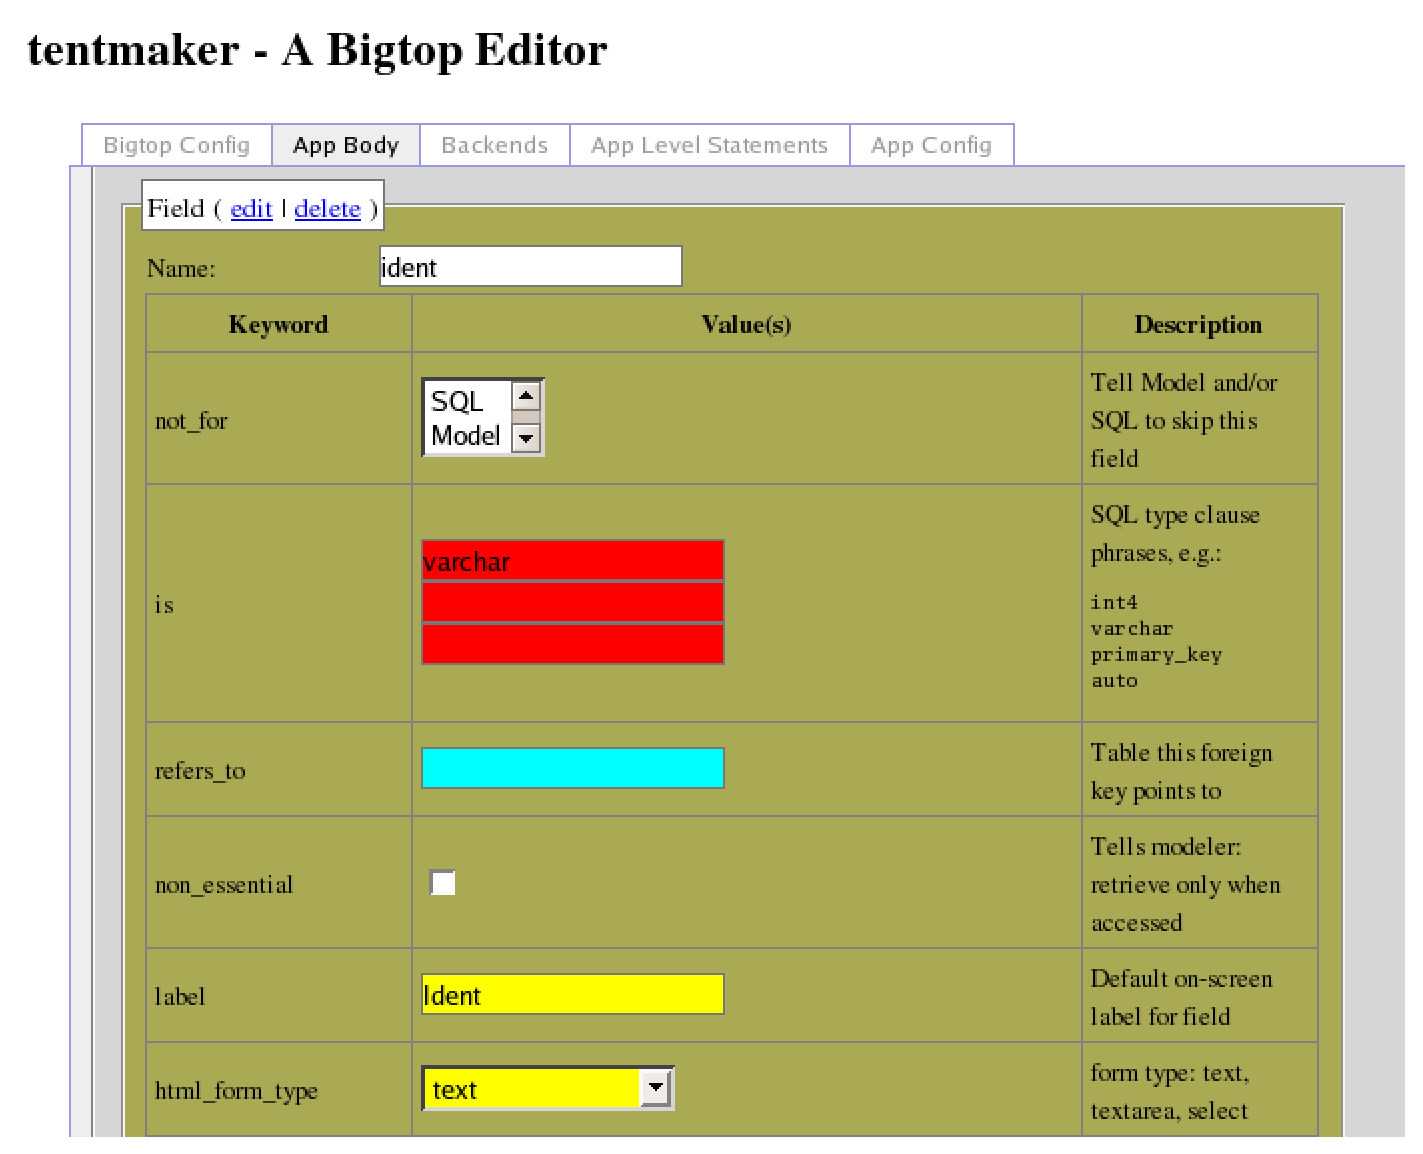
\includegraphics[width=6in]{fieldedit}
\caption{Full field edit form (same as Figure \ref{fig:fieldedit}).}
\label{fig:fieldedit}
\end{figure}

Some of these are represented in the quick edit table, but not
the ones we need to set.  First, choose `select' from the
\verb+html_form_type+ drop down menu.  Then, scroll down until you see
\verb+html_form_options+.  Enter the following:

\begin{tabular}{l|l}
Label               & Database Value    \\
\hline
On-Site             & onsite            \\
Partial Telecommute & parttele          \\
Telecommute         & tele              \\
\end{tabular}

Do the same things for \verb+time_percent+.  First, choose
\verb+html_form_type+ select.  Then, enter options like these:

\begin{tabular}{l|l}
Label               & Database Value    \\
\hline
Full Time           & fulltime          \\
Part Time           & parttime          \\
Contract            & contract          \\
\end{tabular}

This technique gives us data integrity, so long as all database access
is through the app.  But it saves us two tables in this case.

That's all we need to do for the job table.  The skill table is the rare
bird which can use the default fields.  So, let's edit the position
table.  The position description will be formed from the job description
and skills list, so we should delete that field.  To delete a field,
first select it from the `Edit Field:' drop down.  Then click delete
in the legend of the field set that surrounds the full edit form.
Finally, click `Ok' in response to `Are you sure you want to delete' in
the confirmation pop-up.  (Deleting is one thing that is always easier
in a text editor, but switching back and forth can itself be tedious.)

We need to add fields to this table.  Mine are called \verb+n_openings+,
\verb+location+, \verb+closes+, \verb+boss+, and \verb+pay+.  Only two
of them need more work.  Make the SQL Type for \verb+closes+ `date.'
Then make the SQL Type for \verb+n_openings+ int4 and add a constraint to
it: \verb_qr{^\d+$}_.  This will make sure the number is positive.  Well,
it does allow zero, feel free to craft a better regex.

This is enough to put in the job descriptions, the position announcements,
and the skills.  But it doesn't provide a way to link the skills to their
job descriptions.  And, as we'll see later, it doesn't meet management's
full requirement set.  It will serve as our starting point, so save the
bigtop file and stop tentmaker.

Since we didn't start with bigtop in new mode, we need to do the initial
build of the app:

\begin{verbatim}
bigtop -c jobad.bigtop all
\end{verbatim}

This creates the build directory JobAd, which you should change to.
You could spell out -c as --create.  Now, it is probably a good idea to
edit the bigtop file in \verb+docs/jobad.bigtop+ so that its Init Std
config block looks like this:

\begin{verbatim}
    Init Std { no_gen 1; }
\end{verbatim}

In new mode, bigtop does this for us.  It tells bigtop not to build any
of the Init Std files.  These include MANIFEST, which would be safe to
update.  But they also include Change, which should remain, well unchanged.
You could also be more specific, picking the files you want to leave alone:

\begin{verbatim}
    Init Std { Changes no_gen; }
\end{verbatim}

You could also make those choices on the `Backends' tab in tentmaker.
Finally, we are ready to begin customizing the application, starting
with initial user objections.

\section{Authorizing Users}

Upon seeing the original data model from the last section, management
immediately asked us to track logged in users and what they did to the data.
This is a two fold request.  First, have a login scheme so only certain
people can access the app.  Second, when they are in the app, track what
they do in a change log.  This section tackles the first request, the next
section the second.

There are many ways to authorize users in a web app.  Gantry, can help you
do it, if you choose to use Apache basic auth.  This section explains how
to accept that help.  Always remember that Gantry is here to help you, if
you don't feel it is helping, it will gladly step out of the way.  When you
do use Gantry's auth scheme, you should run your server over SSL, keep it
behind a firewall, or both.

To understand Gantry's auth scheme, you need to understand a bit about
how our business uses Gantry.  We deliever many applications via the
web.  Most of them are served to employees behind our firewall.  Therefore,
we want all the apps to use the same user names and passwords.  In fact,
we only want to store those once.  So, we have a master auth database
where everyone's login credentials are stored.  Ideally, each app uses
it for validation.  In reality there are exceptions, with some apps
periodically pulling updates from master auth into their own auth tables.
Here, I will focus on the ideal.  Thus, there will be two databases:
jobad.db and auth.db.  The second can easily be shared across an
organization's apps (we even share ours with apps written with the
prior version of Gantry, which never left the shop).  I must admit that
this approach also simplifies the following discussion.  It is harder to
use Gantry's auth scheme when the auth tables are embedded in the app's
database, not impossible, just harder.

To create your auth database, use a schema file that comes in the
gantry distribution: docs/authschema.sql (Postgres) or docs/authschema.sqlite.
As we will see below, Gantry provides controllers for maintaining the
data in the database once you build it.

Here is a tour of the auth data model.  The key table is \verb+auth_users+.
It has the user name, real name, and password for each user.  The other
tables are tied to it in one way or another.

In addition to individual rights, many apps, including this one, have group
requirements.  Suppose that any valid user may update or add job descriptions
and skills, but only HR can create and manage positions.  This leads to one
group: HR.  In addition, we might want an admin group to manage the
\verb+auth_users+ table.  For now the HR group members will be allowed to
do that.  Gantry auth uses \verb+auth_groups+ to name the groups and
\verb+auth_group_members+ to enroll users in them.  There is also an ip based
auth scheme, but we don't need to think about that for this app.

We don't need to add tables or controllers to our bigtop file for the
auth scheme, but we do need to add some conf to make it happen.  First,
I'll use \verb+mod_perl+.  You could also use CGI, but not the stand alone
server, which does not understand the HTTP auth protocol.





This is enough to put in the job descriptions, the position announcements,
and the skills.  But it doesn't provide a way to link the skills to their
job descriptions.  And, as we're about to see, it doesn't meet management's
full requirement set.

This bigtop file assumes that you are going to incorporate the auth tables
into your app's regular database.  But, you could change that simply by
altering the DBI connection string for \verb+auth_dbconn+ in the app level
config block.

The best way to set up the auth part of your database is to use the schema
provided in the docs directory of the Gantry distribution, though that will
take a bit of translation if you don't use Postgres.

Once you have the database set up, you can easily turn on location based
auth by user or group in your apache conf.

\section{Tracking User Changes}

\begin{verbatim}
changelog
    id
    user_id
    descr
\end{verbatim}

%\begin{figure}
%\includegraphics[width=6in]{name}
%\caption{Caption.}
%\label{fig:name}
%\end{figure}
     % job ad management with AJAX
\part{Gantry Reference}
        %\chapter{A Peek Under the Hood}
\label{chap:gantrytour}

Having seen one simple app in several incarnations, you might be wondering
exactly what Gantry is doing.  This chapter is a sneak peek into what files
bigtop made and how Gantry uses those, plus its own code, to make our app
runs.

\section{The Files}

This section will give you a tour of the files bigtop has been making and
remaking for us.  You probably noticed a few of these like README, Build.PL,
etc.  Those are not particularly interesting.  Here, I'll walk you through
the ones that do real work.  There is one section for each relevant file,
other files are similar to the ones discussed.

\subsection*{app.server}

This is the file you were executing in Chapter \ref{chap:simpleex}:

\begin{verbatim}
#!/usr/bin/perl
use strict;

use lib qw( blib/lib lib );

use Contact qw{ -Engine=CGI -TemplateEngine=TT };

use Gantry::Server;

use Gantry::Engine::CGI;

my $cgi = Gantry::Engine::CGI->new( {
    config => {
        dbconn => 'dbi:Pg:dbname=contact',
        dbuser => 'apache',
        template_wrapper => 'genwrapper.tt',
        root => '/home/pcrow/Contact/html:/home/pcrow/srcgantry/root',
    },
    locations => {
        '/' => 'Contact',
        '/contacts' => 'Contact::Contact',
        '/bday' => 'Contact::BDay',
    },
} );

my $port = shift || 8080;

my $server = Gantry::Server->new( $port );
$server->set_engine_object( $cgi );
$server->run();
\end{verbatim}

The use lib makes sure that the server can find the code modules whether
you use ./Build or not.  But once you use it, you must keep using it, since
it looks in blib/lib first.  Any changes to lib files will not be noticed
once they appear in blib/lib.

Gantry has a stand alone server called Gantry::Server.  It is based on
HTTP::Server::Simple and relies on the CGI engine -- but that doesn't mean
that it forks a process for each request, it is persistent, it just uses
the CGI engine to handle requests.

The CGI engine expects a hash reference with two subhashes, one for config
and the other for locations.  Each location is a url suffix the user can
hit via the server.  If you use Gantry::Conf, you can replace the whole config
subhash with:
\begin{verbatim}
config => { GantryConfInstance => 'contact' }
\end{verbatim}
You may also add the optional GantryConfFile key if you don't use
\verb+/etc/gantry.conf+  See Chapter \ref{chap:deploy} for more details
on Gantry::Conf.  See the section on the CGI Gantry bigtop backend
in Chapter \ref{chap:backends} for instructions on how to set up Gantry::Conf
for app.server and CGI environments via tentmaker.

The server uses port 8080 by default, but accepts an overriding port number
from the command line.  The Gantry::Server constructor is inherited
from HTTP::Server::Simple, so a call to \verb+set_engine_object+ is needed
to load it with our CGI object.  The \verb+run+ method is also supplied
by HTTP::Server::Simple.  A little later we'll look at what happens inside that
method.

\subsection*{Contact.pm}

For small apps the base module is mostly a waste of space.  For larger apps,
it becomes home to common code.  Since the contact app is of the small
veriety, there is not much of interest in Contact.pm:

\begin{verbatim}
package Contact;

use strict;

our $VERSION = '0.01';

use base 'Gantry';

use Contact::Contact;
use Contact::BDay;

##-----------------------------------------------------------------
## $self->init( $r )
##-----------------------------------------------------------------
#sub init {
#    my ( $self, $r ) = @_;
#
#    # process SUPER's init code
#    $self->SUPER::init( $r );
#
#} # END init

1;

=head1 NAME

Contact - the base module of this web app

#... More POD ...
\end{verbatim}

To begin, it is a documentation placeholder.  It explicitly uses the modules
in the app -- at least the ones it knew about when it was written.

There is also a potentially useful init method provided as a comment.
Uncomment it if you need to handle config info that Gantry doesn't know about.
For instance, to handle an SMTP host for genuine emailing, you could use
this init and accessor pair:

\begin{verbatim}
sub init {
    my ( $self, $r ) = @_;

    # process SUPER's init code
    $self->SUPER::init( $r );

    $self->smtp_host_set( $self->fish_config( 'smtp_host' ) );

} # END init

sub smtp_host_set {
    my ( $self, $value )   = @_;
    $self->{__SMTP_HOST__} = $value;
}

sub smtp_host {
    my ( $self ) = @_;
    return $self->{__SMTP_HOST__};
}
\end{verbatim}

By calling \verb+fish_config+, we allow Gantry to use Gantry::Conf if
the app is deployed with it, or a fall back scheme if it is not.  Which
fall back scheme will be determined by the engine.  This is one important
part of engine independence, allowing us to move easily between CGI and
\verb+mod_perl+ for instance.

Again, since all other modules in the app (except the models) inherit
from this package, it is a good place to locate common code.

\subsection*{Contact/Contact.pm}

The controller stub for the contact table looks like this:

\begin{verbatim}
package Contact::Contact;

use strict;

use base 'Contact';
use Contact::GEN::Contact qw(
    do_main
    form
);

use Gantry::Plugins::AutoCRUD qw(
    do_add
    do_edit
    do_delete
    form_name
);

use Contact::Model::contact qw(
    $CONTACT
);

#-----------------------------------------------------------------
# $self->do_main(  )
#-----------------------------------------------------------------
# This method supplied by Contact::GEN::Contact

#-----------------------------------------------------------------
# $self->form( $row )
#-----------------------------------------------------------------
# This method supplied by Contact::GEN::Contact


#-----------------------------------------------------------------
# get_model_name( )
#-----------------------------------------------------------------
sub get_model_name {
    return $CONTACT;
}

#-----------------------------------------------------------------
# text_descr( )
#-----------------------------------------------------------------
sub text_descr     {
    return 'contact';
}

1;

... POD ...
\end{verbatim}

I call this a stub for the obvious reason that it starts empty, except
for use statements.  You might not ever have to put any code here (in
which you could promote the next piece to its place).  But, as with the
base module for the whole app, we often need some special code
for our pages.  This is where it goes.

Otherwise, this is another documentation place holder.  It is meant to be
very easy for someone to open this file and see exactly what it does, even
if there is almost no code.  This is why it has so many comments and
why it explicitly imports everything it uses.

\subsection*{Contact/GEN/Contact.pm}

The real code that manages the contact table is here:

\begin{verbatim}
# NEVER EDIT this file.  It was generated and will be overwritten without
# notice upon regeneration of this application.  You have been warned.
package Contact::GEN::Contact;

use strict;

use base 'Exporter';

our @EXPORT = qw(
    do_main
    form
);

use Contact::Model::contact qw(
    $CONTACT
);

#-----------------------------------------------------------------
# $self->do_main(  )
#-----------------------------------------------------------------
sub do_main {
    my ( $self ) = @_;

    $self->stash->view->template( 'results.tt' );
    $self->stash->view->title( 'Contacts' );

    my $retval = {
        headings       => [
            'Name',
            'Phone',
            'Email',
        ],
        header_options => [
            {
                text => 'Add',
                link => $self->location() . "/add",
            },
        ],
    };

    my @rows = $CONTACT->get_listing();

    foreach my $row ( @rows ) {
        my $id = $row->id;
        push(
            @{ $retval->{rows} }, {
                data => [
                    $row->name,
                    $row->phone,
                    $row->email,
                ],
                options => [
                    {
                        text => 'Edit',
                        link => $self->location() . "/edit/$id",
                    },
                    {
                        text => 'Delete',
                        link => $self->location() . "/delete/$id",
                    },
                ],
            }
        );
    }

    $self->stash->view->data( $retval );
} # END do_main

#-----------------------------------------------------------------
# $self->form( $row )
#-----------------------------------------------------------------
sub form {
    my ( $self, $row ) = @_;

    my $selections = $CONTACT->get_form_selections();

    return {
        name       => '',
        row        => $row,
        fields     => [
            {
                name => 'name',
                label => 'Name',
                type => 'text',
                is => 'varchar',
            },
            {
                name => 'phone',
                optional => 1,
                label => 'Phone',
                type => 'text',
                is => 'varchar',
            },
            {
                name => 'street',
                optional => 1,
                label => 'Street',
                type => 'text',
                is => 'varchar',
            },
            # ... other similar hashes
        ],
    };
} # END form

1;

#... POD ...
\end{verbatim}

The \verb+do_main+ method we created with tentmaker is shown in all its
glory here.  Its purpose is to draw data from the underlying table
and feed it to the standard \verb+results.tt+ template.  That template expects
a hash reference with these keys: \verb+headings+, \verb+header_options+,
and \verb+rows+.  The headings are column labels, the header options usually
just lists Add, which allows users to add rows to the table.  Other options
would likely be reports.  The rows are the data for the table.

The rows are an array of hashes with \verb+data+ and \verb+options+ keys.
The data is just an array of the values from the underlying table.  The
options are things that can be done to the row like Edit or Delete.
Note that the urls of the options are specified (in terms of the location
of the invocant).

When the data structure is ready, it is placed into the stash's view data.

The \verb+form+ method first asks the model for any foreign keys the
user might be allowed to choose.  They go unused here, but come in to
play for the BDay controller.  It requires users to choose a contact family
for each birthday row.

The method builds a hash reference for use by the \verb+form.tt+ template.
This allows a lot of keys, read its docs for details.  Here we need these
keys: row and fields.  The row key contains a reference to the model object
for the current row (if there is one).  The fields key is an array of
fields, in the order they will appear on the screen.  Each array describes
the field so the template knows how to gather input for it.  All of the
keys in the hash are taken directly from tentmaker, except that the
ones beginning with \verb+html_form_+ have the prefix stripped -- so
\verb+html_form_optional+ becomes simple \verb+optional+.

\subsection*{Contact/Model/contact.pm}

\subsection*{Contact/Model/GEN/contact.pm}

\section{Gantry and Its Server}



%\begin{figure}
%\includegraphics[width=6in]{name}
%\caption{Caption.}
%\label{fig:name}
%\end{figure}
    % inside a generated app
\chapter{CRUD in Gantry}
\label{chap:fullcrud}

Gantry provides two schemes for automating database Create, Update, and
Delete (CRUD).  (Note that retrieval is handled in other ways, usually with
direct help from an Object-Relational Mapper, a.k.a. an ORM).  One scheme does
everything for you.  It is called AutoCRUD, since it can do everything
-- except make your form.  But, it does have various controls and hooks for
customization.  The other scheme does form validation and redirections, with
a lot of code from you.  It is called CRUD, to indicate the extra work
you must do to use it.  This chapter describes both schemes.

Since one of the schemes is called CRUD, when I want to refer to both of
them I will use the lowercase crud -- even though this is acronym abuse.

The two schemes do have one main feature in common, they both display a
form in which the user adds to or modifies values in the database.  The
first section, immediately below, describes these forms.  The later
sections describe each scheme's unique features.

\section{Forms}

Both crud schemes use Data::FormValidator for form validation and share
form.tt as their default form template.  Thus, their form methods are very
similar.  While bigtop can make the form method for you, you might still
want to know what is in it or how to roll your own, hence this section.

Form routines are called during add and edit operations by the crud scheme.
They are called in slightly (but only slightly) different ways by CRUD and
AutoCRUD.  Here is the difference: during edit AutoCRUD passes the ORM row
object being edited to the form method, while CRUD always passes whatever
data you passed to its add or edit method.  You should put the row object
in there, but you can add anything else your method needs.  Other than that,
the methods are the same.

I will now begin assuming that you are using the Gantry standard form.tt
to display the form.  If you have made your own replacement, you must
return the structure it expects from your form method.  Even so, the fields
array must be the same, otherwise form validation won't work.

Your form method must return a hash reference, which will be passed
directly to form.tt.  Further, its 'fields' key will be passed to the
interanl \verb+form_profile+ method.  It places certain expectations on
the members of the fields array, which are needed to use Data::FormValidator,
see below.

Here is a table showing the top level keys in the hash you should return
(required keys are listed at the top for ease of reference):

\begin{tabular}{l|l|l}
Key                & Required?    & Value \\
\hline
\verb+fields+      & Required     & An array of fields which appear on
                                    the form.  See below.               \\
\verb+row+         & Required
                     when editing & The ORM object being edited.        \\
\hline
\verb+action+      & Optional     & The URL which will process the page,
                                    defaults to \verb+$self->uri$+.     \\
\verb+cellspacing+ & Optional     & The cellspacing of the form's table,
                                    defaults to 0.                      \\
\verb+change_log+  & Optional     & An array of change log entries. 
                                    See below.                          \\
\verb+javascript+  & Optional     & Any Javascript your form needs.     \\
\verb+legend+      & Optional     & The fieldset legend above the form. \\
\verb+method+      & Optional     & POST or GET, defaults to POST.      \\
\verb+name+        & Optional     & The HTML DOM name of the form.      \\
\verb+width+       & Optional     & The width of the form's table.
                                    By default with width attribute
                                    is omitted.                         \\
\end{tabular}

Most of these are optional and are not particularly interesting.  A couple
need a few more words.  These are: \verb+fields+, \verb+change_log+,
and \verb+javascript+.  I'll take them in reverse order.

Some forms need to add javascript.  If yours does, use the \verb+javascript+
key.  Give it a value that is a correct and balanced script tag.  One
particularly useful way to get one of those is by calling a method that
makes them.  For instance, if you want date popups, you can use
Gantry::Plugins::Calendar, then call \verb+calendar_month_js+ on yourself
with the name of your form, something like this:

\begin{verbatim}
    use Gantry::Plugins::Calendar;

    #...
    sub form {
        my ( $self, $row ) = @_;

        #...
        return {
            name => 'my_form',
            #...
            javascript => $self->calendar_month_js( 'my_form' ),
            #...
        }
    }
\end{verbatim}

Then, if any of your fields have \verb+date_select_text+ (see below), users
will be given a link to a popup calendar to populate their date fields for
them.

The \verb+change_log+ key is quite specialized, so you may never need it.
But, if you want to show a little change log summary on the right side of
your add/edit form, include this key and fill its value with a reference
to an array of hashes, each of which has these keys:

\begin{tabular}{l|l}
Key                & Value \\
\hline
date               & The date the change happened.               \\
by                 & The name of the person who made the change. \\
message            & What happened.                              \\
\end{tabular}

Note that you must format the dates yourself, form.tt will not do that.

Finally, we come to the main point of interest: the \verb+fields+ key.
The value for this key is an array reference.  Each element of the array
is a hash reference.  There are two types of keys in each hash: those
that depend on the type of the field and those that don't.  Here are the
type independent keys:

\begin{tabular}{l|l}
Key & Value \\
\hline
\verb+default_value+ & The fields value if no other value can be found.   \\
\verb+label+         & What the user sees to the left of the input field. \\
\verb+name+          & The name of the database column for this field,    \\
                     & which is also the HTML name of its input element.  \\
\verb+raw_html+      & Copied directly to HTML output immediately before  \\
                     & the field's table row.                             \\
\verb+type+          & One of: text, textarea, or select.                 \\
\verb+width+         & Width of the \verb+<+td\verb+>+ surrounding the
                       input element.   \\
\end{tabular}

A few words about defaults is in order.  The default value for a field
is chosen through a series of tests.  First, when the user clicks `Save,'
but Data::FormValidator does not like one or more of the fields, when the
page refreshes, default values will be whatever the user entered.  Second,
if the form has not yet been submitted, and a row is being edited, the
values in the database for that row are the defaults.  Third, if nothing
else has set a default, the \verb+default_value+ in the fields array is
used.  Finally, when all else fails the normal HTML form defaults apply.

The remaining keys depend on the type key, so I'll show you one table
for each type.

Fields of type select have this additional required key:

\begin{tabular}{l|l}
Key & Value\\
\hline
\verb+options+ & An array of hashes with value and label keys.\\
\end{tabular}

You can often avoid coding the options for your select field by calling
\verb+get_form_selections+ on your model.  That method returns a hash
you can use like this:

\begin{verbatim}
    my $selections = $MY_MODEL->get_form_selections();

    #...
    return {
        #...
        fields => [
            {
                name    => other_table_id,
                label   => 'Other Table',
                type    => 'select',
                options => $selections->{other_table},
            },
            #...
        ],
    }
\end{verbatim}

Note that you need to pass your schema to \verb+get_form_selections+,
if you are using DBIx::Class.  In that case use Gantry::Plugins::DBIxClassConn,
in your controller and call \verb+get_schema+ on your self object to get
the schema.

Fields of type textarea have these additional optional keys:

\begin{tabular}{l|l}
Key & Value\\
\hline
\verb+rows+ & The HTML rows attribute for the textarea element. \\
\verb+cols+ & The HTML cols attribute for the textarea element. \\
\end{tabular}

Fields of type text have these additional optional keys:

\begin{tabular}{l|l}
Key & Value\\
\hline
\verb+date_select_text+ & Indicates that the field is a date the user may\\
                        & populate with a popup calendar windo. The value \\
                        & is the text of the link which pops up the calendar.\\
\verb+display_size+ & The HTML size attribute for the text input element. \\
\end{tabular}

The size is called \verb+display_size+ to avoid a collision with a
Template Toolkit pseudo-method called size.

You may include other keys in the fields hashes as well.  For instance,
bigtop, pollutes the hash with extra information meant for use during
project generation.  But it could help you too, since the extra keys
are available to any caller of the form method.  One of those caller's
might be you.

\section{AutoCRUD}

In most cases, AutoCRUD is all you need.  Yet, some prefer to take more
control even when they don't actually need to.  Feel free to use CRUD even
when AutoCRUD would do, the next section shows you how.  But, if you're as
lazy as I am, automation sounds good and this section is for you.

When bigtop makes your controllers for use with AutoCRUD, it assumes you
don't want to do any work.  This may give you the impression that you can't
control anything it does, let's disabuse you of that notion.

Before moving on to the really interesting parts, here are the things
that are easily controlled by implementing simple methods.

One of the easiest things to control is the template used to show the form.
By default that is form.tt which ships with Gantry.  To change it,
put a form template into your Template Toolkit root path and implement
a method in your controller:

\begin{verbatim}
sub form_name { return 'my_form_name.tt'; }
\end{verbatim}

When you implement \verb+form_name+, remember to omit that method from
your use statement for Gantry::Plugins::AutoCRUD.  Otherwise, you'll get
a redefinition warning, creating confusion over which method is in effect.

Another easily controlled item is the text description users see in browser
title bars and in the blank in `Delete \verb+____+?'  You must specify this
with a method like this:

\begin{verbatim}
sub text_descr { return 'item'; }
\end{verbatim}

The other controllable parts require a bit more work, so they have their
own subsections.

\subsection*{Controlling Redirection}

At the bottom of any form.tt generated form is a pair of buttons: Save
and Cancel.  Cancel is always successful, pressing it takes the user
somewhere.  By default they return to the page from which they clicked
`Add,' `Edit,' or `Delete.'  Also by default, when Saving is successful,
they are delivered to the same place.  But you can override the
defaults, to gain complete programmatic control of the redirection
location, which I will now begin abbreviating as the relocation.

There are two approaches to controlling relocations.  First, you can implement
a single method called \verb+get_relocation+.  It receives two parameters.
First is the action underway: add, edit, or delete.  Second is the
button pressed: submit or cancel.  From these, you decide where the
user should go and return any valid URL.  For example:

\begin{verbatim}
sub get_relocation {
    my ( $self, $update_type, $button_pressed ) = @_;

    return '/site_home';
}
\end{verbatim}

Obviously, you'll want to do something more interesting than always sending
everyone to the same top level location.  As you work, keep in mind that
the Gantry site object (called \verb+$self+ above) is full of useful
information you can use to decide where the user should go.  For example, it
has \verb+location+ and \verb+uri+ methods and many others.  See the
docs for Gantry.pm for a list of available methods, but note that various
plugins add to that list.

Implementing a single relocation method can become tedious when you need
to do a lot of testing to determine where the user should go.  So,
as an alternative, you may choose to implement two methods instead: one
for cancelations and the other for successful submissions.

For consistency, these methods are called with exactly the same parameters
as \verb+get_relocation+, even though the pressed button is redudant for them.
Here are examples:

\begin{verbatim}
sub get_cancel_loc {
    my ( $self, $update_type, $button_pressed ) = @_;

    return '/home/sorry';
}
sub get_submit_loc {
    my ( $self, $update_type, $button_pressed ) = @_;

    return '/home/thanks';
}
\end{verbatim}

Note that if you have a \verb+get_relocation+, it will be used and both
\verb+get_cancel_loc+ and \verb+get_save_loc+ will be ignored.

\subsection*{Data Cleanup Hooks and Hard Bail Outs}

After the user submits the form and it has been validated, but before
making any changes to the database AutoCRUD will call hook methods, if
they are defined.  These are the prehooks, since they happen prior to
database changes.

For example, just before a successful row addition, AutoCRUD attempts
to call \verb+add_pre_action+.  If the method exists, it will be called
with a reference to the hash of form values (minus the submit key).
Perform any needed operations on that hash and return nothing.  This is
a good place to convert numbers to booleans, to add creation times,
etc.

Similarly, \verb+edit_pre_action+ is called immediately before a row
is updated due to an edit and receives the ORM row object to be changed
and a reference to the hash of form values (again with submit already
deleted).  You should make changes to the form hash, not to the object,
since the hash will be used to update the object.  This is good place
to specify modified times, etc.

Finally, \verb+delete_pre_aciton+ is called after the user has confirmed
that a row should be deleted from the table.  This method, is called with
the doomed row object courtesy of the ORM.

If your pre hook does not like the change about to be made, it has no
choice but to use croak (or die).  That is the only way to stop the madness.
If you need a better bail out mechanism, you need to use real CRUD -- see
the next section.

Note that if all you need to do in your pre hooks is set false and integers
dto NULL, you don't need to bother, since AutoCRUD knows to do that.  All
you need to do is make sure the form fields have an \verb+is+ key and that
it is only boolean for actual booleans.  If you don't want that behavior
or have more date work to do, either implement a pre hook or use CRUD.

\subsection*{Post Update Hooks}

Immediately after committing changes to the database, AutoCRUD attempts
to call a post hook.  These are named \verb+add_post_action+,
\verb+edit_post_action+, and \verb+delete_post_action+.  

The add and edit post hooks are called with the newly created or freshly
modified row object.  Since the row is gone when it gets called, the delete
post hook is given the id of the deceased row.  These are good places to log
changes.

\subsection*{Changing ORM Schemes}

By default, for historical reasons, AutoCRUD expects your ORM to
share the API of Class::DBI.  If your ORM has a different API, you
need to provide a bit of help to AutoCRUD.

First, your base module should include a method like this:

\begin{verbatim}
sub get_orm_helper {
    return 'Gantry::Plugins::AutoCRUDHelper::SomeModule';
}
\end{verbatim}

Then you need the ORM helper module.  It is not necessary for it live in the
\verb+Gantry::Plugins::AutoCRUDHelper+ namespace, but it can't hurt.
For example, if you use DBIx::Class -- as we now do -- your
\verb+get_orm_helper+ should return
\verb+Gantry::Plugins::AutoCRUDHelper::DBIxClass+.  If there is not already
a helper for your ORM, don't worry.  They are easy to write.

Each AutoCRUDHelper must implement for class methods: insert, retrieve,
update, and delete.  Remember that these are class methods, so their
first argument is always the invoking class.

All of the methods below are passed the Gantry site object.  You probably
need to call \verb+get_model_name+ to find out your table name.  Depending
on how your models work, you may need to call another method on the result
(e.g. when using DBIx::Class you must call \verb+table_name+).

The insert method receives the Gantry site object and a hash reference of
form parameters.  That hash is already sanatized and ready for immediate
insertion into the database.

The retrieve method receives the Gantry site object and the single column
primary key to retrieve.  

The update method receives the Gantry site object, the ORM row to be
changed (the row was generated by the retrieve method), and a hash reference
of form parameters sanitized and ready for immediate application to the
row.

Finally, the delete method is called with the Gantry site object and the
doomed row object (also obtained from the retrieve method).

Remember to trigger a database commit at the end of each of these helper
methods.  AutoCRUD is fully automatic and it does not know how to commit
with your ORM.

There are currently two AutoCRUDHelpers, one for DBIx::Class and one for
Class::DBI.  Consult them for aditional advice on implementing your own.

\section{CRUD}

The impetus for the creation of CRUD was AutoCRUD's inability to work on two
tables in the same controller.  But, once it came to be, we discovered that
the extra flexibility and transparency are quite nice, and we frequently use
it when AutoCRUD would also work.

For each possible CRUD cycle, you need to create a CRUD object.  During
construction, you fully describe how it should work.  This section describes
all the things you can put in that description.  It explains how
to drive the CRUD in your code in complete detail.  For a single simple
example of CRUD use see the Job controller in Chapter \ref{chap:jobads},
which uses it to link skills to job descriptions.

\subsection*{Summary of CRUD Construction}

Here are all the things you can pass as named paramters to the CRUD
constructor.

\begin{tabular}{l|l}
Parameter Name & Meaning \\
\hline
\verb+add_action+      & Callback used when add data validates.              \\
\verb+edit_action+     & Callback used when edit data validates.             \\
\verb+delete_action+   & Callback used when user confirms a deletion.        \\
\verb+form+            & Callback which must return a form hash.             \\
\verb+redirect+        & Callback used after successful submit or cancel.    \\
\verb+template+        & A string holding your form's template file name.    \\
\verb+text_descr+      & Fills in the blank after `Delete ...?'              \\
\verb+turn_off_clean_params+
                       & Sets all non-boolean false fields to undef before   \\
                       & invoking \verb+add_action+ or \verb+edit_action+.   \\
\verb+use_clean_dates+ & Sets all false date fields to undef before invoking \\
                       & \verb+add_action+ or \verb+edit_action+.            \\
\end{tabular}

If you don't \verb+turn_off_clean_params+, you cannot
\verb+use_clean_dates+, as that would be useless redundency.

So, for example, your constructor call might look like this:

\begin{verbatim}
my $special_crud = Gantry::Plugins::CRUD->new(
    add_action  => \&special_add,
    edit_action => \&special_edit,
    form        => \&special_form,
    text_descr  => 'item',
);
\end{verbatim}

Note that you must pass a list of pairs and not an actual hash reference.

\verb+template+ and \verb+text_description+ are just strings,
while \verb+turn_off_clean_params+ and \verb+use_clean_dates+ are booleans.
The others are all callbacks.  The details of how, when, and with what those
callbacks are called follow below.

If you don't \verb+turn_off_clean_params+, it will walk through all
the fields in the param hash setting the false values to undef, unless
they are booleans.  If you do turn it off, you can turn on
\verb+use_clean_dates+, which does the same thing, but only for date fields.

Keep in mind that there is no rule that all CRUD objects must handle all
three CRUD activities.  If you want one that only adds or only edits, simply
omit the other actions from your constructor call and refrain from calling
them on the resulting object.  Note that the example above has no delete
action, perhaps in the case of this special activity, deletes are not allowed.

If you need different forms for adding and editing, just use two CRUD objects.

\subsection*{The Basics}

Let's start with the most common callbacks, leaving redirects for the next
subsection and remembering that forms were covered in the first section of
this chapter.

The processes don't begin with the callbacks, so we need to step back to the
user actions.  There are typically three of these: \verb+do_add+,
\verb+do_edit+, or \verb+do_delete+, but the names are up to you.  Further,
remember that there are frequently multiple sets of these in modules that
use CRUD.  So you might \verb+do_post_add+ and \verb+do_comment_add+, etc.
In all cases, you write those routines.  In them, you call \verb+add+,
\verb+edit+, or \verb+delete+ on the CRUD object, when it accepts a form
submission, it calls you back.  Here's an example:

\begin{verbatim}
sub do_add {
    my ( $self, $parent_row_id ) = @_;

    $my_crud->add( $self, { parent_row => $parent_row_id } );
}
\end{verbatim}

The other actions (i.e. edit and delete) work similarly, just change the
method names.  Remember to put anything your form will need into the data
hash you pass to the CRUD add or edit methods.

The data hash is also passed to the redirect callback.  I put the parent
row into the hash in the above example, so the redirect callback can go
back to the proper page when the user cancels the operation.  It will also
be there for redirection, when the user successfully submits the form.

When implementing an edit handler, you need to put the row to be edited into
the data hash, so the form will know which row to use for initial default
values.

So, the user's click actually triggers your \verb+do_*+ method.  In it
do any prep work, then call the corresponding method on your CRUD object.
When the user successfully submits the form, CRUD will call you back.
For the above that callback might look like this:

\begin{verbatim}
sub add_action {
    my ( $self, $params, $data ) = @_;

    my $schema = $self->get_schema();
    $schema->resultset( 'mymodel' )->create( $params );

    # ensure proper relocation
    if ( $params->{ parent_row } != $data->{ parent_row } ) {
        $data->{ parent_row } = $params->{ parent_row };
    }
}
\end{verbatim}

Here I've shown how to make a new row using a DBIx::Class schema.  Note
that the add action updates the parent row, which assumes the user had
a chance to change it on the form.  Setting it only in the action would
not work, because cancelations don't flow through the action.

There are many other things you could do in an action, including updating
several table based on the form input or sending mail to interested parties.
But you could also use CRUD as a more transparent alternative to AutoCRUD.

The other sequences are similar:

\begin{verbatim}
sub do_edit {
    my ( $self, $row_id ) = @_;

    my $schema = $self->get_schema();
    my $row    = $schema->resultset( 'mymodel' )->find( $row_id );

    $my_crud->edit( $self, { row => $row } );
}

sub edit_action {
    my ( $self, $params, $data ) = @_;

    $params->{ modified } = 'now';

    $data->{ row }->update( $params );
}

sub do_delete {
    my ( $self, $row_id, $yes ) = @_;

    my $schema = $self->get_schema();
    my $row    = $schema->resultset( 'mymodel' )->find( $row_id );

    $my_crud->delete( $self, $yes, { row => $row } );
}

sub delete_action {
    my ( $self, $data ) = @_;

    $data->{ row }->delete;
}
\end{verbatim}

Note that the delete method receives the doomed row id and the user's
confimation flag, both of those must be forwarded on to the CRUD object's
delete method.

\subsection*{Controlling Redirection}

After the user either cancels or successfully submits a form, you want
to take them to an appropriate place.  By default that place will come from
calling \verb+location+ on the Gantry site object.  If you want users to
go somewhere else, you need to supply a code reference as the \verb+redirect+
parameter to your CRUD constructor.

When your redirect callback is invoked, CRUD will pass it four things:
(1) your Gantry site object, (2) your data hash, (both of these you must
pass when calling \verb+add+, \verb+edit+, or \verb+delete+ on your CRUD
object), (3) the button action: `cancel' or `submit', and (4) the CRUD
method: `add', `edit', or `delete'.  From these you decide where to go.
Once you decide, return a value URL in a string:

\begin{verbatim}
sub redirect_to_main {
    my ( $self, $data, $button_action, $request ) = @_;

    if ( $data{ parent_id } ) {
        return $self->app_rootp . '/base/main/' . $data->{ parent_id };
    }
    elsif ( $data{ row } ) {
        return $self->app_rootp . '/base/main/' . $data->{ row }->parent_id;
    }
    else {
        return $self->location;
    }
}
\end{verbatim}

Note that if you return an undefined value, the default relocation will
be used.  That is if the else block above had a bare return, the user would
go to \verb+$self->location+ anyway.

That's about all there is to say about CRUD and AutoCRUD.  The only things
not covered here are the specifics of Data::FormValidator which has its
own fine documentation.
      % all things AutoCRUD and CRUD
\chapter{Plugins}
\label{chap:plugins}

Gantry is extensible in many ways.  Most of the time it is enough to just
use regular modules in the regular way.  But there are times when a bit
more is required for proper function.  This chapter explains how we
implement plugins which change -- or more likely, augment -- the behavior
of Gantry site objects.

Most plugins alter the behavior of Gantry site objects by mixing in
methods.  This is easy to do.

To have an example, suppose that a database we don't control gives us
data in feet, but we need to show it to our customer in meters.  To make
it easy to access this method in controller methods, we want the syntax
to be like this:

\begin{verbatim}
    my $meters = $self->ft2m( $feet_from_database );
\end{verbatim}

But, we only want \verb+ft2m+ to be available, we don't want it by default.
That rules out putting into Gantry.pm.  Further, while we could put it in
our app's main module, that wouldn't help us if a different app needs the
same conversion.  So, let's make a plugin:

\begin{verbatim}
package Gantry::Plugins::UnitConvert
use strict;

use Exporter;
our @EXPORT = qw( ft2m );

sub ft2m {
    my $self = shift;
    my $feet = shift;

    return $feet * .3048;
}
\end{verbatim}

The key is to write a method (which expects a Gantry site object as its
invocant) and export it -- or mix it -- into the caller's namespace.
Users then have an array of choices for how to use this plugin.

They could include it in the same use statement where they choose an Engine:

\begin{verbatim}
    use GantryBased::App qw( -Engine=MP13 -TemplateEngine=TT UnitConvert );
\end{verbatim}

But that puts it in all the modules of the whole app.  Likely, it will make
more sense to use it more sparingly, in the modules which actually need it.
So, it should probably go near the top of the module that needs it:

\begin{verbatim}
package GantryBased::App::Dist
use strict;
#...
use Gantry::Plugins::UnitConvert qw( ft2m );
\end{verbatim}

Note that the user does not have to mention the \verb+ft2m+ method by name,
but it will help future readers who wonder where that method came from.
You could also choose to have your plugin export only upon request, by
changing from \verb+@EXPORT+ to \verb+@EXPORT_OK+.  That seems a bit
strange for most plugins, since their whole purpose in life is to inject
their methods into your namespace, but some people may prefer it.  It does
force users to ask for the methods.  That's good documentation.  It also
makes more sense if there are more methods in the plugin, only some
of which make sense together.

Gantry's plugins are generally mixins -- they export methods into their
user's namespace.  This is a powerful way to share code across apps without
worrying about inheritence.  If you stick to explicit imports, it is still
fairly easy to track down the origin of the code.

The only plugin that doesn't export is Gantry::Plugins::CRUD which has
an object oriented approach.  It is in the Plugins namespace due to its
similarity with Gantry::Plugins::AutoCRUD which does export a number of
methods.
       % making your own plugin (think mixin)
\chapter{Site Object API}
\label{chap:site}

Gantry.pm and its engines provide a rich API client apps can rely on.
This chapter provides highlights of the API.  Full details are left
to Gantry.pm and the engines themselves.

After the API section, is a short section explaining the basic
requirements for writing your own engine.  As bonus, there is also a
section on using and writing template engines (which are much simpler).

\section{The API}

Here is a table of many useful methods you can call on your site object.
Keep in mind that these are only highlights of the most important methods.
Full details are reserved to the docs within Gantry.pm and each engine.
Look for the engines in the Gantry::Engine:: namespace.

Note that most methods do not receive arguments beyond the invocant.

\begin{tabular}{l|l|l}
General Methods    & Receives & Returns \\
\hline
\verb+apache_param_hash+ & & Returns form param hashes                  \\
\verb+base_server+       & & host name of server                        \\
\verb+current_url+       & & Full url of current page including http:   \\
\verb+dispatch_location+ & & concatenates the current uri and location  \\
\verb+fish_config+       & param name & value of requested config param \\
\verb+get_cookies+       & optional name & get one or all cookies (hashref) \\
\verb+r+                 & & Apache request object \verb+mod_perl+ only \\
\verb+set_cookies+       & options & set one or more cookies, see docs  \\
\hline
Disk Path Methods    & & Returns \\
\hline
\verb+root+      & & absolute disk path to templates \\
\verb+css_root+  & & absolute disk path to css files \\
\verb+img_root+  & & absolute disk path to images    \\
\hline
URL Path Methods    & & Returns \\
\hline
\verb+app_rootp+ & & URL path from DocumentRoot to app's base location \\
\verb+css_rootp+ & & URL path from DocumentRoot to style sheets        \\
\verb+img_rootp+ & & URL path from DocumentRoot to images              \\
\verb+web_rootp+ & & URL path from DocumentRoot to app's web content   \\
\hline
Template Control Methods    & & Returns \\
\hline
\verb+template+          & & template file for current page usually a setter \\
\verb+template_default+  & & default if no template is defined               \\
\verb+template_wrapper+  & & TT WRAPPER                                      \\
\hline
Apache Request Methods    & & Returns \\
\hline
\verb+uri+            & & works like calling uri on the request object      \\
\verb+location+       & & works like calling location on the request object \\
\verb+path_info+      & & works like calling \verb+path_info+ on the        \\
                      & & request object                                    \\
\verb+content_type+   & & works like calling uri on the request object      \\
\verb+content_length+ & & works like calling uri on the request object      \\
\end{tabular}

Note that engines may choose to export additional methods if they choose, but
callers using them risk incompatability by using them.

Remember that all the engines provide all the methods above.  So, even
in CGI you can call methods like \verb+apache_params_hash+.  The CGI
engine spoofs the \verb+mod_perl+ behavior.

\section{Implementing an Engine}

Gantry engines are mixins which provide a bridge between the rather abstract
way Gantry handles requests and the particulars of your server.  Currently
Gantry ships with engines for \verb+mod_perl+ 1 or 2 and CGI.  Though somewhat
tedious, it is not particularly difficult to implement your own engine.
This section explains how.

The namespace for engines is prescribed.  It must be Gantry::Engine::.
This is because engines are loaded by the import method of Gantry.pm.  It
looks for them in only one namespace.  While Gantry could look elsewhere,
sticking to one namespace makes the modules' purpose obvious.

Fundamentally, engines are mixins.  This means they must export methods into
the user's namespace.  Since Gantry.pm is the user of the modules, their
methods are put into the site object's package.  This allows everyone
to use them: Gantry.pm itself, its helpers, and app specific modules.

Thus, the basic form of an engine is like this:

\begin{verbatim}
package Gantry::Engine::YourEngine;
use strict;

use base 'Exporter';

our @EXPORT = qw(
    # mixin methods here
);
\end{verbatim}

A list of the methods and what they must do is in the first section of
this chapter.  But, there are still a few other things that you will need
in your preamble.  Chief among these is:

\begin{verbatim}
use Gantry::Utils::DBConnHelper::YourEngine;
\end{verbatim}

This implies that your have implemented
Gantry::Utils::DBConnHelper::YourEngine, which must provide database
connection information by fishing it out of the configuration parameters.

There are six methods in any connection helper.  Three are for auth
connections, three are for regular connections.  For example, this allows
apps to look up auth in a central database while having their own app
specific database for other tables.  Normally, helpers return the regular
information if no auth information is available.

As a courtesy, helpers should try to fish the connection information via
Gantry::Conf, before falling back on other approaches.  If you don't do
that, Gantry::Conf users will not be pleased.

Here are the methods in tabular form:

\begin{tabular}{l|l|l}
Method & Receives & Returns \\
\hline
\verb+get_dbh+            &       & the regular dbh                \\
\verb+set_dbh+            & a dbh &                                \\
\verb+get_conn_info+      &       & a hash ref with these keys:    \\
                          &       & \verb+dbconn+, \verb+dbuser+,
                                    \verb+dbpass+                  \\
\hline
\verb+get_auth_dbh+       &       & the auth dbh                   \\
\verb+set_auth_dbh+       & a dbh &                                \\
\verb+get_auth_conn_info+ &       & a hash ref with these keys:    \\
                          &       & \verb+auth_dbconn+,
                                    \verb+auth_dbuser+,
                                    \verb+auth_dbpass+             \\
\end{tabular}

Some helpers choose to provide set accessors for their connection info.
This is particularly helpful for scripts which might want to just plug
in data from the command line.

You probably also need to include things morally equivalent to
Apache::Constants and Apache::Request.

Please also use Gantry::Conf.  Though not required, it is nice to be
able to seemlessly deploy apps via Gantry::Conf, but this requires all
engines to use it as their first choice for obtaining conf info.

\section{Template Engine API}

There are four methods in the Gantry template API as you can see from this
table:

\begin{tabular}{l|l}
Method & Purpose \\
\hline
\verb+do_action+       & called on to perform a \verb+do_+ method and store  \\
                       & its returned output                                 \\
\verb+do_error+        & often does nothing, but could log                   \\
\verb+do_process+      & using only the Gantry site object, returns formated \\
                       & output                                              \\
\verb+template_engine+ & returns the name of the template package            \\
\end{tabular}

You need to implement \verb+do_error+, but you don't need to do anything in
it.  Gantry will log errors through the web server in whatever is the
normal plan.  You could implement your own template engine, based on an
existing one, just for the purpose of diverting logging information in
this method.

When Gantry's single handler figures out what \verb+do_*+ method to call, 
it actually calls \verb+do_process+, which is provided by the template
engine.  Normally, \verb+do_process+ calls the action method and stores
the result in the \verb+stash+.

After the \verb+do_*+ method returns, if there were no errors, Gantry's
handler calls \verb+do_process+ on the template engine.  It is responsible
for feeding the data, collected from the \verb+do_*+ method during
\verb+do_action+, to the template engine.  The returned result needs to
be presentable to the browser.

Implementing a template engine is as easy as implementing the methods just
described and exporting those methods by default from a module in the
Gantry::Template::* namespace.

\subsection*{Unorthodox Template Processing}

Most Gantry \verb+do_*+ methods set the \verb+template+ attribute
on the Gantry site object and return a data structure which that
template understands.  Sometimes that does not provide enough flexibility.
Suppose, for example, that you need to return a JSON response to an
AJAX request.  You need to turn off templating temporarily.  Here's how.

In you controller, you may turn off your templating engine by setting
the \verb+template_disable+ attribute to a true value:

\begin{verbatim}
    $self->template_disable( 1 );
\end{verbatim}

Then whatever you return will be given directly to the browser.

But, what if you want to form part of the AJAX response with templates?
Or, perhaps you want to build template data with templates (like JSON
constructing templates).  At any point in a \verb+do_*+ method, you may
call \verb+do_process+.  If you don't want your return value to be
sent through the template engine after you return it, set the
\verb+template_disable+ attribute as shown above.  But, don't set
it until after you use \verb+do_process+.  That method always bails out
if the flag is set.  In that case, it just returns what ever is in the
\verb+stash->controller->data+ attribute of the site object.  (In fact,
it is that bail out you are triggering whenever you set the
\verb+template_disable+ flag.)

In this chapter we have seen some highlights of the site object API
including the template API, which is mixed in to the site.  My emphasis
here is on common features rather than completeness.  Gantry.pm, the
engines, and the template engines have complete docs.  Refer to those
for more exotic methods.
          % the api of engines and template engines (doubtful)
\chapter{Object-Relational Modelers and Gantry}
\label{chap:orms}

One of the biggest trends of the last five years or so is the development
of ORMs which are facades between generally object-oriented applications and
the generally non-object relational databases which back them.  ORMs are
nice, but there are too many to choose from when you get in the market.
Gantry has its own ORM, though even we don't use it much.  It further
supports DBIx::Class and Class::DBI (the former is preferred, since the
later is a poor team player, when it comes to sharing the database handle
with non-Class::DBI modules, all bets are off).

But, chances are reasonably good that you either already use a different
ORM or are wishing you could.  This chapter explains how to fully integrate
your ORM into Gantry.  Once you do that, you can use it as easily as the
supported ORMs (or even more easily if your ORM is really nicer).

\section{Plugin Schemes}

Our current prefered connection management scheme involves writing a
plugin for the ORM.  This is what we use big DBIx::Class.

To determine whether you need a plugin or a more tradtional approach reduces
to this question: Does your ORM expect the models to handle connections?
If the answer is yes, you need the old approach of the next section.
If the models don't handle connection, you should make a plugin, so
the controllers can handle it.

Connection Plugin are simple, mostly because the controllers drive them.
For instance, here is the operative code in the plugin for DBIx::Class:

\begin{verbatim}
package Gantry::Plugins::DBIxClassConn;
use strict; use warnings;

use base 'Exporter';

our @EXPORT = qw( get_schema get_auth_schema );

sub get_schema {
    my $self = shift;

    return $self->{__SCHEMA__} if defined $self->{__SCHEMA__};

    my $base = $self->schema_base_class;

    $self->{__SCHEMA__} = $base->connect(
        $self->fish_config( 'dbconn' ),
        $self->fish_config( 'dbuser' ),
        $self->fish_config( 'dbpass' ),
        $base->get_db_options
    );

    return $self->{__SCHEMA__};
}
\end{verbatim}

This module exports a new method available through the site object called
\verb+get_schema+.  It calls \verb+schema_base_class+ which the base
controller for the app must implement to make the scheme work.  That
method returns then name of the DBIx::Schema descendent for the app, the
one responsible for loading all the models.

Once the schema base class is known, it is a simple matter to call its
connect method with config information taken from the site object by
calling its \verb+fish_config+.  By using \verb+fish_config+, we allow
the engine to pull the config information for us in the best way.
That might be from Gantry::Conf, from elements of the config hash in
a CGI object, or from PerlSetVars.  Using the method decouples our controller
from how config information is provided.

You might have noticed that the above plugin exports a second method.
The \verb+get_auth_schema+ method is similar, and is used to get a second
connection to an authentication database.

Simple use of this plugin requires each method in the controller which
want to use the databse to include code like this:

\begin{verbatim}
sub do_something {
    #...
    my $schema = $self->get_schema();
    my $row    = $schema->resultset( 'mytable' )->find( $row_id );
\end{verbatim}

That becomes tedious, so Gantry::Utils::DBIxClass is provided as a model
base class with sugar methods.  For example, the above can be written
as:

\begin{verbatim}
use App::Model::mytable qw( $MYTABLE );

sub do_something {
    #...
    my $row = $MYTABLE->gfind( $row_id );
\end{verbatim}

\section{Gantry's Connection Scheme}

The first step in using a database is making a connection to it.  Each
engine in Gantry employs a helper to ease that process.  The helpers
live in the Gantry::Utils::DBConnHelper namespace.  They are responsible
for fishing database connection information out of the configuration
information and delivering it to Gantry::Utils::ModelHelper.

Gantry::Model::Helper exports \verb+db_Main+ which is imported directly by
Gantry::Utils::CDBI.  Our Class::DBI models (when we had them) all inherited
from this base class, and so inherited that method.  If your ORM uses
\verb+db_Main+ in the same way Class::DBI does, you can do the same.

If you models must know their own connection information, you can probably
figure out how to easily leverage \verb+db_Main+ from
Gantry::Utils::ModelHelper into a robust
mechanism for connecting to your database with normal configuration data.

For those who are curious, Figure \ref{fig:dbconnseq} shows -- in outline
form -- how data flows from config info to become a connected database
handle.  All that remains is to make this \verb+db_Main+ available to
your models, as discussed above.

\begin{figure}
\begin{verbatim}
Gantry::Utils::ModelHelper->db_Main
    Gantry::Utils::DBConnHelper::MP13->get_dbh
    [ unless dbh ]
        Gantry::Utils::DBConnHelper::MP13->get_conn_info
            DBI->connect_cached
        Gantry::Utils::DBConnHelper::MP13->set_dbh
\end{verbatim}
\caption{The call stack which draws connection info from config params and
uses it to connect to a database.}
\label{fig:dbconnseq}
\end{figure}

Caching of database handles is done at two or three levels.  The lowest
level caching is shown in Figure \ref{fig:dbconnseq}, which limits config
parameter lookups to once per page hit.  At the second level, \verb+DBI+
is asked to \verb+connect_cached+.  Finally, you could add a module like
\verb+Apache::DBI+, which globally limits connections.

\section{Integrating an ORM with AutoCRUD}

Once you can connect to the database, it is time to turn loose the power
of Gantry and your ORM.  The chief place where they come together is
in AutoCRUD.  There are two steps to making your ORM work with AutoCRUD:
implementing a helper and letting AutoCRUD know about it.

Letting AutoCRUD know about your helper is easy.  Simply implement this
sub in your base controller:

\begin{verbatim}
sub get_orm_helper { return 'YourHelper'; }
\end{verbatim}

Traditionally, the helpers live in the Gantry::Plugins::AutoCRUDHelper::
namespace, but you can put yours in any namespace.

Implementing an AutoCRUD helper is not much harder.  The module needs
class methods, which are described below.  All of the methods are invoked
as class methods.

\subsection*{insert}

The first method is used by \verb+do_add+ and is called \verb+insert+.
It receives the gantry site object and the hash of values for the new
row.  It must return the new row.  If your ORM does not populate the
id of the row, you should do that manually.

\subsection*{retrieve}

Next is retrieve.  It too is called with the gantry site object, but
it receives the row id you should retrieve.  Return the row with that
id.

\subsection*{update}

Next is update.  It is called with the gantry site object, the row AutoCRUD
got from calling your retrieve method, and the hash of values that should
go directly into the row.  Any return value is ignored.

\subsection*{delete}

Finally, delete is called with the gantry site object, and the doomed row.
Any return value is ignored.

Keep in mind that AutoCRUD is all about auto and that includes autocommit.
You need to ensure that your helper routines commit to the database, if
that is necessary.

          % supporting an ORM including helping AutoCRUD
\part{Bigtop Reference}
\chapter{Backends}
\label{chap:backends}

This chapter will walk through almost all the Bigtop backends which were
available when it was written (Conf General is deprecated and therefore
I omitted it).  For each backend, I will list what it makes and what config
statements it understands.  The config statements are shown in a table.
The first column has the name that appears in tentmaker under `Config
Statements'.  The second column has the name used in the Bigtop language
-- in case you are using a text editor for updates.

Keep in mind that all backends honor `No Gen' (a.k.a. \verb+no_gen+).
That statement tells bigtop not to invoke the backend, so it won't make
anything.  Use this when you are happy with what the backend made and
don't want to risk overwritting it.  This is preferable to removing
-- or commenting out -- the backend statement, since backends register
keywords.  If the backend is never loaded, its unique keywords will
generate syntax errors.

In addition to `No Gen,' all backends except Init Std allow
`Alternate Template' (a.k.a. \verb+template+).  It allows you to
replace the hard coded generation template in the backend with
one of your choice.  To make this work, copy the template out of the
backend into a file on your disk.  Then edit it to suit yourself.
But, you must keep the BLOCKS from the original template, and you can't
expect them to give you additional data.  For those changes, you need
to implement your own backend.  The rest of this part of the book
is designed to help you learn how to do that.

For boolean values, a check mark in the tentmaker box is equivalent to
any true value in the bigtop file.  For hand editing, I use 1
to set the value or 0 to turn it off.  In the descriptions below, I
will use the term `check this' to indicate booleans -- thus I'm almost
assuming you are running tentmaker.

\section{CGI Gantry}

The CGI Gantry backend makes a CGI script for use in CGI or FastCGI
environments.  It can also make a stand alone server.

\begin{tabular}{l|l|l}
Tentmaker Keyword & Bigtop Keyword & What to do with it \\
\hline
FastCGI           & \verb+fast_cgi+ &
    Puts extra code in the CGI script to make it work with FastCGI   \\

Use Gantry::Conf  & \verb+gantry_conf+ &
    Check this if you are also planning to use the Conf Gantry backend \\

Build Server      & \verb+with_server+ &
    Check this, if you want a stand alone test server script. \\

Server Port       & \verb+server_port+ &
    Use this to change the default port for the stand alone server away \\
& & from 8080.  Server users can always override this at the command line. \\

Generate Root Path & \verb+gen_root+ &
    Adds \verb+html+ to the root config variable (usually a good thing). \\    

Database Flexibility & \verb+flex_db+ &
    Adds command line options to app.server for database connection info. \\
\end{tabular}

\section{Conf Gantry}

If you want to use Gantry::Conf, use this backend.  It makes a text file
called \verb+docs/AppName.gantry.conf+, which has a Gantry::Conf instance
for the app.  The file is formatted for use with Config::General.  You can
immediately copy this file to your /etc/gantry.d directory, if your
/etc/gantry.conf has a wild card include for all conf files in that directory.
Alternatively, you could make a symbolic link, allowing bigtop to keep
regenerating the file without you having to copy it there by hand.

Other than No Gen and Alternate Template, this backend understands these
statements:

\begin{tabular}{l|l|l}
Tentmaker Keyword  & Bigtop Keyword & What to do with it \\
\hline
Conf Instance      & \verb+instance+ &
    The Gantry::Conf instance name for your app.  \\
Conf File          & \verb+conffile+ &
    Your master conf file name if it isn't /etc/gantry.conf \\
Generate Root Path & \verb+gen_root+ &
    Adds \verb+html+ to the root config variable (usually a good thing). \\    

\end{tabular}

\section{Conf General}

The Conf General backend has been deprecated, but is unlikely to disappear.

\section{Control Gantry}

Control Gantry makes controllers for the app.  For each controller, there
are two pieces: the stub and the GEN module.  Edit the stub, the GEN
module is fair game for regeneration.

\begin{tabular}{l|l|l}
Tentmaker Keyword & Bigtop Keyword & What to do with it \\
\hline
Full Use Statement & \verb+full_use+ &
    Puts the engine and template engine information in the base \\
& & controller.  Usually you check this box instead of the one in \\
& & the HttpdConf backend. \\

For use with DBIx::Class & \verb+dbix+ &
    Check this if you are using the DBIx::Class ORM. \\
\end{tabular}

\section{HttpdConf Gantry}

HttpdConf Gantry makes a file which can be included directly into
your httpd.conf.

\begin{tabular}{l|l|l}
Tentmaker Keyword & Bigtop Keyword & What to do with it \\
\hline
Use Gantry::Conf  & \verb+gantry_conf+  &
    Use this if you are using the Config Gantry backend \\

Skip Config        & \verb+skip_config+ &
    Check this when you are using the Config General backend, so this \\
& & backend will not duplicate the config information in httpd.conf.  \\

Full Use Statement & \verb+full_use+    &
    Puts the engine and template engine info in the httpd.conf Perl block. \\
& & This is the default.  Uncheck it (set it to a false value) if you \\
& & don't want it. \\

Generate Root Path & \verb+gen_root+ &
    Adds \verb+html+ to the root config variable (usually a good thing). \\    

\end{tabular}

\section{Init Std}

Init Std is responsible for making the things that h2xs makes (except that
it does not make any code modules).  Namely, this includes README, Changes,
etc.

Instead of making a very repetative table, I'll summarize the keywords here.
There are many statements like `Skip Changes,' all of these turn off
one generated file.  In the bigtop file, you use statements like:
\verb+Changes no_gen;+.  Here is a list of the files you can turn off:
Build.PL, Changes, README, MANIFEST, MANIFEST.SKIP.  By default everything
will always be regenerated.

Usually, I just turn off all generation for this backend once I've built
the app the first time.  I do that by checking No Gen.

\section{Model Gantry}

Model Gantry generates model modules for Gantry's native ORM scheme.
We don't use it much.

\begin{tabular}{l|l|l}
Tentmaker Keyword & Bigtop Keyword & What to do with it \\
\hline
Models Inherit From & \verb+model_base_class+ &
    Use this if you don't want your native models to inherit directly from \\
& & Gantry::Utils::Model.
\end{tabular}

\section{Model GantryCDBI}

Model GantryCDBI generates model modules for use with Class::DBI::Sweet.
This is no longer the prefered ORM.  We now use DBIx::Class.

\begin{tabular}{l|l|l}
Tentmaker Keyword & Bigtop Keyword & What to do with it \\
\hline
Models Inherit From & \verb+model_base_class+ &
    Use this if you don't want your native models to inherit directly from \\
& & Gantry::Utils::CDBI.
\end{tabular}

\section{Model GantryDBIxClass}

Model GantryDBIxClass generates model modules for use with DBIx::Class.
Be sure to check the `For Use with DBIx::Class' (a.k.a. \verb+dbix 1+;)
on the Control Gantry backend.

\begin{tabular}{l|l|l}
Tentmaker Keyword & Bigtop Keyword & What to do with it \\
\hline
Models Inherit From & \verb+model_base_class+ &
    Use this if you don't want your native models to inherit directly from \\
& & Gantry::Utils::DBIxClass.
\end{tabular}

\section{SiteLook GantryDefault}

SiteLook GantryDefault makes the Template Toolkit wrapper for your app.

\begin{tabular}{l|l|l}
Tentmaker Keyword & Bigtop Keyword & What to do with it \\
\hline
Gantry Wrapper Path & \verb+gantry_wrapper+ &
    Use this if you need to specify a non-standard default wrapper.  By  \\
& & default, this backend uses \verb+sample_wrapper.tt+ which ships with \\
& & Gantry.  Refer to it, if you want to write your own.
\end{tabular}

\section{SQL MySQL}

SQL MySQL makes \verb+docs/schema.mysql+ with the valid SQL statements
needed to make a MySQL database for your app.  You may use this with
the other SQL backends.

\section{SQL Postgres}

SQL Postgres makes \verb+docs/schema.postgres+ with the valid SQL statements
needed to make a Postgres database for your app.  You may use this with
the other SQL backends.

\section{SQL SQLite}

SQL SQLite makes \verb+docs/schema.sqlite+ with the valid SQL statements
needed to make a SQLite database for your app.  You may use this with
the other SQL backends.

Now that you have seen what backends are available in Bigtop, you may
be itching to write your own.  That is what the rest of the part of the
book is here to help you do.
      % list of all backends, what they make and their conf
\chapter{tentmaker Reference}
\label{chap:tentref}

This chapter explains how to start tentmaker, then gives a careful guided
tour of its tabs.

\section{Starting Tentmaker}

There are three ways to start tentmaker.  All of them allow an optional
port flag -p or --port, which allows you to change from the default port
of 8080.

\subsection*{Starting tentmaker in normal mode}

If you are happy with the table structure of your app, but you need to
work on some of its details, you can start tentmaker like this:

\begin{verbatim}
tentmaker file.bigtop
\end{verbatim}

You can even leave out the file, then tentmaker will start up with a default
file to get you started.  All of that is far too much work for the typical
Perl programmer, so read on.

\subsection*{Starting an app from scratch with tentmaker}

Use the -n or --new flag to start a brand new app in tentmaker.  This flag
expects an application name and a list of table relationships, like this:

\begin{verbatim}
tentmaker -n Sample table1 table2
\end{verbatim}

Keep in mind that tentmaker is not all that smart.  If you name one of
your tables with an SQL reserved word (table being the most popular) it won't
know or care or try to stop you.

\subsection*{Adding tables to an app with tentmaker}

If you already have a bigtop file, you may choose to augment it with
tentmaker.  While you could just start tentmaker in normal mode and do
all the work, you could also say something like:

\begin{verbatim}
tentmaker -a docs/sample.bigtop table3 table4
\end{verbatim}

\subsection*{Table relationships on the command line}

You can run both tentmaker and bigtop with the new and add mode
flags shown above.  In addition to merely adding tables, you can show
table relationships during this step.  For example, suppose I have a
new app which needs to track our hiring process.  For a start it will have
tables for job descriptions, job skills, and open positions.  I could
create the app like this:

\begin{verbatim}
tentmaker -n Hiring 'pos->job job<->skill'
\end{verbatim}

This will start the tentmaker.  If you wanted to build the app directly
and delay or completely avoid tentmaker, you could substitute bigtop
for tentmaker:

\begin{verbatim}
bigtop -n Hiring 'pos->job job<->skill'
\end{verbatim}

The details of table relationships were covered near the beginning
of Section \ref{sec:asciiart}.

\section{Tentmaker's Tabs}

Recall from Chapter \ref{chap:simpleex} that there are five tabs in
tentmaker:

\begin{figure}
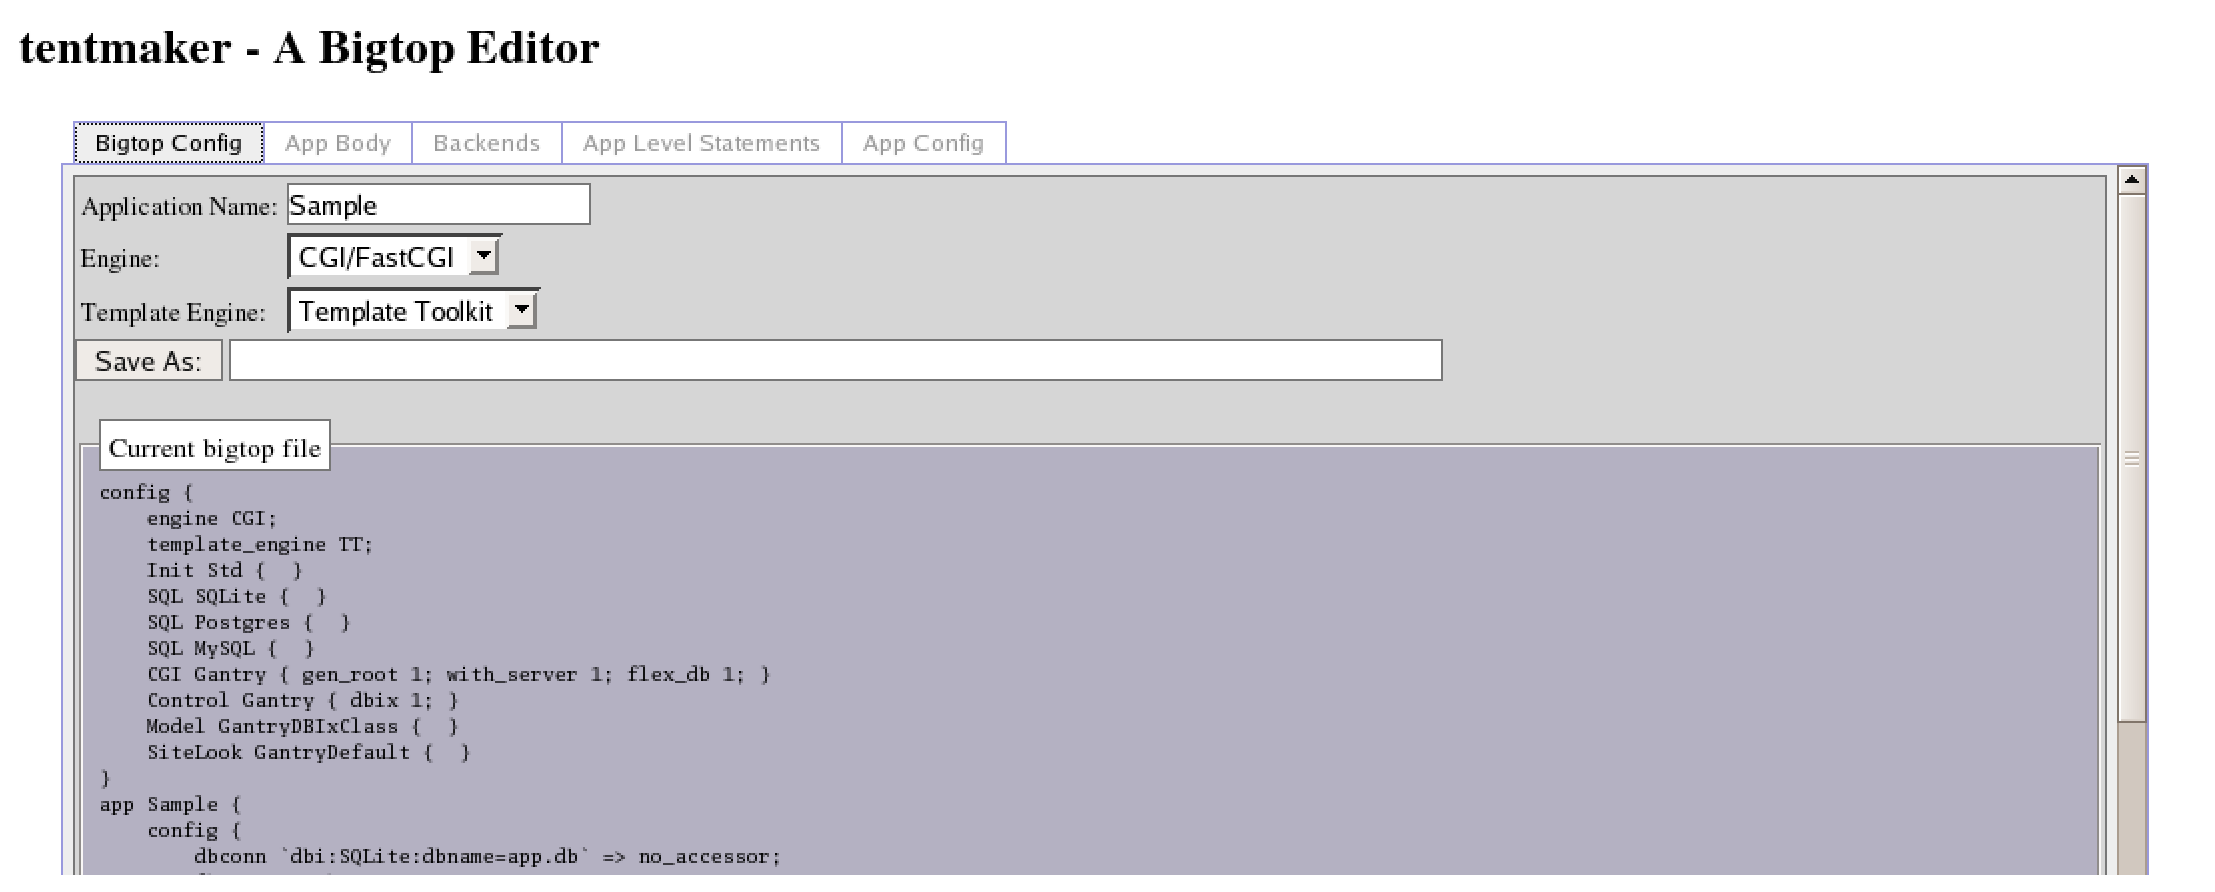
\includegraphics[width=6in]{tentopening}
\caption{The opening appearance of tentmaker.}
\label{fig:tentopening}
\end{figure}

There are five tabs which let you describe your app:

\begin{tabular}{l|l}
Tab Label & Allows you to specify... \\
\hline
Bigtop Config &
    the name of the app and a choice of engines which will serve it \\

App Body &
    the meat of your app, i.e. your tables and controllers \\

Backends &
    the list of all things bigtop should make for you, use check boxes \\
 &  to choose what you want it to do, and input boxes to configure \\
 &  each backend's output \\

App Level Statements &
    author names, their email addresses, project license, etc., all of \\
 &  these have nice defaults \\

App Config &
    a single input table for configuration of your app \\
\end{tabular}

Here we will walk through them in detail.

\subsection*{Bigtop Config}

Let's start at the bottom and move up it.  At the bottom is a dump of the
current bigtop output.  This is mostly for debugging purposes, but look
it over periodically as you have interest.  It is sometimes helpful
when tracking problems.

Immediately above the dump is a `Save As:' button and a file name
box.  When you've made constructive changes, double check the file name and
press the button.  A message will appear, immediately below the button,
telling you how that went.

The top of the tab is more interesting.  Here you can change the name of the
app (which is much easier before initial generation).  You can also choose
a server engine and a template engine.  It is slightly eaiser to start with
the CGI engine and Gantry's stand alone server.  In Chapter \ref{chap:deploy},
we saw how to move to \verb+mod_perl+.

In our shop we like Template Toolkit well enough that we have not added
support to Gantry for any other templating system.  The other alternative
is Default, which turns off templating.  Even with tempating off, you
can still get HTML generation help from Gantry.  The case study in
Chapter \ref{chap:contactus} does this.  You can even use the Template
Toolkit engine manually, when you need to construct special output like
AJAX responses, see Chapter \ref{chap:jobadsapp} for an example.

That is really all there is to say about the first tab.

\subsection*{App Body}

We already had a quick tour through the app body in some prior chapters.
Here we will walk more slowly.

The app body is made up of one or more blocks and statements.  All statements
are managed on the `App Level Statements' tab.  Each block has a type,
most have names.  In the bigtop source file, config is one of the app body
blocks.  It has its own tab (see the last subsection below).  All of the
other types are managed through this tab.

Here are the blocks you can create:

\begin{tabular}{l|l}
Type & Description \\
\hline
Table      & makes an SQL table and corresponding controller              \\
Controller & makes a perl module                                          \\
Literal    & puts literal text into one or more output files              \\
Join Table & indicates two tables which share a many-to-many relationship \\
Sequence   & (rarely used) makes an SQL sequence and corresponding        \\
           & table and controller (useful for Postgres only)              \\
\end{tabular}

Let's look at what you can edit about each of these.

\subsubsection*{Table}

When you open a table for editing, you see something like Figure
\ref{fig:tableedit}.

\begin{figure}
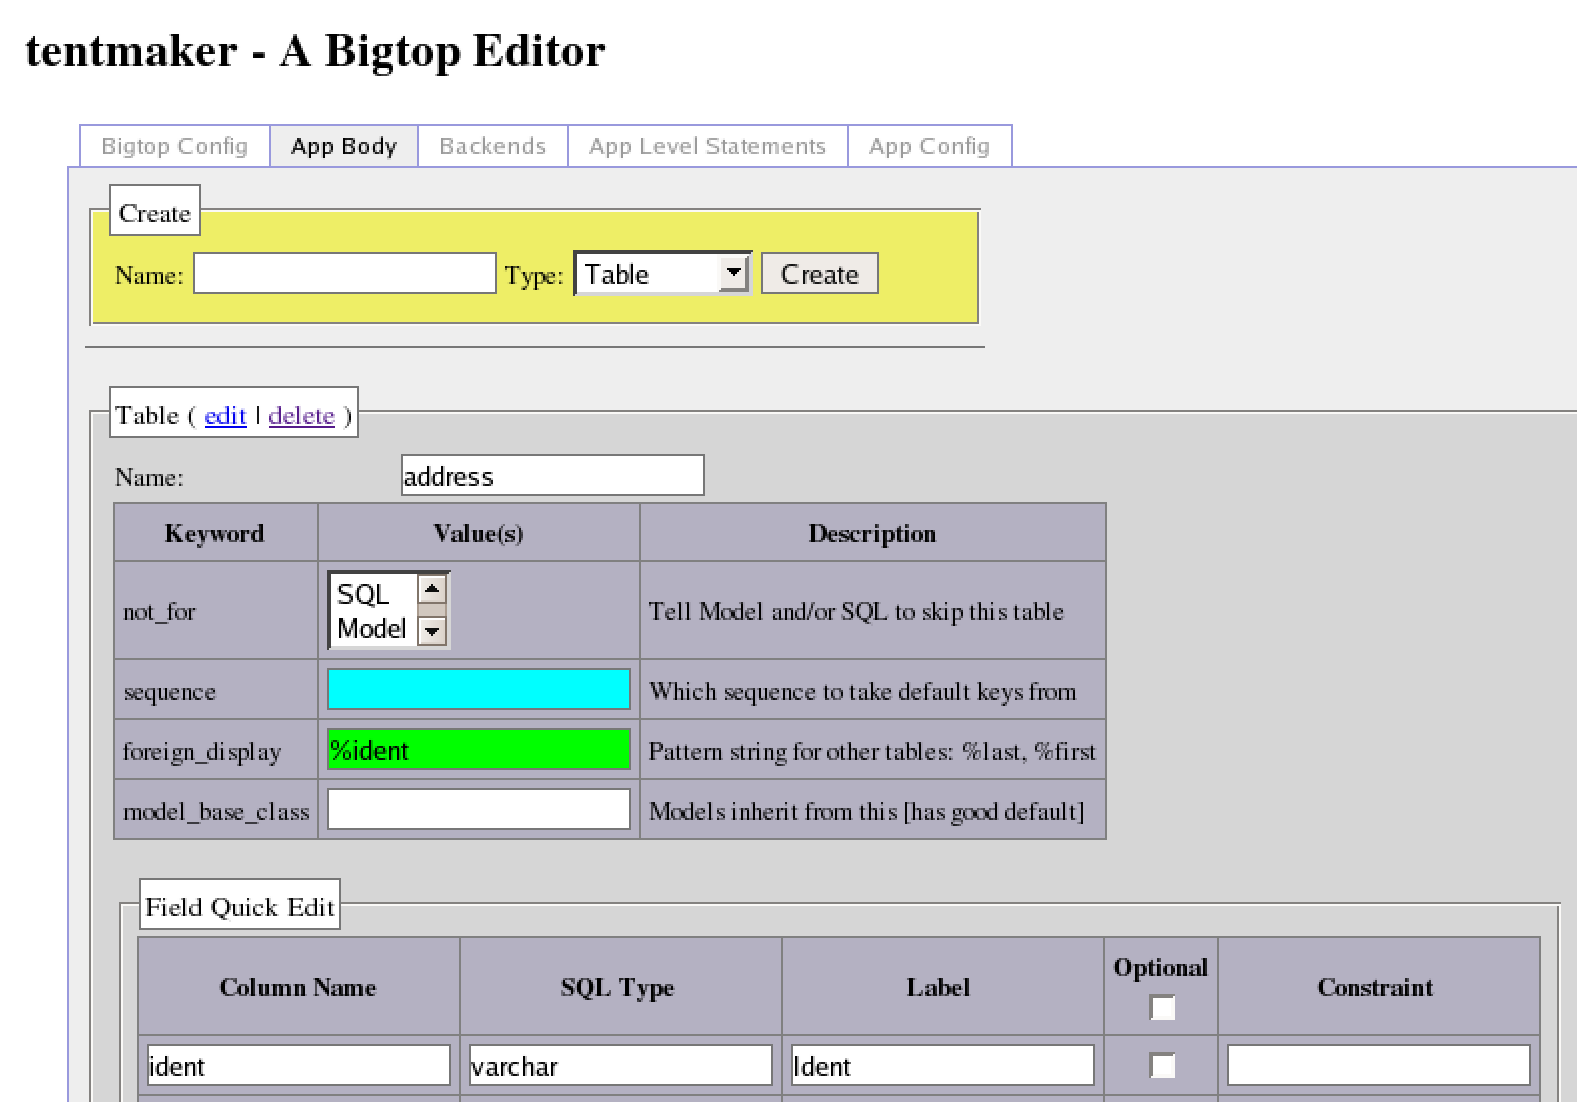
\includegraphics[width=6in]{tableedit}
\caption{Editing a table in tentmaker.}
\label{fig:tableedit}
\end{figure}

From this we see four statements which affect a whole table.  If the table
might offend one of the backends, you can highlight \verb+not_for+ for
that backend.

If you did use a sequence (which we are moving away from) enter its name
in the \verb+sequence+ box.  If you had tentmaker build the sequence for you, it
should have filled that in.

You should probably have a \verb+foreign_display+.  It governs the sort order
of the table when users see all the rows.  It also the summary users will
see when other tables refer to this one via a foreign key.  For example,
if users will select one row from this table as the foreign key value of
another table, this is what they will see in the pull down menu.

The format for \verb+foreign_display+ is simple.  If an ident follows a
percent sign immediately (without whitespace in the middle), it must
be a column name which will be interpolated in at that point.  Everything
else, including trailing percents, is literal.  A common example is
\verb+%last_name, %first_name+, but you can do whatever you like.  Keep in
mind that brevity will probably be appreciated by your users.

Most models should inherit from the default base class, which depends on
the Model backend you choose on the `Backends' tab.  If all of your models
need to inherit from a different base, change it once on the `Backends' tab.
If just this table needs a different base, enter the fully qualified
parent module name here.

Though tables have statements, their main purpose in life is to house
fields.  Fields become columns in the database table and (usually) entry
widgets on the screen.

When you open a field for editing, you see something like Figure
\ref{fig:fieldedit}.

\begin{figure}
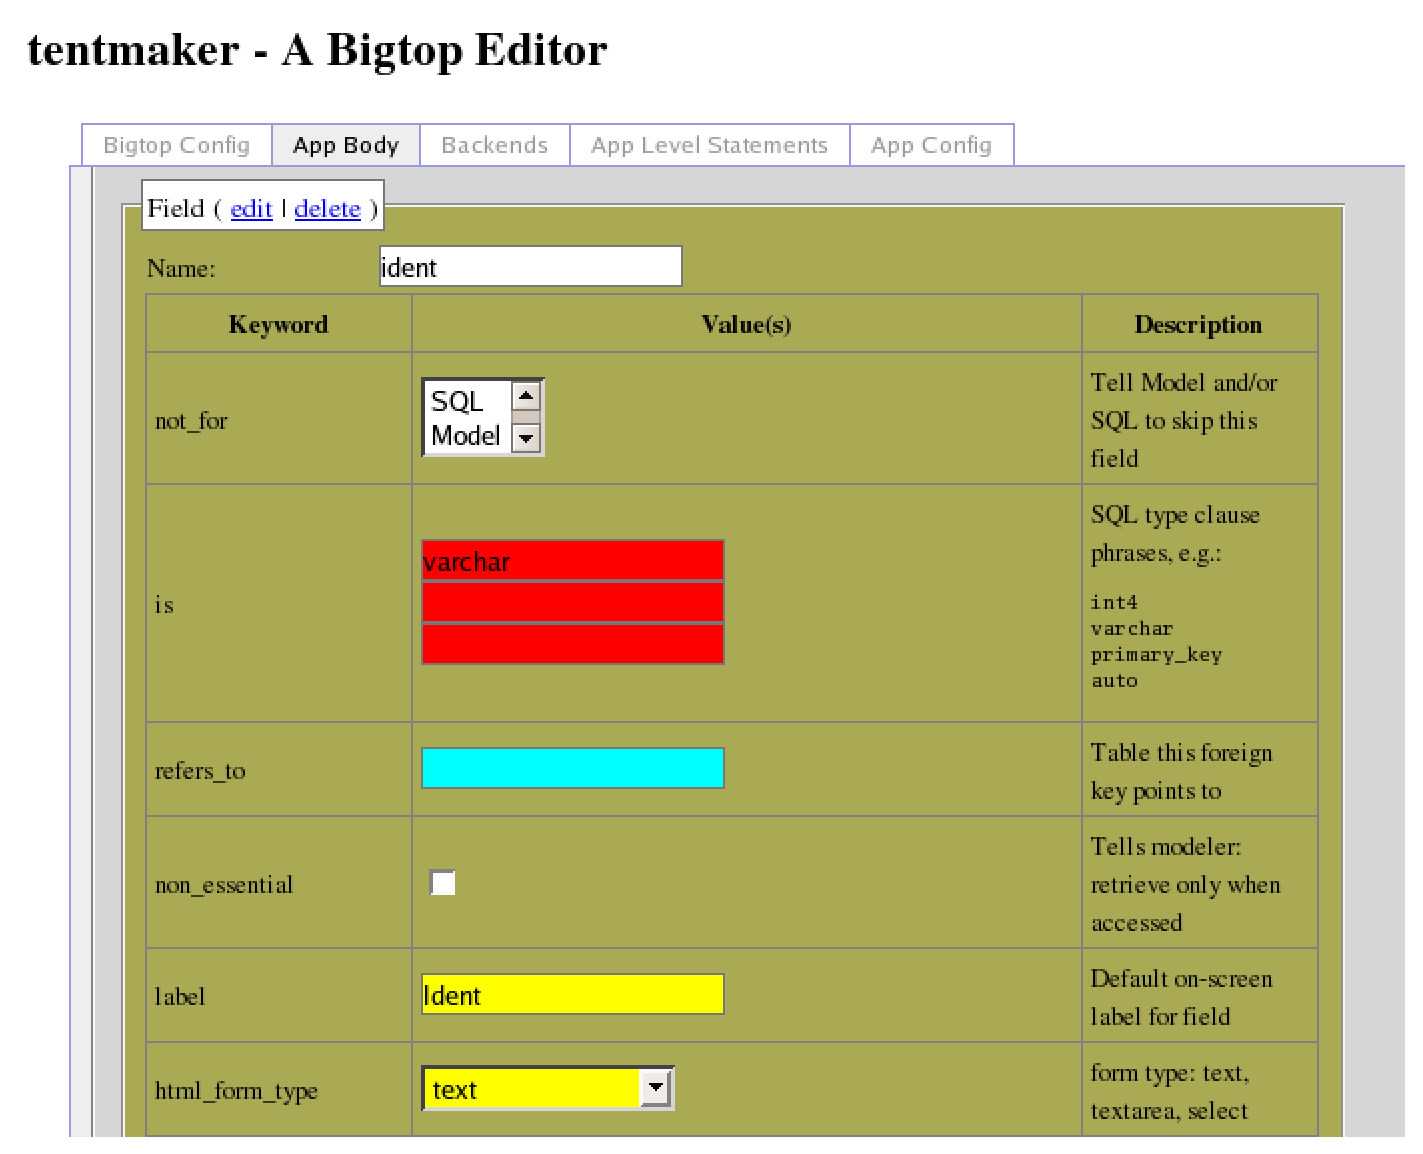
\includegraphics[width=6in]{fieldedit}
\caption{Editing a field in tentmaker (same as Figure \ref{fig:fieldedit1}).}
\label{fig:fieldedit}
\end{figure}

There are many statements that affect fields.  The \verb+not_for+ statement
works for fields just as it does for tables.  This is useful if you have
a column called id which is not the primary key, a situation that confuses
some ORMs.

The \verb+is+ statement accepts SQL phrases for the column defintion.
The most common value is \verb+varchar+, which the backends will translate
to a good string type, if your database doesn't understand it.

You can put as many items in the \verb+is+ statement as you like, one per
box.  There are two highly special items: \verb+primary_key+ and \verb+auto+.
Use \verb+primary_key+ to specify your primary key.  Currently Bigtop and
Gantry don't have much support for multi-column primary keys.  So we
usally stick with the id generated on table creation.

Use \verb+auto+ to indicate that the primary key should be incremented
by the database.  Exactly how that happens is up to the SQL backend
for your database.

The \verb+refers_to+ statement indicates that this column is a foriegn
key pointing to another table.  The other table's name is the value.

Some ORMs use lazy column fetching.  If yours does and the current column
should be fetched lazily (only when an accessor for it is called), check
the \verb+non_essential+ box.

The \verb+label+ is what the user sees whenever the field is on screen.

All of these directly become attributes of the html form elements:
\verb+html_form_type+, \verb+html_form_cols+, \verb+html_form_rows+,
\verb+html_form_display_size+.  The last one becomes the size attribute
of a text input area, since Template Toolkit has a virtual method called
size.

By default, all fields on a form are required.  If you want a field
to be optional, check \verb+html_form_optional+.

The \verb+html_form_constraint+ is used directly by Data::FormValidator,
see its docs for details of what you can put in it.  The short answer
is a regex or a method which returns one.

Any \verb+html_form_default_value+ will be used by the form template
when there is nothing better avaiable.  It must be a literal string or number.

If you want to use a popup date calendar, for a field of type date,
enter a \verb+date_select_text+.

The only statement left is \verb+html_form_options+.  Use this to
enter the options for fields whose \verb+html_form_type+ is select,
unless the field is a foreign key.  Foreign key fields have good
generated selections.

The `Label' of an \verb+html_form_options+ entry is what the user
sees.  The `Database Value' is what goes into the database.  As you
enter options, more boxes appear underneath.  Options appear in the
order the appear in tentmaker.  If you make an error in ordering,
it is usually easier to fix it in a text editor.

\subsubsection*{Controller}

Each controller represents a pair of code modules: a stub module and a GEN
module.  Once written, stubs are never overwritten.  The only ways to get
bigtop to regenerate a stub module are to rename or delete it.

When you edit a controller, you'll something like Figure
\ref{fig:controledit}.

\begin{figure}
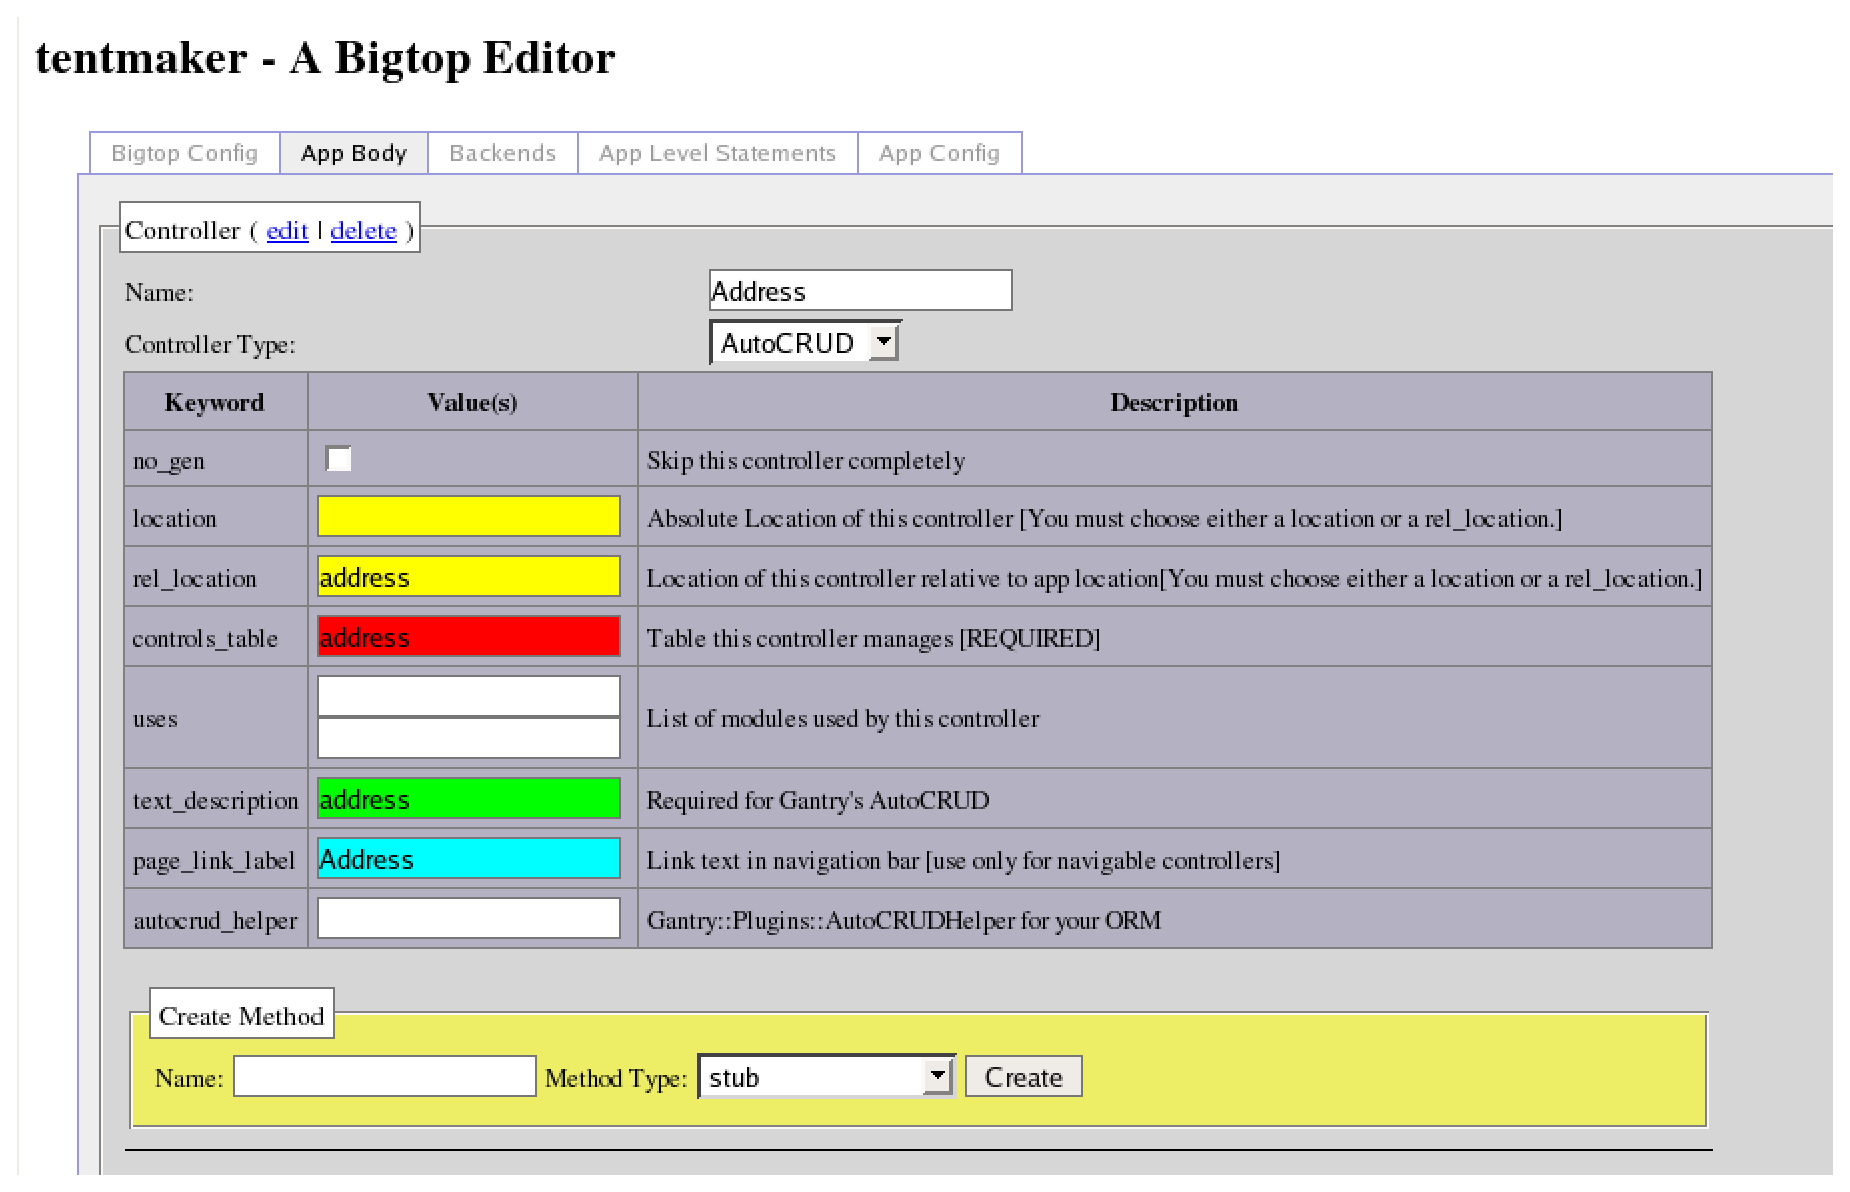
\includegraphics[width=6in]{controledit}
\caption{Editing a controller in tentmaker.}
\label{fig:controledit}
\end{figure}

If you want to skip just one controller, check the \verb+no_gen+ for it.

You must supply either a \verb+location+ or \verb+rel_location+.
\verb+location+ is absolute, \verb+rel_location+ is relative to the
base location for the app.

Most controllers control a single table, enter its name in the
\verb+controls_table+ (if it isn't already there).

If your controller needs external modules, put them in \verb+uses+ boxes.
But, keep in mind that these are most useful in the stubs.  So, using
these won't work after the controller is generated.

The \verb+text_description+ fills in the blank in several sentences for
AutoCRUD.

If you want this controller to appear in site navigation links, give
it a \verb+page_link_label+.  The user will click this label to advance
to this controller's page.

If you have your own ORM scheme, but it doesn't have a backend, specify
an \verb+autocrud_helper+.  It must be a module which responds to the
expected API.  See Chapter \ref{chap:autocrud} for advice.

In addition to the statements in a controller block, there are methods.
When you open a method for editing you see something like Figure
\ref{fig:methodedit}.

\begin{figure}
\includegraphics[width=6in]{methodedit}
\caption{Editing a method in tentmaker.}
\label{fig:methodedit}
\end{figure}

Notice that there is a applies to column in the table.  It tells you which
types of methods can use the statement.

There are three types of methods: stubs, main listings, and forms.  A
stub is just that.  A typical one looks like this:

\begin{verbatim}
#-----------------------------------------------------------------
# $self->stub_name(  )
#-----------------------------------------------------------------
sub stub_name {
    my ( $self ) = @_;
}
\end{verbatim}

You can check \verb+no_gen+ for any method type, causing the backend
to skip it.  You can also supply \verb+extra_args+ for any method these
are added to the end of the argument list at the top of the method
(and in the docs).  Put one argument in each box, remember to include
the sigil.  Further, realize that if the argument is an array, it must
go at the end.

Stub methods are not that much use.  Keep in mind that they only go in
stub modules, so they won't be added once the controller is initially
generated.  The other types are more useful.

The main listing output typically shows all the rows from a simple table
as shown in Figure \ref{fig:main_listingout}.

\begin{figure}
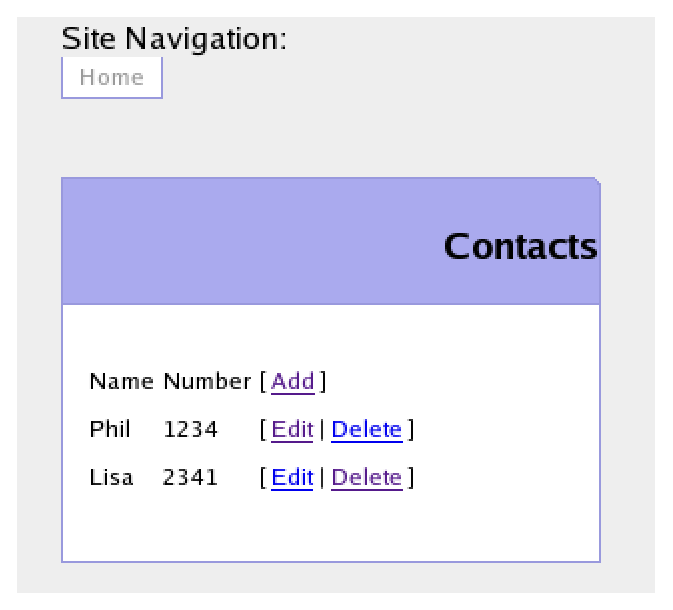
\includegraphics[width=6in]{main_listingout}
\caption{Editing a method in tentmaker.}
\label{fig:main_listingout}
\end{figure}

The \verb+cols+ list names each column of the main listing table.  By
default, these columns are labeled with their field's label.  If you want
to change the label just for the main listing, enter your alternate
labels in the \verb+col_labels+ boxes.  Of course, these must be in the
same order as the \verb+cols+.  Less obviously, skipped boxes are ignored,
not counted.  If you don't supply the same number of labels as their
are columns, the extras will revert to default naming.

At the far right of the main listing output in Figure
\ref{fig:main_listingout}, you see a link labeled `Add.'  That is a
\verb+header_option+.  You can have as many of these as you like.
Normally, they will be handled by a method in the same controller as
the main listing.  The name of the method will be the same as the
label, but in lower case.  If you want a different method to handle
the action, put its location in the `Location,' column.  Even if
some of the `Labels' have alternate `Locations,' you don't have to
specify locations unless the default won't work.

The \verb+row_options+ are similar to \verb+header_options+, but they
apply to each row in the listing.  The most common of these are `Edit'
and `Delete.'  The rules for their locations are the same as for `Add.'
If you construct your own locations, you will want to remember to include
\verb+$id+ at the end of the URL or a query string with that id in it.
Otherwise, the row will be unknown at edit time.

The \verb+title+ is the browser window title.  The \verb+html_template+
defaults to \verb+results.tt+, change it if you like.

All of the remaing statements apply to form methods.  Note that form methods
come in two kinds.  One is for use with AutoCRUD, the other for CRUD.
Their statements are exactly the same.  They only differ in how they
capture their arguments.

The key feature of a form is that it displays a set of entry fields for
columns in the underlying database table.  The first step in setting
one up is to pick the fields.  There are two ways to do that.  Either
enter the fields you want, each one in its own \verb+fields+ input box;
or enter the fields you don't want, each one in its own \verb+all_fields_but+
input box.  I usually do that latter.  That makes it less work when
new fields are added to the table, because in the normal case I want to
enable users to update the new field.

Form methods build hashes which are passed to templates.  Some templates --
including the default form.tt supplied by Gantry -- allow additional
hash keys tentmaker doesn't know about.  The \verb+extra_keys+ take care
of this case. recall that Section \ref{sec:asciiart} has an example involving
a popup calendar.

If your form needs a name (e.g. for CSS use or a popup calendar), enter
it in the \verb+form_name+ input box.

Those are all the statements that apply to methods.  With them, we have
finished talking about controller edits.

\subsubsection*{Literal}

Literals are taken literally.  Each one is understood by at least on backend
or backend family.  They take text directly from your bigtop source file
and dump it into their output.

There are several literal types, this table shows them along with an
explanation of where their output goes.

\begin{tabular}{l|l}
Literal Type & Output Destination \\
\hline
SQL       & docs/schema.*, for all of your SQL backends \\
Location  & the base module location in httpd.conf made by HttpdConf Gantry \\
HttpdConf & between locations in httpd.conf made by HttpdConf Gantry \\
PerlTop   & immediately below the shebang line in <Perl> block of httpd.conf \\
PerlBlock & inside the <Perl> block of httpd.conf \\
Conf      & at the top level of Config::General conf file \\
\end{tabular}

Note that all of the literal types are always legal, but they will be ignored
unless a loaded backend understands them.

When I said that literals are taken literally, I left out one obscure
but pleasant exception.  If your literal does not end with whitespace,
one new line will be added to it in the output.  Otherwise, they are
taken as written.  But, note that how they look in the input box on
the `App Body' tab of tentmaker may be decieving, since some characters
are not visible there (like trailing spaces).  To be sure of what is
in your literal, look at the `Current bigtop file' dump on the `Bigtop
Config' tab.  You could also look at the bigtop file with a text editor.

\subsubsection*{Join Table}

A join table is needed whenever two tables share a many-to-many
relationship.  This table will alwyas have three columns: its own id
and the foreign key ids of the many-to-many tables.  Editing a join
table looks like Figure \ref{fig:joiner}.

\begin{figure}
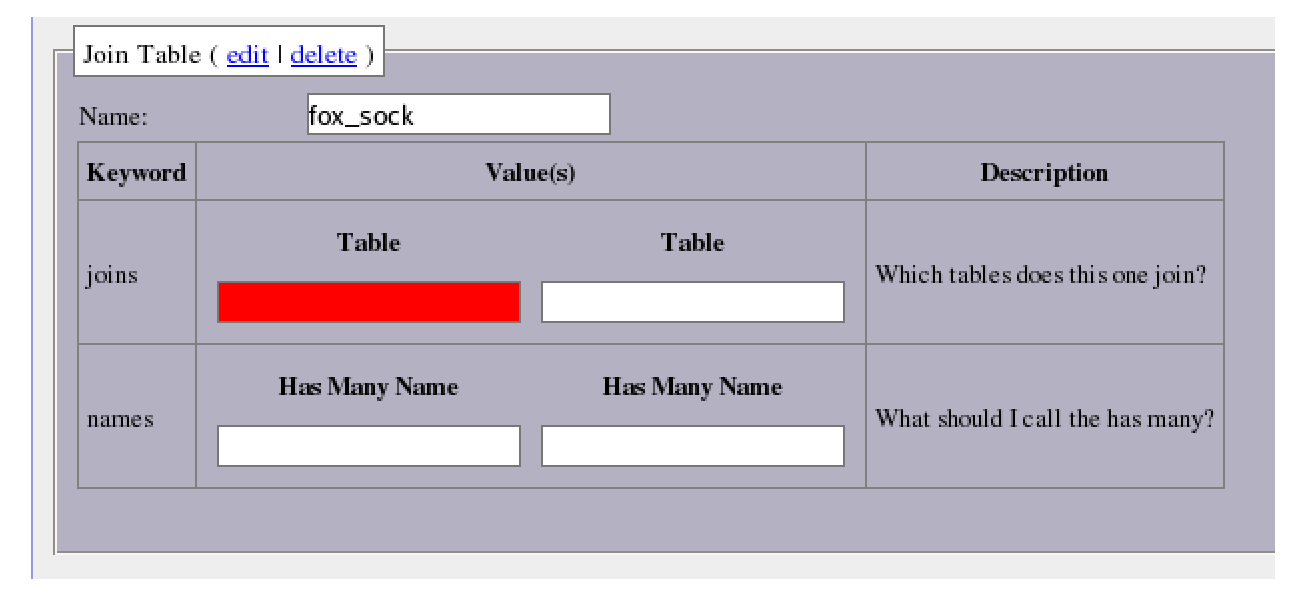
\includegraphics[width=6in]{joiner}
\caption{Editing a join table in tentmaker.}
\label{fig:joiner}
\end{figure}

When using a join table, you must specify the names of the tables it
\verb+joins+ (even if a bug in the CSS doesn't make both boxes red).

For the models to have a many-to-many relationship, you need to use
the Model GantryDBIxClass backend.  It is the only one that understands
them.

Each side of a many-to-many relationship needs a name.  Normally, the
name is the table name with an extra `s' added at the end.  But,
you can control the \verb+names+.  If you pick one, you must pick the
other, even if your choice would be the default.  In Figure \ref{fig:joiner},
the \verb+names+ should probably be `foxes' and `socks.'

A join table is made for you when you use \verb+<->+ in ASCII art for
bigtop or tentmaker.  See Section \ref{sec:asciiart}, or the first section
of this chapter, for how to do that.

\subsubsection*{Sequence}

If you like to use Postgres sequences to auto-increment your primary key,
feel free to create a sequence for each table.  Do this at the outset,
because sequences must be defined before the tables which use them and
because creating a sequence in tentmaker makes a corresponding table
and controller.  Name the sequence with a trailing \verb+_seq+.  Then
the names of the table and controller will make more sense.

Using sequences is not a problem, even if your database does not understand
them.  The backends whose databases don't support them correctly adjust to
a sequence if it is present (mostly by ignoring it).

\subsection*{Backends}

Bigtop can make lots of different things.  The Backends tab controls what
it makes for you.  The basic idea on this tab is simple.  Check the box
for each backend you want working for you.  Once the box is checked, fill
in any values you need for that backend.  See Chapter \ref{chap:backends}
for a list of all available backends and what their configurable values.
When you click the `Backends' tab, you see something like Figure
\ref{fig:backends}.

\begin{figure}
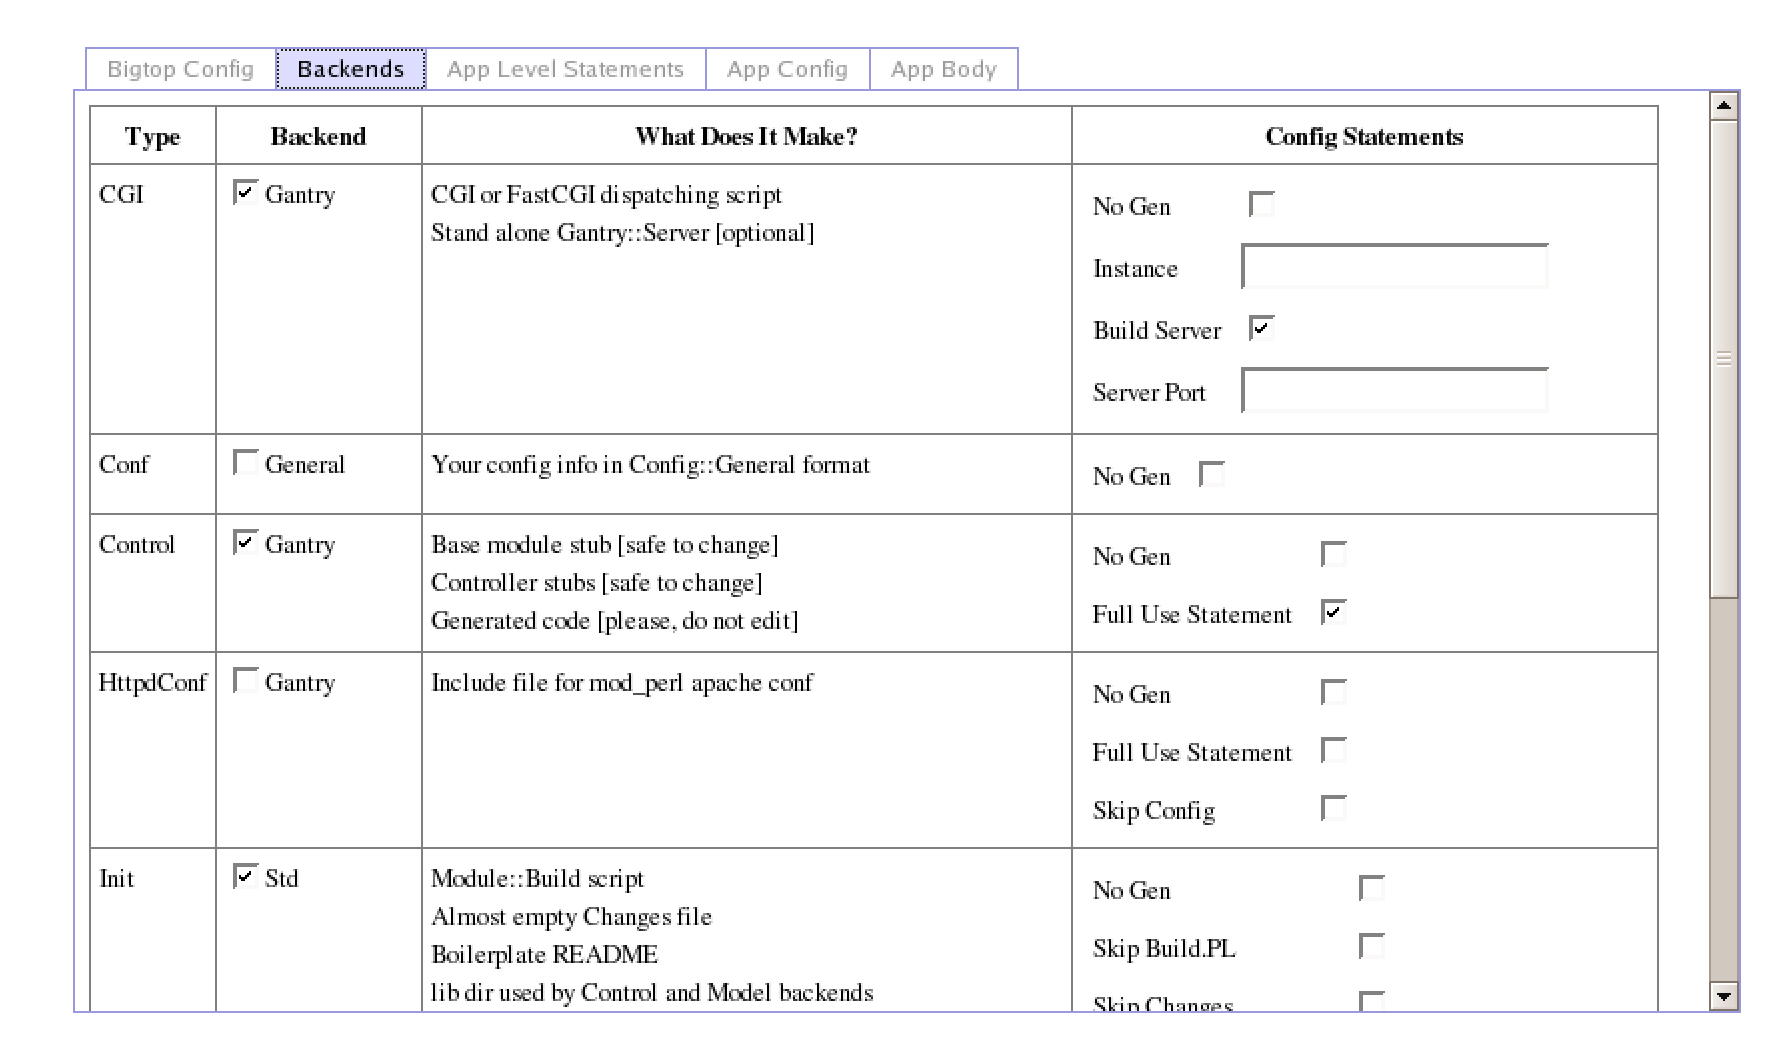
\includegraphics[width=6in]{backends}
\caption{The top of the backends tabbed pane, showing typically available
backends.}
\label{fig:backends}
\end{figure}

I've refrained from including addtional screen shots featuring the othter
backends.  The modules which support tentmaker know how to find all the
backends on your system, so any new ones will show up when you run tentmaker
(see Part IV for how to make your own backends).

Since Chapter \ref{chap:backends} covers them, we'll move along now.

\subsection*{App Level Statements}

App level statements describe the application and its base Perl module.
You must update all of these statements before generation, except `Base
Location.'  Once the base module for the app -- or any other stub module -- is
generated, it is never regenerated.  Bigtop will cowardly refuse to
regenerate stubs.  There is no way to force it to rewrite a stub file short
of deleting or renaming it.

When you edit a default bigtop file, all the app level statements are
blank, so the `App Level Statements' table looks like Figure
\ref{fig:appstat}.

\begin{figure}
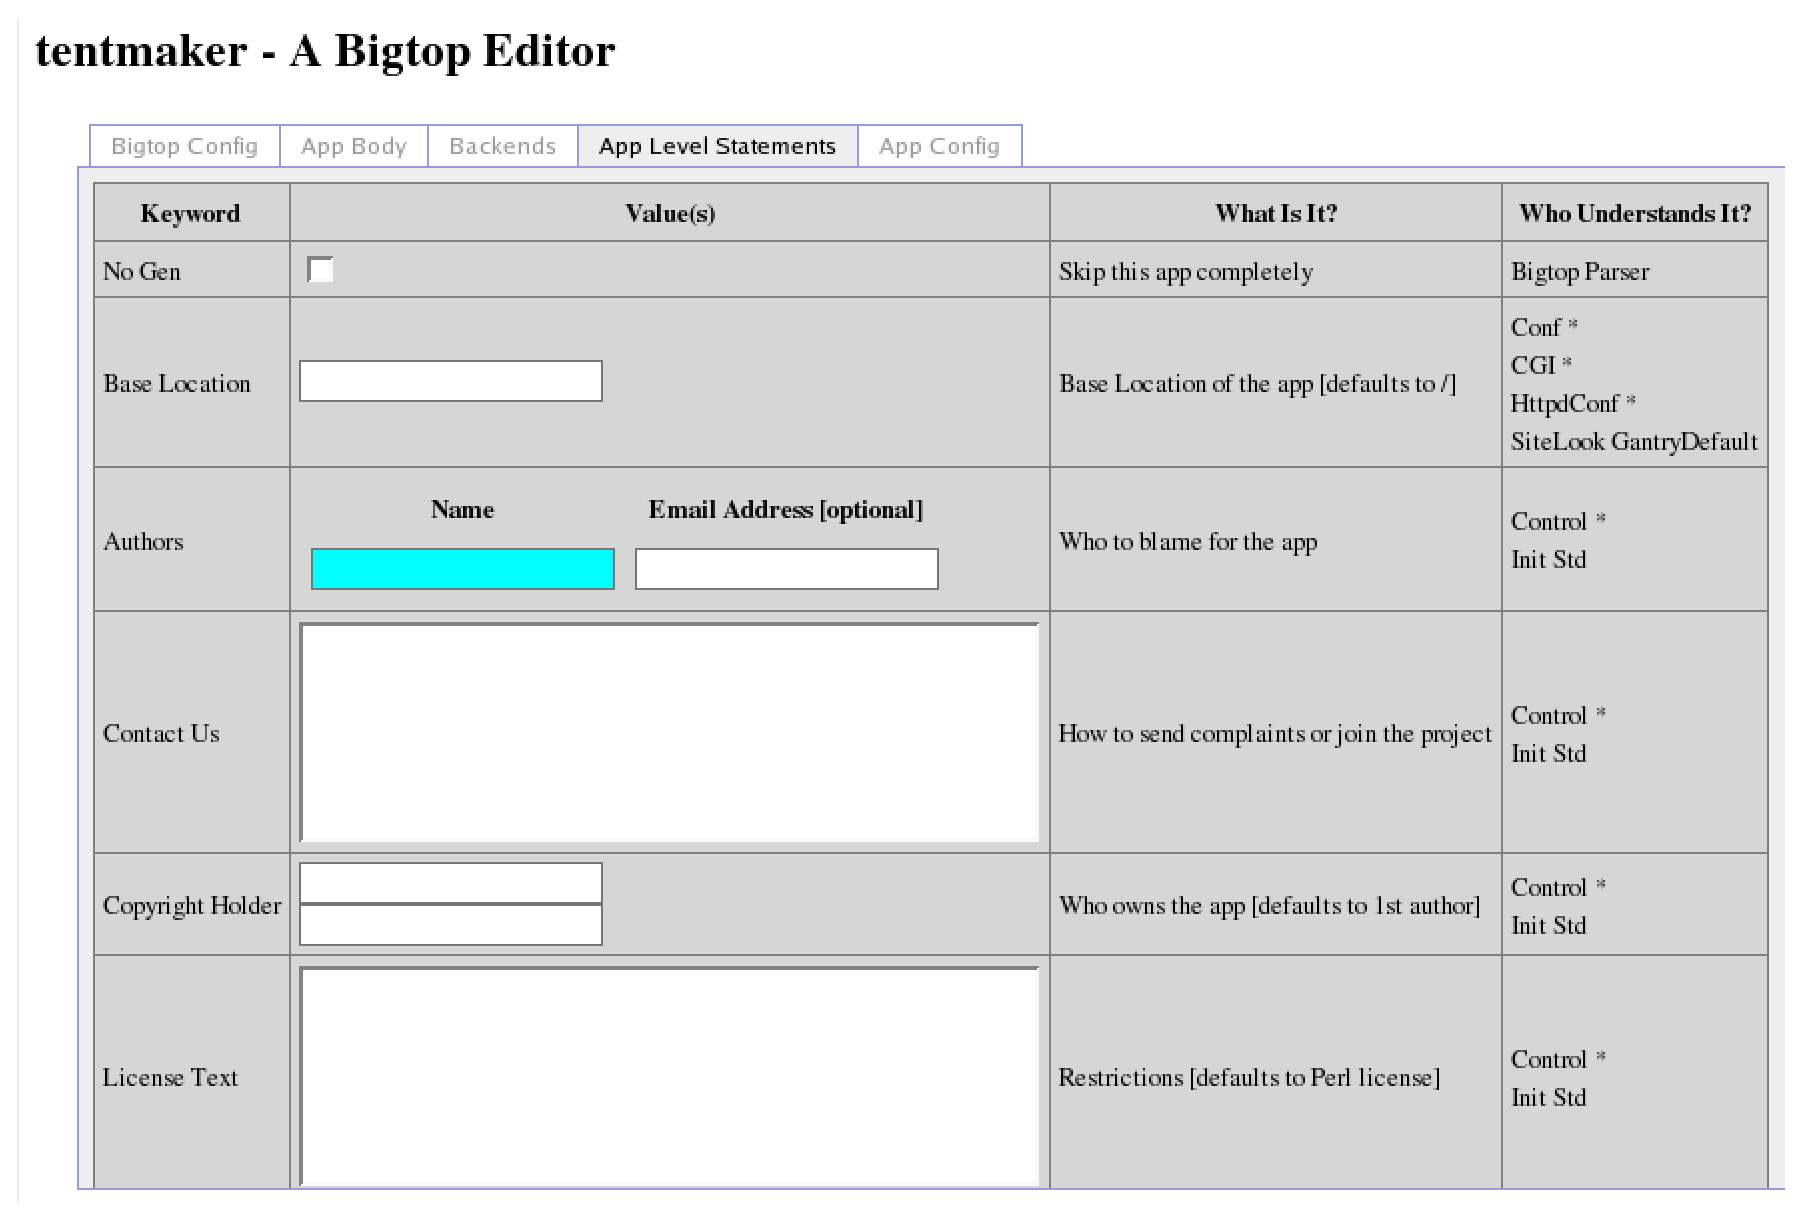
\includegraphics[width=6in]{appstat}
\caption{Editing app level statements in tentmaker.}
\label{fig:appstat}
\end{figure}

All of the things on this tab are optional and have fine defaults.

Truly paranoid people might want to check the `No Gen' box.  Doing
so make the bigtop script skip all generation.

The `Base Location' is the beginning of the URL for all pages in the app.
It is safe to leave it blank.  Then all pages will be at the document
root of the server.  You cannot use a non-trivial `Base Location' with
a stand alone server (like app.server), because it doesn't have a document
root notion.  When you do set a `Base Location,' you need to add an
\verb+app_rootp+ config variable with the same value on the `App Config'
pane (see the next subsection).

If you never enter \verb+authors+, the author name and email will be generated
just like h2xs generates them.  If you do enter `Authors,' you may choose
to supply email addresses.  This is why the name input boxes are colored but
the email input boxes are white.

To add a blurb about joining or contacting your project developers to
various generated docs, enter something for `Contact Us.'

If the first author is not the copyright owner, enter the proper
`Copyright Holder.'

By default, the license text is the same as what h2xs generated for
the Perl 5.8.6 distribution.  If you want something different, enter it
in `License Text.'

Out of view in Figure \ref{fig:appstat} is the `Modules Used' list.  These
will be included in \verb+use+ statements at the top of the base module.
But, keep in mind that the base module will only be written once, so
changes here won't affect one already on your disk.

\subsection*{App Config}

Finally, we come to that last tab.

Most apps have some configuration parameters which should be kept out of
the code, enabling administrators to update them on production machines without
disturbing our beautiful modules.  The `App Config' tab lets you
specify these.  If you started tentmaker without command line data,
there will be three config params already defined, as shown in Figure
\ref{fig:appconfig}.

\begin{figure}
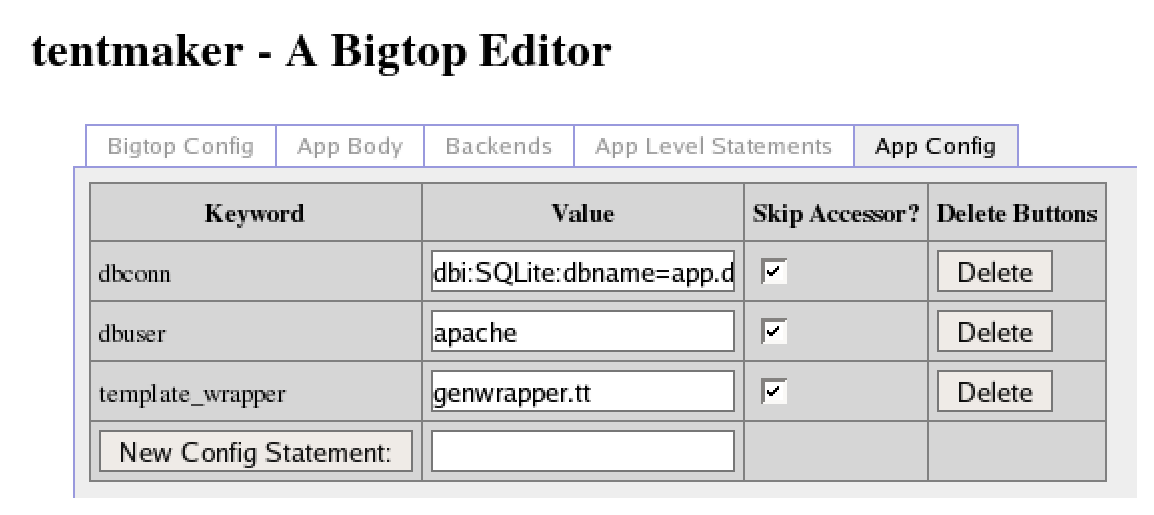
\includegraphics[width=6in]{appconfig}
\caption{Application configuration table.}
\label{fig:appconfig}
\end{figure}

Here you see the DBI connection string.  By default this will use SQLite
as the DBD and call the database app.db.  In earlier examples, we saw
that the stand alone app.server allows users to change this information
at the command line.  In fact, app.server pays no attention to the database
config parameters.  In CGI/FastCGI and \verb+mod_perl+, the information
from the dbconn, dbuser, and (optional) dbpass variables here completely
governs.

By default \verb+template_wrapper+ is set to \verb+genwrapper.tt+.  You
can change that at will to your own wrapper.  The SiteLook GantryDefault
backend makes \verb+genwrapper.tt+.  If you've rolled your own, you don't
need that backend, but you do need to set the name of your wrapper here.

If there are any other config parameters your app needs, feel free to
add them.

Now that we know what tentmaker can already do, you are ready to think big.
But, if you prefer typing to clicking, read the next chapter.  It covers
the syntax of the Bigtop language.  Once you know that, you can type Bigtop
files directly.  More likely, you'll use the information to edit Bigtop
files made by tentmaker.

The subsequent chapters explain how to customize Bigtop to build whatever
you need for your apps.  As you build things, they become available
through tentmaker as soon as you install them on your system (or sooner
if you add a use lib to your tentmaker).
       % comprehensive guide to tentmaker
\chapter{Bigtop Syntax}
\label{chap:bigsyntax}

This chapter follows up on the previous chapter by providing Bigtop source
file syntax documentation.  While tentmaker is frequently convenient, and
it sure types more accurately than I do, it can be tedious for some edits.
In those cases, a good text editor can be a life extender.

The definitive word on what statements can appear in a Bigtop file is
maintained by Bigtop::Keywords.  It is used by all the current backends
and thus provides a standard place to make the definitions.  I refered
to it heavily while writing this.  If you are writing a backend, it is
vital for everyone's sanity that you place your keywords there instead
of in some ad hoc place.

\section{Basic Structure}

Bigtop files have a basic structure.  At the top level, there are two
blocks:

\begin{verbatim}
config {
}
app Name {
}
\end{verbatim}

Inside the blocks there are statements and blocks.  Statements usually have
a single keyword followed by a value and a semi-colon (literal statements
are an exception to that rule, see below).  Block structures vary depending
where they appear.  It is easier to understand this with an example.
Here is the smallest one that bigtop or tentmaker will make with the new
flag:

\begin{verbatim}
config {
    engine CGI;
    template_engine TT;
    Init Std {  }
    SQL SQLite {  }
    SQL Postgres {  }
    SQL MySQL {  }
    CGI Gantry { gen_root 1; with_server 1; flex_db 1; }
    Control Gantry { dbix 1; }
    Model GantryDBIxClass {  }
    SiteLook GantryDefault {  }
}
app Test {
    config {
        dbconn `dbi:SQLite:dbname=app.db` => no_accessor;
        template_wrapper `genwrapper.tt` => no_accessor;
    }
    table tbl1 {
        field id {
            is int4, primary_key, auto;
        }
        field ident {
            is varchar;
            label Ident;
            html_form_type text;
        }
        field description {
            is varchar;
            label Description;
            html_form_type text;
        }
        field created {
            is datetime;
        }
        field modified {
            is datetime;
        }
        foreign_display `%ident`;
    }
    controller Tbl1 is AutoCRUD {
        controls_table tbl1;
        rel_location tbl1;
        text_description tbl1;
        page_link_label Tbl1;
        method do_main is main_listing {
            cols ident, description;
            header_options Add;
            row_options Edit, Delete;
            title Tbl1;
        }
        method form is AutoCRUD_form {
            all_fields_but id, created, modified;
            extra_keys
                legend => `$self->path_info =~ /edit/i ? 'Edit' : 'Add'`;
        }
    }
}
\end{verbatim}

Here we see the basic structure of a bigtop file, the remaining sections in
this chapter explain all of the legal syntax which can go in that structure.

\section{The config Block}

In normal use, a config section can have only two statements
(there are deprecated statements not covered here):

\begin{tabular}{l|l}
Keyword & Example Values \\
\hline
\verb+engine+ & CGI, MP13, or MP20 (the later two are for \verb+mod_perl+) \\
\verb+template_engine+ & TT or Default \\
\end{tabular}

The \verb+engine+ is the framework engine you will use.  Gantry supports
CGI -- which also works for Fast/CGI -- and \verb+mod_perl+ 1.3 and 2.0.
Use MP13 or MP20 for \verb+mod_perl+.

The \verb+template_engine+ is the framework template engine you will use.
Gantry support TT -- for Template Toolkit -- or Default.  The Default
template engine does absolutely nothing, thus allowing you complete control
over what is returned to the browser.

Blocks in the Bigtop config block have two names and a set of statements
in braces.  The set of statements could be empty.  Use statements to tweak
what the backend will generate.  This chapter will not cover the statements,
since they are already fully discussed in Chapter \ref{chap:backends}.

The names of a backend block give its type (or family) and its name.
Again, all of those are discussed in Chapter \ref{chap:backends}.
If you work in the Bigtop, just use the type and backend names
as discussed there.  For example. if you want MySQL output, include
this block:

\begin{verbatim}
    SQL MySQL {}
\end{verbatim}

SQL is the backend type, there are others of the same type: Postgres and
SQLite.  MySQL is the name of the backend.  Consult tentmaker for a list
of all backends installed on your system.  The remaining chapters in this
part of the book explain how to write your own backend.

\section{The app Block }

The app block of a bigtop file is far more interesting than the top level
config block.  It contains the configuration information for the app,
together with a description of its tables and controllers.  This section
has subsections for each block type in the app block.  But let's start
with a subsection on app level statements.

\subsection*{App Statements}

As with the top level config block, the app block can have statements.
We will now cover the same ground as the `App Level Statements' subsection
of Chapter \ref{chap:tentref}, but with a focus on Bigtop syntax rather
than where to click in tentmaker.

Note that there are different types of statement values.  In general,
statements may accept comma separated lists of values.  Each element in
that list may be a single item or a pair.  If it is a single item,
it must either be a number, a valid Perl ident, or be enclosed in backquotes.
Yes, I said backquotes.  These make it easier to embed Perl's other quotes.
I figure you shouldn't need Perl's backquotes in a web app.

Pairs are separated with fat commas: \verb+=>+.  These are not related
to commas.  In Perl, a fat comma is a comma which forces its left argument
to string context.  In Bigtop a fat comma makes a hash with a single key.

The \verb+authors+ statement provides a good example of value variety:

\begin{verbatim}
    authors `Phil Crow` => `philcrow2000@yahoo.com`, `Joe Doe`, Bill;
\end{verbatim}

There are three items in this list.  The first one is a pair.  The other
two a single values.  OK, so Bill isn't quite so helpful as the first item
in the list, but it is legal.  Note the use of backquotes to hide spaces,
at signs, or anything else Perl wouldn't like in an identifier.

Note that other statements may or may not allows mulitple values and/or
pairs as indicated in the table:

\begin{tabular}{l|l|l}
Keyword & Meaning & Values \\
\hline
\verb+location+         & Base URL absolute from doc root & one string \\
\verb+authors+          & Who works on the app & multiple strings or pairs\\
\verb+contact_us+       & How to join the app & one string \\
\verb+copyright_holder+ & Who owns the app & one string \\
\verb+license_text+     & Exact text & one string \\
\verb+uses+             & Modules used in base module & multiple module names\\
\end{tabular}

Note that most of these will have no effect after initial generation.
All of them except \verb+location+ and \verb+uses+ only put things into
stub code.  Stub code is never overwritten.  It is possible that the
README will be updated with these values on regeneration, but most people
turn off Init generation.

\verb+uses+ will be effective after initial generation, but only because
it puts things into the GEN module.  It will not put use statments into the
stub after it is written.

\subsection*{Literals}

Literals allow you to put literal text directly into generated output.
In order to control which backends use your literal content, literals have a
type.  So they look something like this:

\begin{verbatim}
    literal SQL `INSERT INTO tbl1 ( ident ) VALUES ( 'somename' );`;
\end{verbatim}

The type of this literal is `SQL,' meaning that only SQL backends will
respond to it.  At present all literals have a single type, so all SQL
backends will use all literals of that type.

The value of each literal must be enclosed in backquotes and will be used
as is, with one exception.  If you don't have trailing whitespace, one new
line will be added to the literal.

The `Literal' subsubsection of Chapter \ref{chap:tentref} has a complete
list of the literal types and where their output goes.

\subsection*{Tables}

A table block looks basically like this:

\begin{verbatim}
    table name {
    }
\end{verbatim}

Inside the block you may use table statements or include field blocks
(described below).  Here are the legal statements:

\begin{tabular}{l|l|l}
Keyword & Meaning & Values \\
\hline
\verb+no_gen+  & Boolean for skip this table & Perl truth \\
\verb+not_for+ & Backend types which skip this table & SQL, Model, or both \\
\verb+sequence+         & Name of sequence block for this table & one ident \\
\verb+data+ & Initial SQL data (repeatable) & list of column value pairs \\
\verb+foreign_display+  & How other tables see our rows & one string \\
\verb+model_base_class+ & What model inherits from & one module \\
\end{tabular}

Note that boolean statements evaluate their values for Perl truth.  Usually,
I use \verb+1+ for true and leave the statement out for false.

To list both \verb+not_for+ choices, put them in a list (order doesn't matter):

\begin{verbatim}
        not_for SQL, Model;
\end{verbatim}

Most statements in Bigtop must be unique within their block, but data
statements are an exception.  Repeat these to create as many rows as your
table needs:

\begin{verbatim}
    data ident => INPROG, descr => `Working on it`;
    data ident => BILLED, descr => `Bill has been sent`;
\end{verbatim}

Duplicating other statements leads to unpredictable results, which may
include fatal errors or corrupted output.

\subsubsection*{Fields}

Fields describe columns in SQL tables and entry elements on HTML forms
where users supply that data.  They allow these statements:

\begin{tabular}{l|l|l}
Keyword & Meaning & Values \\
\hline
\verb+no_gen+  & Boolean for skip this field & Perl truth \\
\verb+not_for+ & Backends which skip this field & SQL, Model, or both \\
\verb+is+ & SQL column definition clauses & a list of strings, see below \\
\verb+refers_to+ & Foreign table this field refers to & one table name \\
\verb+label+ & On screen label for field & one string \\
\verb+non_essential+ & Boolean for delayed fetch & Perl truth, see below \\
\verb+date_select_text+ & Link text for popup calendar & one string \\
\end{tabular}

In addition to those statements, there are a set of statements which are
passed through to the form template.  These all have the \verb+html_form_+
prefix, which is stripped before passing the data to the template.  The
names are completely governed by the template, but they should be listed
in Bigtop::Keywords and must be registered by a backend.

Here are all of the form template statements, without their prefix:

\begin{tabular}{l|l|l}
Keyword & Meaning & Values \\
\hline
\verb+type+  & form element type & one of text, textarea, or select \\
\verb+optional+ & Boolean for whether the user can skip it & Perl truth \\
\verb+constraint+ & Data::FormValidator constraint & one string \\
\verb+default_value+ & Default form element value & one string \\
\verb+cols+ & cols attribute of textarea HTML element & one positive int \\
\verb+rows+ & rows attribute of textarea HTML element & one positive int \\
\verb+display_size+ & size attribute of text HTML element & one positive int \\
\verb+options+ & pull down menu choices & list of label => value pairs \\
\end{tabular}

I would have chosen \verb+size+ instead of \verb+display_size+, but
Template Toolkit has a virtual method called \verb+size+.

You may have as many values for the \verb+html_form_options+ statement
as you like.  All of them must be pairs where the key is a string, number,
or ident and the value is also a string, number, or ident.  The key will
be the visible label of the option in the menu.  The value will be used
in the database.  Careful use of these can eliminate the need for certain
coding tables.

\subsection*{Join Tables}

Join tables represent a many-to-many relationship between two tables
defined elsewhere in the bigtop file.  They actually become a third
table with foreign keys to the tables at the ends of the many-to-many
relationship.  The name of the \verb+join_table+ block is the name of the
third table.

Join table blocks can only have two statements.  The \verb+joins+ statement
is required.

\begin{tabular}{l|l|l}
Keyword & Meaning & Values \\
\hline
\verb+joins+ & which tables are being joined & one of pair of table names \\
\verb+names+ & what the relationship should be called & one of pair of names \\
\end{tabular}

If you don't supply a \verb+names+ statement, the many-to-many relationships
are named by taking the end point tables and appending `s' to their names.
You can change that by including a \verb+names+ statement.  Note that if you
want to name one table, you must name both tables.  Here's a complete
example:

\begin{verbatim}
    join_table fox_sock {
        joins fox => sock;
        names foxes => socks;
    }
\end{verbatim}

\subsection*{Controllers}

Controller blocks describe controller modules.  Most of these control
one table through using its model.  They may have statements, just like
other blocks.  They may also have method blocks, contol level literals
and control level config blocks.  The later have their own subsections
below.  Here are the controller level statements:

\begin{tabular}{l|l|l}
Keyword & Meaning & Values \\
\hline
\verb+no_gen+ & boolean for skip this controller & Perl truth \\
\verb+location+ & absolute location to this controller & one path \\
\verb+rel_location+ & location for this controller relative to root controller
                    & \\
                & & one path \\
\verb+controls_table+ & name of controlled table & one table name \\
\verb+uses+ & modules used by this controller & list of installed modules \\
\verb+text_description+ & for AutoCRUD on screen prompting & one string \\
\verb+page_link_label+ & Nav link label for page & one string \\
\end{tabular}

If you don't want the GEN module for the controller to be regenerated,
set \verb+no_gen+ to one (or your favorite true value).  Remember that
the stub is never regenerated, unless it is missing.

You must have either a \verb+location+ or a \verb+rel_location+.  If you
use a \verb+location+, it may be any valid URL; \verb+rel_locations+ will
have the app's root location prepended.

If you don't want the page to appear in site navigation links, don't include
a \verb+page_link_label+.

With the statements out of the way, let's look at the other things which
can go inside a controller block.

\subsubsection*{Methods}

Methods are full blocks, complete with types.  They look like this:

\begin{verbatim}
        method do_something is stub { ... }
\end{verbatim}

The type can be anything your Control backend understands.  Currently that
includes \verb+stub+ (which has only an opening comment, a declaration,
and parameter handling), \verb+main_listing+, \verb+AutoCRUD_form+, and
\verb+CRDU_form+.  The later make forms for use with Gantry's CRUD schemes.

Method statements are all legal no matter what type of method you have,
but they are likely to be ignored if you use them where they don't apply.
Thus, there is an extra column in the following table (as there is in
tentmaker):

\begin{tabular}{l|l|l|l}
Keyword & Applies to & Meaning & Values \\
\hline
\verb+no_gen+ & All & Skip this method & Perl truth \\
\verb+extra_args+ & All & extra params sub should accept
              & list of backquoted variable names (with sigils) \\
\verb+cols+   & \verb+main_listing+ & columns in main listing
              & list of field names \\
\verb+cols_labels+ & \verb+main_listing+ & column labels
              & list of column labels \\
\verb+cols+   & \verb+main_listing+ & columns in main listing
              & list of field names \\
\verb+header_options+ & \verb+main_listing+ & main table heading options (Add)
              & list of options \\
\verb+row_options+ & \verb+main_listing+ & options for each main table row
              & list of options \\
\verb+title+ & \verb+main_listing+ & browser title for main listing page
              & one string \\
\verb+html_template+ & \verb+main_listing+ & what to use instead of results.tt
              & one template name \\
\verb+extra_keys+ & \verb+forms+ & extra keys for returned form hash
              & list of key/value pairs \\
\verb+fields+ & \verb+forms+ & list of fields to include on form
              & list of field names \\
\verb+all_fields_but+ & \verb+forms+ & list of fields to exclude from form
              & list of field names \\
\verb+fields+ & \verb+forms+ & name attribute of HTML form element
              & one ident \\
\end{tabular}

Normally, main listing columns are labeled with their fields' labels.
If you want to override the label, just for the main listing, supply
\verb+col_labels+.  If your list runs out before the \verb+cols+ list,
the extras are again named for their fields.

The \verb+header_options+ values are similar to \verb+authors+ values
at the app level.  They can be single idents, like Add.  But they can
also be pairs, where the value is the URL to hit when the user chooses
the option.  By default the URL is the current controller with
\verb+/option+ appended.  This leads to the \verb+do_option+ method.
So, the default URL is formed by tacking the lower case of the option name
onto the end of the current location.

The \verb+row_options+ are similar to \verb+header_options+, but they
apply at the end of each row in the main listing.  There is one difference:
the default locations have the current row id appended to the URL.
If you supply non-default URLs, be sure to manually add \verb+$id+.

\subsubsection*{Controller Literals}

There are two types of literals which may appear inside controller blocks.
Like app level literals, they have a type name and a string.

\begin{tabular}{l|l}
Type & Destination \\
\hline
Location & inside httpd.conf Location block for the controller \\
GantryLocation & inside GantryLocation block in Gantry::Conf file \\
\end{tabular}

These will be ignored unless you use a backend which understands them.
The HttpdConf Gantry backned understands \verb+Location+, while
the Gantry Conf backend understands \verb+GantryLocation+.

Remember to put the literal value in a backquoted string (bare idents
are not allowed).  Also remember that if your literal value does not
have trailing whitespace, the backend will add one trailing blank line.

\subsubsection*{Controller Configs}

As the app level has a config block, so does each controller, even though
we almost always use the one at the app level and almost never use them
at the controller level.  These blocks allow you to provide config info
that only one controller understands, or to override global config info
with specific values for the benefit of individual controllers.

The syntax for these is exactly like their app level cousins, except that
the block must be placed inside a controller to affect just that controller.
There is no way to have some config information that is available to
a subset of controllers.  It is either at the app level for all or in
a controller block for one.

\subsection*{Sequences}

Sequences are only understood by Postgres.  Though sequences need to be
represented by a block, it must be empty.  Eventually, we may add sequence
statements to control minimum values and the like.  For now you get a
default sequence:

\begin{verbatim}
    sequence name {}
\end{verbatim}

Now that you have seen all the syntax Bigtop has to offer, I wish you
happy editing.  It is frequently useful to pair the knowledge of this
chapter with a good understanding of tentmaker to gain the greatest
efficiencies.  The clicking in tentmaker can be tedious, but it has
some deep magic.  Typing in an editor requires careful attention to
syntax, but makes mass edits easier.  Use the style that makes sense.
     % comprehensive guide to bigtop syntax
\chapter{Parsing Background}
\label{chap:parsing}

This chapter introduces the basics of parsing theory, as implemented by
Parse::RecDescent, so everyone has a chance to write backends for
Bigtop.  The remaining chapters in this part of the book explain
how to apply the parsing knowledge from this chapter so you can write
backends.

Now there is much more to parsing than I can say here.  Whole books are
written that only cover parts of the field.  Here I will focus on the
things you need to know to work with Bigtop as a backend author.

In particular, this chapter sticks to recursive descent parsing, since
that is what Bigtop uses.  Further, we are aiming for the particular
recursive descent parser: Parse::RecDescent.

If you want to study parsing at greater length I recommend the Dragon book,
Compilers: Principles, Techniques, and Tools by Alfred Aho, Ravi Sethi, and
Jeffrey D. Ullman.  This classic has a recent new edition.  The first chapter
is especially important to understanding how to parse.

\section{Parsing a Small Language}

Instead of taking an abstract approach to parsing, I'll focus on Bigtop.
To start, imagine that Bigtop were simpler, so simple that it had only one
block type: field.  Further, let's limit ourselves to just two statements:
\verb+refers_to+ and \verb+html_form_type+.  Once we can parse that, it's
not really so big a leap to understand how Bigtop::Parser uses
bigtop.grammar to parse the full Bigtop language.

To start, our language will only allow something like:

\begin{verbatim}
field name {
    refers_to foreign_table;
    html_form_type select;
}
\end{verbatim}

That is, each legal block will begin with the literal `field' followed
by a name and a block.  Inside the block will be one or more statements
made up of a keyword followed by a value and ending with a semi-colon.
For now only two keywords will be allowed.  Further, let's limit the
legal values for the \verb+html_form_type+ to \verb+select+, \verb+text+,
or \verb+textarea+.  Even though Bigtop does not make that limitation,
it will show you a bit more about parsing.

Let's start at the bottom level and work up.  Fundamentally, we need
to know what a valid name looks like.  For now, we'll use our valid name
definition to match both keywords and \verb+refers_to+ values.  In Bigtop
valid names -- also called identifiers -- begin with a letter and are
followed by one or more letters, numbers, or underscores.  (Some of them can
also include double colons to align them with Perl class names, but that's
getting ahead of our simple example.)

Here's the bigtop.grammar rule which defines valid identifiers:

\begin{verbatim}
IDENT : /^\w[\w\d_]*/
\end{verbatim}

This is as simple as a Parse::RecDescent rule can be.  On the left side
of the colon is the internal name of what we are defining.  Since it
is at the lowest possible level, I named it in all caps.  These are called
tokens in parsing theory.  Everything in the language is first matched
as a token.  The colon separates an item being defined from the legal
values it describes.  Here, the right hand side is just a regex.  (Astute
readers will note that \verb+\w+ allows numbers, which are not actually
valid identifiers.  Bigtop users are left with broken output if they
use leading numbers, since the grammar does not complain.  But, this long
time bug doesn't seem to cause users much grief.)

Grammar rules are also called productions.  IDENT has a single production.
Later, we will see grammar elements which can take several forms.  Each
legal form is described by a separate production (or alternative).

To limit \verb+html_form_types+, we need a rule like this:

\begin{verbatim}
HF_TYPE : 'select' | 'text' | 'textarea'
\end{verbatim}

The token for these legal types is \verb+HF_TYPE+ (the name is arbitrary).
The value can be \verb+select+ or \verb+text+ or \verb+textarea+.  So,
the pipe symbol \verb+|+ is used in grammar rules just as it is in regexes:
to represent alternatives.  Just as in regexes, alternatives in recursive
descent parsing are checked one at a time in the order listed.  As
soon as one matches the others are not tried.  This may seem odd to those
familiar with yacc style parsing, where the length of the matched string
matters.  Here the length is not considered, since only one production
is tried at a time.

Parse::RecDescent literals are surrounded by single quotes like the various
form types are in the \verb+HF_TYPE+ definition.

Now that we have defined our tokens, we can move up a step and define
statements:

\begin{verbatim}
field_statement : 'refers_to' IDENT ';'
                | 'html_form_type' HF_TYPE ';'
\end{verbatim}

This says that each field statement must begin with either \verb+refers_to+
or \verb+html_form_type+ and refers to statements should be tried first.
After \verb+refers_to+, the first production requires any valid \verb+IDENT+
followed by a literal semi-colon.  The \verb+IDENT+ is the name of the
foreign table this field points to.

If the refers to production cannot match for any reason, the next
alternative production is tried.  In this case that is the
\verb+html_form_type+ statement which must have a valid \verb+HF_TYPE+
and then a literal semi-colon.

Now a field block may contain zero or more statements.  In Parse::RecDescent
notation that gives a new rule like this:

\begin{verbatim}
field_body : field_statement(s?)
\end{verbatim}

Count modifiers go in parentheses.  This is meant to look like
old style paper forms which asked for information like `Dependent(s).'  Here,
adding \verb+(s)+ means the item is required, but may be repeated.  Whereas,
\verb+field_statement(?)+ means that the statement is optional, but
there can be at most one.  Combining these into the suffix \verb+(s?)+
yields the meaning: repeatable but optional.

We have a worked our way up to the body of a field block.  It
may contain zero or more statements which are either \verb+refers_to+
or \verb+html_form_type+.  Note that the grammar itself does not prevent
multiple statements with the same keyword.  It is up to the backend, or
in some cases the user, to notice duplicated statements.

The last step is then straightforward:

\begin{verbatim}
field_block     : 'field' IDENT '{' field_body '}'
\end{verbatim}

This reiterates our original definition.  A field block starts with the
literal \verb+field+, then has a name and a brace delimited block.
Putting this all together yields the following grammar:

\begin{verbatim}
#!/usr/bin/perl
use strict;

use Parse::RecDescent;

my $grammar = q{
    field_block     : 'field' IDENT '{' field_body '}'
                    | <error>

    field_body      : field_statement(s?)

    field_statement : 'refers_to' IDENT ';'
                    | 'html_form_type' HF_TYPE ';'

    HF_TYPE         : 'select' | 'text' | 'textarea'

    IDENT           : /^\w[\w\d_]*/
};

my $sample_block = << 'EO_SAMPLE';
field name {
    refers_to another_table;
    html_form_type select;
}
EO_SAMPLE

my $parser = Parse::RecDescent->new( $grammar );
$parser->field_block( $sample_block );
\end{verbatim}

This simple script is now a validator for the field block subset we
are using as our example.  There are several things to note about it.
First, the alternative production \verb+<error>+, tells Parse::RecDescent
to report an error if the field block cannot match.  This is a compile
error.

Second, to turn a string into a grammar, pass it to the constructor of
Parse::RecDescent.  Third, take the parser returned by that constructor
and call the top level grammar element on it as a method.  To see
something more interesting, introduce a syntax error into the sample
block -- say by adding an extra semi-colon after the \verb+refers_to+
statement.  Then the validating script will report the error, like this:

\begin{verbatim}

       ERROR (line 2): Invalid field block: Was expecting '}' but found ";"
                       instead
\end{verbatim}

Now let's walk through what Parse::RecDescent does as it parses the
sample above.  Recursive descent parsers are driven by their grammars
rather than by the input.  So, when asked to parse a field block, the
above grammar begins with the first production for a field block.  Only
if that fails will it ever consider the second production (the error
in this case).  That production begins with a literal \verb+field+.
Since that is the first thing in the input, it is consumed and the parse
moves on to look for an ident.  Before doing that, all whitespace at the
front of the input string is removed.  Whitespace consumption is repeated
at every opportunity (you could turn that off, but I never did for Bigtop).
This is why tentmaker cannot preserve whitespace.

The next token must be an IDENT.  The rule for IDENT says it must
start with a word character which is then followed immediately by
any number of word characters, digits, or underscores (including zero of those).
\verb+name+ answers to that description.  Now the parser
looks for an opening brace.  Seeing one it proceeds.

If at any point the next item expected by the current production does not
match, the production is abandoned, everything it had consumed is returned
unharmed to the input, and the next one is tried.  If there are no more
productions to try the parse ends in failure.  To make sure that failure
is reported, there should be one or more \verb+<error>+ productions.

Parsing continues by looking for a \verb+field_body+, which has its own
rules.  It can be zero or more \verb+field_statements+.  So, parsing
moves to that rule.  It has two productions.  The first one demands to start
with a literal \verb+refers_to+ -- that works -- followed
by any IDENT, which \verb+another_table+ matches.  Finally, it demands
a semi-colon.  Seeing that, the \verb+field_statement+ rule succeeds with
its first alternative, without even looking at the other option.

This moves the parse back to the \verb+field_body+ rule which goes looking
for another statement.  This time the next available token is
\verb+html_form_type+ which can't match \verb+refers_to+, but can
start the second production.  To succeed there, it would have to
be followed by one of the options in the \verb+HF_TYPE+ definition,
which \verb+select+ is.  That is followed by a semi-colon, so
the \verb+field_statement+ is matched using the second production.

Again the parse proceeds to look for a field statement.  This time the
next available token is an ending brace, so neither \verb+field_statement+
production can even get started.  This is our first failure.
The \verb+field_statement+ rule fails, since it couldn't take either keyword
from the front of the remaining input.

Not to worry, that statement was optional (as all of them are).  Thus,
having accepted as many statements as it could, the \verb+field_body+
rule reports success.  With that success the ball is back in the
\verb+field_block+ court, which looks for -- and finds -- the closing brace.
The production is successful.  Since it was the top rule requested, the whole
parse is a success.

You can have Parse::RecDescent walk you through a parse by adding this
statement above the grammar in the sample above:

\begin{verbatim}
$::RD_TRACE = 1;
\end{verbatim}

I won't show the output here, because it would rehash the previous discussion
and because it is so verbose.  But, that verbosity is just what I need
to find errors in the grammar.

There are a few things between the above example and Bigtop's grammar.
The obvious one is the expansion to cover all the other blocks.  Another
one is doing something useful, rather than just returing a successful
status.

The full grammar ships with the Bigtop distribution as \verb+bigtop.grammar+
in the \verb+lib/Bigtop/+ subdirectory.  So, we what we need to see here is
how to make a grammar produce something useful.  That is the subject of the
next section.

\section{Abstract Syntax Trees}

In the previous section, we developed a small grammar for a subset
of the Bigtop language.  Here, we aim to build a useful data structure
describing the user's input.  That data structure will be an abstract
syntax tree (AST).  Such a tree represents the input in a readily useable
form.  Every Bigtop backend is handed the AST.  From it, the backend must
build its output.  The next section explains how the tree can be walked
to produce output.

The easiest way to get an AST from Parse::RecDescent is to turn on
\verb+autotree+.  We do this be adding one pseudo-statement at the top of
our grammar:

\begin{verbatim}
my $grammar = q{
    <autotree>
    field_block : ...
\end{verbatim}

Bigtop uses \verb+<autotree>+ sparingly.  That is actually one of its nice
advantages: it can contribute to the parse tree when nothing interesting
is happening, but still leave you full control when you need it.

Adding autotree as shown above and the following:

\begin{verbatim}
my $ast = $parser->field_block( $sample_block );

use Data::Dumper;
$Data::Dumper::Indent = 1;
warn Data::Dumper->Dump( [ $ast ], [ qw( ast ) ] );
\end{verbatim}

to the example script shown above yields:

\begin{verbatim}
$ast = bless( {
  '__STRING3__' => '}',
  '__STRING2__' => '{',
  '__RULE__' => 'field_block',
  'field_body' => bless( {
    '__RULE__' => 'field_body',
    'field_statement(s?)' => [
      bless( {
        '__STRING2__' => ';',
        '__RULE__' => 'field_statement',
        'IDENT' => bless( {
          '__VALUE__' => 'another_table'
        }, 'IDENT' ),
        '__STRING1__' => 'refers_to'
      }, 'field_statement' ),
      bless( {
        '__STRING2__' => ';',
        'HF_TYPE' => bless( {
          '__VALUE__' => 'select'
        }, 'HF_TYPE' ),
        '__RULE__' => 'field_statement',
        '__STRING1__' => 'html_form_type'
      }, 'field_statement' )
    ]
  }, 'field_body' ),
  'IDENT' => bless( {
    '__VALUE__' => 'name'
  }, 'IDENT' ),
  '__STRING1__' => 'field'
}, 'field_block' );
\end{verbatim}

Reading this takes a bit of work.  First, notice that the top level
returned value is an object blessed into the \verb+field_block+ class.
Carefully scanning the indentation, we see that the attributes of this
object are rather generic.  First, \verb+__STRING1__+, \verb+__STRING2__+,
and \verb+__STRING3__+ represent the literals from the production: the word
`field' and the opening and closing brace.  Second, the \verb+__RULE__+
is \verb+field_body+, which is the name (the left hand side of the colon)
for this rule.  The interesting parts are the \verb+field_body+ and
the \verb+IDENT+.  The later has a \verb+__VALUE__+ which is the name
of the field (it happens to be named \verb+name+).

The \verb+field_body+ is a subtree for that rule.  Its \verb+__RULE__+ name
is \verb+field_body+.  Its only other key is \verb+field_statement(s?)+
which stores an array (which could have been empty) of statements inside
the block.  In our example there were two of those.  Each one is
blessed into the \verb+field_statement+ class and has that as its
\verb+__RULE__+ name.  Other than their \verb+__STRING2__+'s which
store their semi-colons, they have nothing in common.

While autotrees are easy to get, they are often less useful than a custom
tree.  Custom trees can have just the things we need and none of the
useless trivia, like the presence of a required semi-colon.

Let's personalize our tree.  To do this, we add actions to the end of
each production.  In those actions we build our own objects with a bit
more care than the autotree process can give.

When Parse::RecDescent accepts a production, it performs whatever action
is at the end of it.  If nothing is there it does the default thing.  If
autotree is on, the default adds an object for the rule as we saw in the dump
above.  So we want to add our own actions.  Let's again start at the bottom.

\begin{verbatim}
IDENT : /^\w[\w\d_]*/  { $item[1] }
\end{verbatim}

This asks Parse::RecDescent to return the first item matched as a literal
(it numbers its \verb+item+ array from 1, to better approximate how other
parsers work, notably yacc).  This already simplifies the generated tree by
trading

\begin{verbatim}
'IDENT' => bless( {
  '__VALUE__' => 'another_table'
}, 'IDENT' ),
\end{verbatim}

for

\begin{verbatim}
'IDENT' => 'another_table',
\end{verbatim}

A similar change has a similar affect for \verb+HF_TYPE+, but we have
to spread out the productions, so we can put the action on each one.

\begin{verbatim}
    HF_TYPE         : 'select'    { $item[1] }
                    | 'text'      { $item[1] }
                    | 'textarea'  { $item[1] }
\end{verbatim}

We can now move up the tree to \verb+field_statement+.  This will be
a bit more intersting.

\begin{verbatim}
field_statement : 'refers_to' IDENT ';' {
                        bless {
                            __KEYWORD__ => 'refers_to',
                            __VALUE__   => $item{ IDENT },
                        }, 'field_statement'
                   }
                | 'html_form_type' HF_TYPE ';' {
                        bless {
                            __KEYWORD__ => 'html_form_type',
                            __VALUE__   => $item{ HF_TYPE },
                        }, 'field_statement'
                   }
\end{verbatim}

Again, each production needs its own action.  This time, I used the
named \verb+item+ hash provided by Parse::RecDescent to fish out the values
for the field statements.  This prevents problems with miscounting and
allows for easier changes if new tokens are added earlier in the production
requirments.

Stepping up again, we could write an action for \verb+field_body+, but
I usually don't do that, since the only extraneous key is \verb+__RULE__+.
So, I make my last change at the top after the successful \verb+field_block+
production.

\begin{verbatim}
field_block     : 'field' IDENT '{' field_body '}' {
  bless {
      __NAME__ => $item{ IDENT },
      __BODY__ => $item{ field_body }{ 'field_statement(s?)' },
  }, 'field'
                  }
\end{verbatim}

This actually cuts the \verb+field_body+ out of the final AST altogether.
Since that rule's only purpose was to collect zero or more statements,
we no longer need it.  I wish I could tell you that I thought to do that
when I first wrote Bigtop, but I did not.  It's tree could be a lot
simpler than it turned out.  Perhaps one day I will give it an overhaul.

With this last piece in place, our tree is now quite a bit simpler:

\begin{verbatim}
$ast = bless( {
  '__BODY__' => [
      bless( {
        '__KEYWORD__' => 'refers_to',
        '__VALUE__' => 'another_table'
      }, 'field_statement' ),
      bless( {
        '__KEYWORD__' => 'html_form_type',
        '__VALUE__' => 'select'
      }, 'field_statement' )
    ]
  }, 'field_body' ),
  '__NAME__' => 'name'
}, 'field' );
\end{verbatim}

\section{Walking an AST}

Once you have a parse tree, and Bigtop is happy to provide one (though it
won't be as simple as the ones above), you can generate what you need from
it.  The key to doing that is walking the tree.  Bigtop::Parser provides
a method called \verb+walk_postorder+ to do that.  It visits each node in
the parse tree in post order (also known as depth first order).
This means that all children are visited before their parent.

You don't need to write your own walker, but seeing an example will help you
understand how to use the provided \verb+walk_postorder+.  So I will
show one for our simplified field only grammar.

The first thing to realize is that the nodes in the parse tree are
blessed into Perl classes.  To work on those nodes, we can supply packages
with the names of the classes.  Then the method names will be the same for
all classes, but will do different things based on which node type their
package understands.

Again, I'll start small and build up to a full set of walking routines.
First consider this pair which merely notes where it is in the tree:

\begin{verbatim}
package field;
use strict;

sub walk_postorder {
    my $self = shift;

    foreach my $child ( @{ $self->{ __BODY__ } } ) {
        $child->walk_postorder;
    }

    warn "I walked a field called $self->{__NAME__}\n";
}

package field_statement;
use strict;

sub walk_postorder {
    my $self = shift;

    warn "  I walked a field statement $self->{__KEYWORD__}\n";
}
\end{verbatim}

I can start the walk at the top level with this statement:

\begin{verbatim}
$ast->walk_postorder();
\end{verbatim}

This will begin in the \verb+field+ pacakge which first loops over
each child, asking it to walk.  Then it handles its own behavior.
For non-binary trees, the only other sensible order is pre-order where
the parent performs its action first, then calls on the children to do
their bit.  This is inconvenient for parser backends, since what the
parent elects to do is often determined by the children's responses.

Now we need to introduce user specified actions to replace the warn
statements above.  We want to change the call to something more like:

\begin{verbatim}
my $deparsed = $ast->walk_postorder( 'deparse' );
\end{verbatim}

This needs to ask each node to perform the \verb+deparse+ action on itself
after its children have done the same.  So, we need to revise our
\verb+walk_postorder+ routines to perform the requested action.

\begin{verbatim}
#... as before
my $ast = $parser->field_block( $sample_block );

my $deparsed = $ast->walk_postorder( 'deparse' );

print $deparsed;

package field;
use strict;

sub walk_postorder {
    my $self   = shift;
    my $action = shift;

    my @child_output;
    foreach my $child ( @{ $self->{ __BODY__ } } ) {
        my $one_child_output = $child->walk_postorder( $action );
        push @child_output, $one_child_output if defined $one_child_output;
    }

    if ( $self->can( $action ) ) {
        return $self->$action( \@child_output );
    }
    else {
        return;
    }
}

sub deparse {
    my $self         = shift;
    my $child_output = shift;

    local $" = "\n";

    return << "EO_FIELD";
field $self->{ __NAME__ } {
@{ $child_output }
}
EO_FIELD
}

package field_statement;
use strict;

sub walk_postorder {
    my $self   = shift;
    my $action = shift;

    if ( $self->can( $action ) ) {
        return $self->$action();
    }
    else {
        return;
    }
}

sub deparse {
    my $self = shift;

    return "    $self->{ __KEYWORD__ } $self->{ __VALUE__ };";
}
\end{verbatim}

The result is a deparser for our little subset of Bigtop.  The actual
module Bigtop::Deparser does something similar for the whole Bigtop
grammar.  But, there is one key difference between modules like
Bigtop::Deparser and the approach above.  Bigtop relies on mixins.

Not everyone is aware that Perl allows multiple package statements in any
script or module, but it does.  Further, by using a package statement in your
module, you can add (or mix in) code to any package.  This provides tremendous
freedom, which must be used carefully.  Bigtop uses this idea throughout.
Inside the Parser.pm is a set of package statements.  This is where
shared methods like \verb+walk_postorder+ are defined.  Bigtop::Deparser,
and all of the backends, then inject their own methods into those packages
by using their own package statements.  Most of those injected methods
are callbacks for \verb+walk_postorder+.  If the methods should be shared
by the backends, they belong in either Parser.pm or in their backend type
module (like SQL.pm, Control.pm, etc.).

With an aggressive mixin scheme like this, everyone must be on their toes
to avoid namespace collisions.  This is key when you write a backend.
Programs like tentmaker will load all the available backends on the system
at the same time.  Any subs with the same names in the AST packages will
result in redefinitions (and the warnings that follow from them).  The
solution is to use a unique prefix or suffix to avoid collisions.  There
are times when I think this system is unwise, but the power is hard to match.

Now that you know the basics of grammars, abstract syntax trees, and
their traversals, you are ready for the rest of this part of the book
which shows how to build your own Bigtop backends.
       % background on recursive descent parsing
\chapter{Bigtop's AST}
\label{chap:bigtopast}

This chapter goes into excruciating detail about the AST which the
Bigtop grammar builds.  With knowledge of parsing from the previous
chapter, what is here, and the advice in the next chapter, you should
be able to roll your own Bigtop backend.

In addition to the big first section on the AST, there is a smaller
second section about the lookup hash.  It doesn't have all the data
from the AST, but it is easier to use for the data it holds.

\section{The AST}

Every Bigtop parse tree is an object blessed into the \verb+bigtop_file+ class.
Below, we will tour all of its children.  First, I want to provide
general statements and advice.

Many AST nodes have an \verb+__IDENT__+ attribute.  These are generated
for certaing node types as they are added to the tree.  They are invariant
once issued for the life of the parse tree.  Their presence allows tentmaker
to rename nodes and to more easily access the tree at depth.  They are not
generally shown, but you may call \verb+show_idents+ on the AST to see a
dump of them.  This is useful for testing things like tentmaker which need
to manipulate the tree.  Otherwise finger counting ensues (and intimate
knowledge of parse order is required).

Every node in the AST has a \verb+__PARENT__+ attribute storing a reference
to its parent node -- except the root \verb+bigtop_file+ node.  These are
not shown below, since they are ever present and uniformly uninteresting.
This is not to say that they are not useful.  On the contrary, they are very
useful.  It is so useful to know things about your parent, that Parser.pm
provides many helper methods which do essentially that.  I have now said more
than I should have about the lowly parent links.

When working on a backend, it is often useful to see what is in the
current node (say inside a \verb+walk_postorder+ action method).  You
could use a standard tool like Data::Dumper, but that is usually frustrating.
The problem is that every node in the AST has that pesky \verb+__PARENT__+
reference.  This means that a dump anywhere will dump the whole tree.  The
resulting data is usually overwhelming.  To cure this, there is a helper
method called \verb+dumpme+ provided for each AST package.  The closer you
are to the leaves of the tree, the more helpful this is.

Now, without further ado, here are the children of the \verb+bigtop_file+ in
a small textual tree:

\begin{verbatim}
    application __NAME__ __BODY__:
        block(s?):
            app_statement __KEYWORD__ __ARGS__ 
            app_config_block __BODY__:
                app_config_statement
                    __KEY__
                    __ARGS__
            table_block __IDENT__ __NAME__ __TYPE__ __BODY__:
                table_element_block
                    __IDENT__ __NAME__ __ARGS__ __TYPE__ __BODY__:
                        field_statement __KEYWORD__ __DEF__:
                            field_statement_def __ARGS__
            join_table __IDENT__ __NAME__ __BODY__:
                join_table_statement
                    __KEYWORD__
                    __DEF__
            controller_block __IDENT__ __NAME__ __TYPE__ __BODY__:
                controller_method __IDENT__ __NAME__ __TYPE__ __BODY__:
                    method_body __KEYWORD__ __ARGS__
                controller_config_block __BODY__:
                    controller_config_statement __KEYWORD__ __ARGS__
                controller_literal_block __IDENT__ __BACKEND__ __BODY__
                controller_statement __KEYWORD__ __ARGS__
            literal_block __IDENT__ __BACKEND__ __BODY__
            seq_block __IDENT__ __NAME__ __TYPE__ __BODY__
\end{verbatim}

I've compressed the above tree so it will be smaller, and therefore more
useful -- I hope it's useful.  The compression works like this.  The
node name at the top level is application.  It has two keys listed
after it: \verb+__NAME__+ and \verb+__BODY__+.  The later is followed by
a colon meaning that it has children.  The children appear below at
one deeper level of indentation.  If a node does not have children, it
will either be a string (like a \verb+__NAME__+ or \verb+__IDENT__+) or
an \verb+arg_list+.  In the latter case, the name will be \verb+__ARGS__+.
See the subsection below called \verb+Arg Lists+ for help with those.
Names in lower case are class names into which children are blessed.

So the heart of the application is in the \verb+block(s?)+ child.
Its children are legal at the top level of the application block.  They
are:

\begin{tabular}{l|l}
Name & What it represents \\
\hline
\verb+app_statement+    & A regular statement like authors                 \\
\verb+app_config_block+ & The app level configuration variable/value pairs \\
\verb+table_block+      & A table block                                    \\
\verb+controller_block+ & A controller block                               \\
\verb+join_table+       & A three way join table                           \\
\verb+literal_block+    & A literal statement for one or more backends     \\
\verb+seq_block+        & A sequence block (for Postgres sequences)        \\
\end{tabular}

Some of these have interesting children, which are themselves nodes in the
tree.  They are \verb+app_config_block+, \verb+table_block+,
\verb+controller_block+, \verb+join_table+, and \verb+literal_block+.

\subsection*{App Config Blocks}

The app section of a Bigtop file may have one config block which specifies
any configuration information needed by the application (there are
also controller level config blocks, see below).  Each statement in a
config block has a arbitrary keyword (except that it must be a valid
identifier), a value, and an optional \verb+=> no_accessor+ (which turns
off accessor generation for the keyword).

Each of these statements is represented as an element of the
\verb+app_config_block+ \verb+__BODY__+ array.  Each statement has an AST
node with \verb+__KEYWORD__+ and \verb+__ARGS__+ keys.

\subsection*{Table Blocks}

The core of Bigtop is the definition of tables in the app's SQL database.
Each table block becomes a node in the AST with \verb+__IDENT__+,
\verb+__NAME__+, and \verb+__BODY__+ keys.  (The \verb+__TYPE__+ is
no longer used and may be dropped from the grammar.)

There are two types of body elements in a table: statements and field blocks.
While these should probably be separated into different classes, they
are not.  Both are blessed into the \verb+table_element_block+ class.

Since the \verb+table_element_block+ class is overloaded, not all keys
apply to both types.  In particular, here are the keys which apply to
statements:

\begin{tabular}{l|l}
Key             & Meaning                                 \\
\hline
\verb+__TYPE__+ & Always the statement keyword            \\
\verb+__ARGS__+ & An arg list of values for the statement \\
\end{tabular}

For statements, the \verb+__BODY__+ key is a synonym for the statement
keyword (for what reason I really can't say).

Here are the keys for field blocks:

\begin{tabular}{l|l}
Key              & Meaning                                   \\
\hline
\verb+__TYPE__+  & Always `field'                            \\
\verb+__NAME__+  & The name of the field                     \\
\verb+__IDENT__+ & The internal, invariant name of the field \\
\verb+__BODY__+  & An array (ref) of field statements        \\
\end{tabular}

The body elements are blessed into the \verb+field_statement+ class,
which has two keys: \verb+__KEYWORD__+ and \verb+__DEF__+.  The later
key stores a node blessed into the \verb+field_statement_def+ class.
These have one key: \verb+__ARGS__+.  This class provides convenience
functions for dealing with the arg list.

\subsection*{Controller Blocks}

Controller blocks are the most intersting elements of the app block.
They have these basic keys:

\begin{tabular}{l|l}
Key              & Meaning                                            \\
\hline
\verb+__IDENT__+ & The internal, invariant name of the controller     \\
\verb+__NAME__+  & The name of the controller module (minus .pm)      \\
\verb+__TYPE__+  & Whatever follows `is' in the controller definition \\
\verb+__BODY__+  & An array of elements inside the block              \\
\end{tabular}

What makes controller blocks more interesting than table blocks is the
extra variety of things which can go in them.  In addition to statements
and methods -- which have their table analogs -- literal statements
and config blocks are legal in controller blocks.  Each of these
is thankfully blessed into its own class.

The class names of \verb+__BODY__+ elements are: \verb+controller_statement+,
\verb+controller_method+, \verb+controller_literal_block+, and
\verb+controller_config_block+.  I've listed them here in order of
importance.  I'll discuss them in that order as well.

\subsubsection*{Controller Statements}

Statements are simple, having only two keys: \verb+__KEYWORD__+ and
\verb+__ARGS__+.

\subsubsection*{Controller Methods}

Controller methods are themselves blocks.  As such they have top level
keys similar to controller blocks:

\begin{tabular}{l|l}
Key              & Meaning                                             \\
\hline
\verb+__IDENT__+ & The internal, invariant name of the method          \\
\verb+__NAME__+  & The name of the method                              \\
\verb+__TYPE__+  & Whatever follows `is' in the method definition      \\
\verb+__BODY__+  & An single element blessed as a \verb+method_body+   \\
\end{tabular}

Inside a method, there can only be statements.  All of these are in
the \verb+method_body+ object store in the \verb+__BODY__+ attribute.

A \verb+method_body+ is itself an array reference storing hashes with
two keys: \verb+__KEYWORD__+ and \verb+__ARGS__+.

The \verb+method_body+ package in Parser.pm and various backends provide
many useful routines for dealing with a method's statements so this
package is unlikely to go the way of the other \verb+*_body+ rule packages.
Those were mostly eliminated for lack of utility.  This one survived the cuts.

\subsubsection*{Controller Literal Statements}

Like app level literals, these allow literal text to be dumped directly
into the output of one or more backends.  While called blocks in the
grammar, they are really statements.  They have three keys (as all
literals do):

\begin{tabular}{l|l}
Key                & Meaning                                               \\
\hline
\verb+__IDENT__+   & The internal, invariant name of the statement         \\
\verb+__BACKEND__+ & The type of the literal, so backends can find the     \\
                   & ones they care about                                  \\
\verb+__BODY__+    & The literal text to insert into some backend's output \\
\end{tabular}

\subsubsection*{Controller Config Blocks}

These allow additional config information to be defined on a controller
by controller basis.  They also allow for global config information to
be overridden for individual controllers.  There is only one key in
a \verb+controller_config_block+: \verb+__BODY__+.  It is an array
(ref) of nodes blessed into the \verb+controller_config_statement+ class.
These each have two keys: \verb+__KEYWORD__+ and \verb+__ARGS__+.

\subsection*{Join Table Blocks}

Join table blocks represent many-to-many relationships between other
tables.  They have the standard keys \verb+__IDENT__+ and \verb+__NAME__+.
The name is the name of the implicit table which will have foreign keys
for each table on the end of the many-to-many relationship.  The only
other key is \verb+__BODY__+ which holds an array (ref) of statements
blessed into the \verb+join_table_statement+ class.  These have only
two keys: \verb+__KEYWORD__+ and \verb+__DEF__+.  The later is an arg
list, but it must have exactly one pair in it, since join tables only
support two statements and both require a single pair.

\subsection*{Literal Statements}

Literals are always simple statements, but I called them blocks when I
thought a brace delimited block would be an easier way to handle them.
The name stuck.  The have only three keys:

\begin{tabular}{l|l}
Key                & Meaning                                               \\
\hline
\verb+__IDENT__+   & The internal, invariant name of the statement         \\
\verb+__BACKEND__+ & The type of the literal, sometimes the backend type,  \\
                   & which cares about the literal (like SQL)              \\
\verb+__BODY__+    & The literal text to insert into some backend's output \\
\end{tabular}

Now that we have seen all of the AST classes, it is time to look briefly
at arg lists.

\subsection*{Arg Lists}

Most values in Bigtop AST nodes are stored as \verb+arg_list+ objects.
These are really just arrays.  Each element in an \verb+arg_list+ array
is either a simple string or a hash with a single key and its string value
(called a pair).

As we will see in the next chapter, the \verb+arg_list+ class provides
convenience routines for manipulating its values.

Note that \verb+walk_postorder+ never visits \verb+arg_list+ nodes.
So, in a certain practical sense, they aren't really AST nodes.  They are
owned by leaves which must fish in and manipulate them.  While this is
not a standard way to think of a tree, I like it.  In my mind the
arg lists have become a kind of sub-leaf of the tree.

\section{The lookup hash}

While you could do everything directly with the AST, that is not very
convenient.  Walking up parent links and down according to the information
above is not ideal.  Thus, Bigtop also hides away a quick lookup hash in a
dark corner of the AST structure.  It doesn't have everything and what it
does have is not always ideally designed, but it is much easier to use than
a corresponding trip through the full AST.

This section describes the lookup hash and how to use it.  The first step
is finding the lookup hash.  It is available via hash peeking (shame on me)
on the AST like so:

\begin{verbatim}
my $lookup = $tree->{application}{lookup};
\end{verbatim}

Feel free to dump this structure, but don't be surprised if it fills your
terminal buffer.  There are five top level keys in the hash.  Each one
stores a hash.  Here's what's in them:

\begin{tabular}{l|l}
Key                   & Subhash keyed by...  \\
\hline
\verb+app_statements+ & statement keyword    \\
\verb+configs+        & config variable name \\
\verb+tables+         & table name           \\
\verb+join_tables+    & join table name      \\
\verb+controllers+    & controller name      \\
\end{tabular}

The app statements and configs keys store the values for their statements.
The others store subhashes.

\subsection*{Tables}

Each `tables' subhash hash these keys:

\begin{tabular}{l|l}
Key                    & Value                                           \\
\hline
\verb+sequence+        & the name of the table's sequence (often absent) \\
\verb+foreign_display+ & the foreign display string                      \\
\verb+fields+          & sub hash keyed by field name                    \\
\end{tabular}

I've omitted the spurious \verb+data+ key from this list.  It is an artifact
of my parsing laziness.  If you need your data statements, work with the AST.

\subsubsection*{Fields}

Each `fields' subhash is keyed by the field name and stores a hash of that
field's statements.  Each element in the hash is keyed by the statement's
keyword and stores the arg list for that statement.

\subsection*{Join Tables}

The contents of join table subhashes is the most complex.  I customized
it to make it easier to generate many-to-many relationship code and SQL.
It is easiest to understand it by example.

Suppose your Bigtop input contains these join table blocks:

\begin{verbatim}
join_table job_skill { joins job => skill; }
join_table fox_sock  { joins fox => sock; names foxes => socks; }
\end{verbatim}

Then the \verb+join_tables+ key in the lookup hash will have this value:

\begin{verbatim}
    join_tables => {
        skill => { joins => { job   => 'job_skill' } },
        job   => { joins => { skill => 'job_skill' } },
        fox   => { joins => { sock  => 'fox_sock'  },
                   name  => 'socks' },
        sock  => { joins => { fox   => 'fox_sock'  },
                   name  => 'foxes' },
                                                                                  }
\end{verbatim}

So there is one subhash for each end of each many-to-many relationship.
These are keyed by the owning table.  They store at least a \verb+joins+
key.  Its value is a hash showing the table at the other end of the
many-to-many and the intermediary table.  If the user has requested
custom names -- to avoid simple `s' suffixes -- there will also be a
name key, whose value is the user's name choice.

\subsection*{Controllers}

Like table blocks, `controllers' have various elements inside them (in
fact they have more choices than tables).  Here's how they show up in
the lookup hash:

\begin{tabular}{l|l}
Key & What is stores \\
\hline
\verb+type+       & whatever follows `is' in the controller definition \\
\verb+statements+ & a hash like the app level statements hash          \\
\verb+configs+    & a hash like the app level config hash              \\
\verb+methods+    & a hash keyed by method name                        \\
\end{tabular}

\subsubsection*{Methods}

Methods have two keys in the lookup hash:

\begin{tabular}{l|l}
Key & What is stores \\
\hline
\verb+type+       & whatever follows `is' in the method definition \\
\verb+statements+ & a hash like the app level statements hash      \\
\end{tabular}

\subsection*{Using the lookup hash}

Now that you know all the things that are in the lookup hash, let's see
an example of what you can do with it.  Suppose you are in the
\verb+method_body+ package of a controller generating backend and need to
know the label of a field called \verb+phone_number+ in your controller's
table.  First, find out the name of your controller:

\begin{verbatim}
my $controller_name = $self->get_controller_name();
\end{verbatim}

The Parser provides \verb+get_controller_name+ in the \verb+method_body+
package, so you don't have to wander through your ancestors to find the
controller's name.

Once you know your controller name, you can use the lookup hash to find the
name of the controlled table:

\begin{verbatim}
my $controlled_table = $lookup->{controllers}
                                {$controller_name}
                                {statements}
                                {controls_table}
                                [0];
\end{verbatim}

Notice that vertical alignment is quite helpful in keeping track of where
you are in the lookup hash.  Also notice the \verb+[0]+ which returns
the first element from the values array.  Most statements only have
one value, but all values are stored as arg lists.

Since this is a common need of method bodies, there is even a method
in Parser.pm's \verb+method_body+ package that does exactly the above.
So, we could replace it with:

\begin{verbatim}
my $controlled_table = $self->get_table_name( $lookup );
\end{verbatim}

Now we can use the table name to find the fields:

\begin{verbatim}
my $field_label = $lookup->{tables}
                           {$controlled_table}
                           {fields}
                           {phone_number}
                           {label}
                           [0];
\end{verbatim}

Of course, some error checking would be in order.  But my purpose here
is to show off the lookup hash.

The next chapter will lead you through building your own Bigtop backend
by showing examples of backends that come with Bigtop.
     % detailed walk through Bigtop's AST
\chapter{Anatomy of Bigtop Backends}
\label{chap:backendanat}

This chapter explains how to write a Bigtop backend, mostly by example --
actually with two examples.  You'll need to understand at least
some of the content of Chapters \ref{chap:parsing} and \ref{chap:bigtopast}
in order to fully follow the discussion.

There are two examples in this chapter.  First up is Bigtop::Deparser, which
is not a code generator (or even a backend in the full sense).  But, it is
the most complete AST user -- in that it implements almost all of the AST
packages.  Its aim is to reproduce the original input from a parse tree.
Only two things keep it from doing that exactly: whitespace and comments.
It always normalizes the whitespace according to its own rules.  It tries
to retain comments in their original positions, but whitespace and tree
alterations make that a dream.  It settles for never discarding comments,
though they may drift in the source file.

The second example is a backend: Bigtop::Backend::SQL::SQLite.  From the
name you can guess that it's job is to make the SQL statements that build
application databases in SQLite.  I chose this backend because it is simple,
yet demonstrates most of the basic techniques needed to write a Bigtop
generator.  See the section at the end of the last chapter for extra
advice on the lookup hash, if you are writing a controller generating backend.

Recall from the last chapter that the bigtop parse tree is an object blessed
into the \verb+bigtop_file+ class.  That class provides many methods
including \verb+walk_postorder+ to kick off recursive visiting of the tree.
Normal backends do not implement any methods in the \verb+bigtop_file+
package.  The urge to do so is probably proof of a design crime about to
take place.  If there is a method you need, other backends may eventually
need it too.  So, new methods in this package should go in Parser.pm.

Therefore, our examples will begin their AST package code lower in the
tree.  Let's make this concrete by introducing the first example.

\section{Bigtop::Deparser Dissected}

To simplify this discussion, I will omit the gymnastics the deparser
performs to handle comment retention.  Further, I'll skip the code
it uses to reproduce the Bigtop top level config block (where the backends
are requested).  Instead, I'll begin with this excerpt from its deparse
routine:

\begin{verbatim}
my $app_elements = $ast->walk_postorder( 'output_app_body' );
\end{verbatim}

Callers of the deparse routine are responsible for passing in the AST.
(By far the most common caller is Bigtop::Tentmaker which supports tentmaker.)
This call to \verb+walk_postorder+ orders a full walk of the whole AST.
At each level, \verb+walk_postorder+ will call \verb+output_app_body+
to generate the deparse output for the current node.  When writing your
own backends, keep in mind that all backend code is mixed in to the
same packages.  Thus, your method names need to be unique across all
of Bigtop::Backend::* to avoid redefining a method belonging to some
other backend.  Also, it very important to avoid modifying the tree.
Other backends are also using the tree.

The deparser implements as many packages in the AST as any module
except Parser.pm, but it doesn't work in all of them.  Remember
that \verb+walk_postorder+ will quietly accumulate child output and
return it to the parent for any package which does not respond
to the requested action -- that's \verb+output_app_body+ in this case.

Now I will show the code which performs the deparse with a subsection for
each implemented package.

\subsection*{App Statement}

App statements are things like \verb+authors+, \verb+contact_us+, etc.
These appear on the `App Level Statements' tab in tentmaker.  All we
need to do for them is dump them out, leading to this simple package:

\begin{verbatim}
package # app_statement
    app_statement;
use strict; use warnings;

sub output_app_body {
    my $self = shift;

    my $retval = "    $self->{__KEYWORD__} ";

    $retval   .= $self->{__ARGS__}->get_quoted_args . ';';

    return [ $retval ];
}
\end{verbatim}

I won't say this too many more times, but remember that \verb+walk_postorder+
callbacks must return array references.  This consistency simplifies the
implamentation of \verb+walk_postorder+.  By always using arrays, I don't have
to worry about hashes replacing early values with late ones.  Remember
to think about the syblings of the node you are processing (there will be
many statements).  Using arrays keeps all of these syblings and keeps them
in order.

The only other noteworthy feature is a wise call to \verb+get_quoted_args+.
It carefually pulls data out of the node's arg list and formats it as
legal Bigtop input.  As the name implies, this involves wrapping strings in
quotes when (and only when) they contain characters illegal in Perl
package names.

While \verb+arg_list+ nodes are not visited by \verb+walk_postorder+, they
are blessed, so you can call methods on them.

\subsection*{App Config Block}

Each application may have one app level config block (actually you could have
more than one, but I can't think of why someone would use two or more).
App level config blocks contain statements starting with a keyword and
ending with a single value or a pair.  If they have a pair, the value
must be my \verb+no_accessor+, which indicates that controllers should
not make an accessor for the config variable (presumbably because the
framework already provides one).  Here's how to deparse them:

\begin{verbatim}
package # app_config_block;
    app_config_block;
use strict; use warnings;

sub output_app_body {
    my $self          = shift;
    my $child_output  = shift;

    my $indent        = ' ' x 4;

    my @retval = ( "${indent}config {", @{ $child_output }, "${indent}}" );

    return \@retval;
}
\end{verbatim}

Here we see child output for the first time.  In this case the children
are \verb+app_config_statement+ nodes.  There is one of those for
each statement in the block.  This package only needs to wrap the child
output with:

\begin{verbatim}
    config {
    }
\end{verbatim}

The only thing interesting about this is the use of the \verb+$indent+
variable to make the number of leading spaces visible.

Remember that child output comes to actions as an array reference.
Since I want to put it into my output array, I merely ask Perl to
dereference it into a full list by wrapping it in \verb+@{ }+.

You may be noticing the rather odd package statements.  This formatting
hides the actual package name from the PAUSE indexer, while leaving it
visible during vim folding.

\subsection*{App Config Statement}

App config statements are very similar to app statements.

\begin{verbatim}
package # app_config_statement;
    app_config_statement;
use strict; use warnings;

sub output_app_body {
    my $self    = shift;

    my $retval  = "        $self->{__KEYWORD__} ";
    $retval    .= $self->{__ARGS__}->get_quoted_args . ';';

    return [ $retval ];
}
\end{verbatim}

Seeing this, you might think I should share this code with the
\verb+app_statement+ package.  I've decided that it is clearer to recode
-- in violation of the first principle I was ever taught about programmer --
since parsing is hard enough to follow without routines appearing
by magic.  It also adds flexibility in case the two node types eventually
diverge.  Or, maybe it is just the wrong kind of laziness.

\subsection*{Literal Block}

Literal blocks dump text directly into output.  They must know which
backend is interested in them or which type of literal they are (if
many backends might care about them).  Other than that, all they know
is their literal text, which must be quoted.

\begin{verbatim}
package # literal_block
    literal_block;
use strict; use warnings;

sub output_app_body {
    my $self = shift;

    my @retval = ( "    literal $self->{__BACKEND__}" );
    push @retval, "      `$self->{__BODY__}`;";

    return \@retval;
}

\end{verbatim}

Remember that Bigtop uses backquotes.  This allows users to put the other
quotes in any string without fear, but it does make the small assumption
that web apps have no business shelling out.

\subsection*{Table Block}

Like other block packages, \verb+table_block+ is more a collector of
output than a producer.

\begin{verbatim}
package # table_block
    table_block;
use strict; use warnings;

sub output_app_body {
    my $self         = shift;
    my $child_output = shift;

    my @retval;

    push @retval, "    table $self->{__NAME__} {";
    push @retval, @{ $child_output };
    push @retval, '    }';

    return \@retval;
}
\end{verbatim}

Here we see the child output being wrapped in a block.

\subsection*{Seq Block}

Sequences are only available in Postgres, but they were part of our
shop standard practice when Bigtop was written.  They are represented
by blocks in Bigtop, but their blocks are empty.  Yielding a particularly
simple deparser:

\begin{verbatim}
package # seq_block
    seq_block;
use strict; use warnings;

sub output_app_body {
    my $self         = shift;
    my $child_output = shift;

    return [ "    sequence $self->{__NAME__} {}" ];
}
\end{verbatim}

In fact, there is no reason to even shift in the child output, as there
can't be any.

\subsection*{Table Element Block}

We've finally arrived at a package with some complexity, which is actually
just an artifact of bad design in the AST.  Both statements and fields
are blessed into this package, so it must type test to tell them apart
(shame on me).

\begin{verbatim}
package # table_element_block
    table_element_block;
use strict; use warnings;

sub output_app_body {
    my $self         = shift;
    my $child_output = shift;

    my @retval;

    if ( $self->{__TYPE__} eq 'field' ) {
        push @retval, "        field $self->{__NAME__} {";
        push @retval, @{ $child_output };
        push @retval, '        }';
    }
    else {
        my $args = $self->{__ARGS__}->get_quoted_args;
        push @retval, "        $self->{__TYPE__} $args;";
    }

    return \@retval;
}
\end{verbatim}

This leads to two paths, both of which are starting to look familiar.
If the element is a block, its child output is wrapped in exactly the
manner of prior block packages.  Otherwise the element is a statement,
which is merely delivered as text (realizing that the statement keyword
is in the \verb+__TYPE__+ attribute).

\subsection*{Field Statement}

Due to a quirk in the AST, \verb+field_statements+ keep their values in
a separate node, as we see here (and below):

\begin{verbatim}
package # field_statement
    field_statement;
use strict; use warnings;

sub output_app_body {
    my $self         = shift;
    my $child_output = shift;

    my $retval = ' ' x 12 . "$self->{__KEYWORD__} ";
    $retval   .= join( '', @{ $child_output } ) . ';';

    return [ $retval ];
}
\end{verbatim}

Hence, the keyword comes out as for other statements, but the values are
drawn from the child output.

\subsection*{Field Statement Def}

Finally we come to the heavily gaurded values of field statements.

\begin{verbatim}
package # field_statement_def
    field_statement_def;
use strict; use warnings;

sub output_app_body {
    my $self         = shift;

    return [ $self->{__ARGS__}->get_quoted_args ];
}
\end{verbatim}

\subsection*{Join Table}

Join tables are a lot like tables, except they can have only statements
-- and only two of those.

\begin{verbatim}
package # join_table
    join_table;
use strict; use warnings;

sub output_app_body {
    my $self          = shift;
    my $child_output  = shift;

    my $type = '';

    return [
        "    join_table $self->{__NAME__} {",
        @{ $child_output },
        '    }'
    ];
}
\end{verbatim}

Again, the block wrapper is placed around the child output.

\subsection*{Join Table Statement}

These are handled exactly as other statements:

\begin{verbatim}
package # join_table_statement
    join_table_statement;
use strict; use warnings;

sub output_app_body {
    my $self    = shift;

    my $retval  = "        $self->{__KEYWORD__} ";
    $retval    .= $self->{__DEF__}->get_quoted_args . ';';

    return [ $retval ];
}
\end{verbatim}

\subsection*{Controller Block}

Now we shift our attention from SQL to controllers, beginning with their
blocks.  I hope you can guess what is about to come:

\begin{verbatim}
package # controller_block;
    controller_block;
use strict; use warnings;

sub output_app_body {
    my $self         = shift;
    my $child_output = shift;

    my @retval;

    my $is_type = $self->get_controller_type;
    $is_type    = ( $is_type eq 'stub' ) ? ' ' : " is $is_type ";

    push @retval, "    controller $self->{__NAME__}$is_type\{";
    push @retval, @{ $child_output };
    push @retval, '    }';

    return \@retval;
}
\end{verbatim}

The only new item of interest here is the controller type (which we will
see echoed for methods below).  Parser.pm provides \verb+get_controller_type+
to save us rumaging for ourselves.  Then it is just a matter of supplying
the correct value if the type is marked as `stub.'  Since that is the
default and types are not required, stub types are discarded.

\subsection*{Controller Statement}

These are like other statements:

\begin{verbatim}
package # controller_statement;
    controller_statement;
use strict; use warnings;

sub output_app_body {
    my $self    = shift;

    my $retval  = "        $self->{__KEYWORD__} ";
    $retval    .= $self->{__ARGS__}->get_quoted_args . ';';

    return [ $retval ];
}
\end{verbatim}

\subsection*{Controller Method}

Methods are blocks in their own right.  Like controller blocks, they
have a block type (in an is clause).  But, their type is required.

\begin{verbatim}
package # controller_method;
    controller_method;
use strict; use warnings;

sub output_app_body {
    my $self          = shift;
    my $child_output  = shift;

    return [
        "        method $self->{__NAME__} is $self->{__TYPE__} {",
        @{ $child_output },
        '        }',
    ];
}
\end{verbatim}

The routine is simpler than the one for \verb+controller_block+, because
of that required type.

\subsection*{Method Statement}

Again, statements all look alike at the leaf level.

\begin{verbatim}
package # method_statement;
    method_statement;
use strict; use warnings;

sub output_app_body {
    my $self          = shift;

    my $retval  = "            $self->{__KEYWORD__} ";
    $retval    .= $self->{__ARGS__}->get_quoted_args . ';';

    return [ $retval ];
}
\end{verbatim}

\subsection*{Controller Literal Block}

Some literals are specific to controllers.  For instance, the httpd.conf
location for the controller might need special instructions like
\verb+require group admin+.  These literals are highly similar to app
level literals.

\begin{verbatim}
package # controller_literal_block
    controller_literal_block;
use strict; use warnings;

sub output_app_body {
    my $self = shift;

    my $space  = ' ';
    my @retval = ( $space x 8 . "literal $self->{__BACKEND__}" );
    push @retval, $space x 12 . "`$self->{__BODY__}`;";

    return \@retval;
}
\end{verbatim}

So literals are still statements, but they have two keywords `literal'
and the intended recipient.  Finally, their values must be a single
string, which they store in their \verb+__BODY__+ attribute.

\subsection*{Controller Config Block}

These are similar to their app level counterparts, but they appear inside
controllers which need tailored output.

\begin{verbatim}
package # controller_config_block
    controller_config_block;
use strict; use warnings;

sub output_app_body {
    my $self         = shift;
    my $child_output = shift;

    my $space = ' ';
    my @retval = ( $space x 8 . 'config {' );

    push @retval, @{ $child_output };

    push @retval, $space x 8 . '}';

    return \@retval;
}
\end{verbatim}

\subsection*{Controller Config Statement}

Finally, we reach the last package.  These are typical statements.

\begin{verbatim}
package # controller_config_statement
    controller_config_statement;
use strict; use warnings;

sub output_app_body {
    my $self         = shift;

    my $space = ' ';

    my $retval  = $space x 12 . "$self->{__KEYWORD__} ";
    $retval    .= $self->{__ARGS__}->get_quoted_args . ';';

    return [ $retval ];
}
\end{verbatim}

Now you've seen an AST user.  But, while the deparser does implement
almost all of the packages in the AST, it is different in character from
other AST users.  The next example shifts the focus from completeness
to typical generation activities.

\section{A Stroll through SQLite's Backend}

Bigtop::Backend::SQL::SQLite produces the schema files for sqlite database
creation.  This limits its focus to table and join table blocks.  Seeing
it at work should give you a good idea of how to write a backend to
generate whatever you need.

For tentmaker to work with your backend, you need to do certain things.
Chief among them is to put your module into the proper namespace.  It
must live in Bigtop::Backend::*.  Further, it needs a backend type
and a name.  This leads to a full name like Bigtop::Backend::SQL::SQLite.

The preamble of the module takes care of the other tentmaker obligations:

\begin{verbatim}
package Bigtop::Backend::SQL::SQLite;
use strict; use warnings;

use Bigtop::Backend::SQL;
use Inline;

sub what_do_you_make {
    return [
        [ 'docs/schema.sqlite' => 'SQLite database schema' ],
    ];
}

sub backend_block_keywords {
    return [
        { keyword => 'no_gen',
          label   => 'No Gen',
          descr   => 'Skip everything for this backend',
          type    => 'boolean' },

        { keyword => 'template',
          label   => 'Alternate Template',
          descr   => 'A custom TT template.',
          type    => 'text' },
    ];
}
\end{verbatim}

In tentmaker, the values from \verb+what_do_you_make+ become docs on
the `Backends' tab pane.  The other method, \verb+backend_block_keywords+,
is more important.  It states what keywords the backend allows in its
block in the Bigtop config section.  Use the keys shown and, at your option,
the others from this table:

\begin{tabular}{l|l}
Key     & Meaning \\
\hline
keyword & the statement keyword inside the backend                         \\
label   & what tentmaker puts next to the entry element                    \\
descr   & additional documentation tentmaker shows under the entry element \\
type    & \verb+text+, \verb+boolean+, or \verb+controlled_boolean+        \\
default & default value                                                    \\
true    & for \verb+controlled_boolean+s what the checked value is         \\
false   & for \verb+controlled_boolean+s what the unchecked value is       \\
\end{tabular}

If the type is \verb+boolean+ or \verb+controlled_boolean+, the input element
will be a checkbox.  If you want the default to be checked, use the string
`true' as the default value.  If the type is \verb+text+, the default should
be a string which will be put in the input box on page load.

Most booleans can live with zero for false and one for true.  If you need
something more interesting, you need to use a \verb+controlled_boolean+.
It allows you to specify whatever values you want for true and false.
Use the keys `true' and `false' to specify the values.  These should
probably have been called `checked' and `unchecked.'  If one of the checkbox
states should remove the statement from the backend's config block entirely,
make its value a real undef (not a string).  See Bigtop::Backend::Init::Std
for examples.

With the module in the right namespace and the methods tentmaker likes
to call in place, we are ready to do the actual generation.  The first
obligation of a backend is to provide a \verb+gen_BackendType+ method
for Bigtop::Parser to call.  Since our backend type is SQL, that method
looks like this.

\begin{verbatim}
sub gen_SQL {
    shift;
    my $base_dir = shift;
    my $tree     = shift;

    # walk tree generating sql
    my $lookup       = $tree->{application}{lookup};
    my $sql          = $tree->walk_postorder( 'output_sql_lite', $lookup );
    my $sql_output   = join '', @{ $sql };

    # write the schema.postgres
    my $docs_dir     = File::Spec->catdir( $base_dir, 'docs' );
    mkdir $docs_dir;

    my $sql_file     = File::Spec->catfile( $docs_dir, 'schema.sqlite' );

    open my $SQL, '>', $sql_file or die "Couldn't write $sql_file: $!\n";

    print $SQL $sql_output;

    close $SQL or die "Couldn't close $sql_file: $!\n";
}
\end{verbatim}

After shifting in the parameters, \verb+gen_SQL+ pulls out the lookup hash
so it can be passed to \verb+walk_postorder+, which will pass it to all
the \verb+output_sql_lite+ callbacks.  The output comes back as an
array.  After joining it into a string, the rest of the routine just
figures out where to put the output, then puts it there.  Some backends
use \verb+Bigtop::write_file+ to do the actual writing.  It takes a
no overwrite flag, this is especially useful for backends that make stubs.
They can tell it what to call the file, what to put in it, and that they
don't want to replace an existing file.

The Bigtop module also provides a convenience method for making paths,
controller methods can use it to make the proper lib subdirectories for
their modules.

We have one more step before beginning our return trip through the AST
packages.  We need to set up our output template.

\begin{verbatim}
our $template_is_setup = 0;
our $default_template_text = <<'EO_TT_blocks';
[% BLOCK sql_block %]
CREATE [% keyword %] [% name %][% child_output %]

[% END %]

[% BLOCK table_body %]
 (
[% FOREACH child_element IN child_output %]
[% child_element +%][% UNLESS loop.last %],[% END %]

[% END %]
);
[% END %]

[% BLOCK table_element_block %]    [% name %] [% child_output %][% END %]

[% BLOCK field_statement %]
[% keywords.join( ' ' ) %]
[% END %]

[% BLOCK insert_statement %]
INSERT INTO [% table %] ( [% columns.join( ', ' ) %] )
    VALUES ( [% values.join( ', ' ) %] );
[% END %]

[% BLOCK three_way %]
CREATE TABLE [% table_name %] (
    id INTEGER PRIMARY KEY AUTOINCREMENT,
[% FOREACH foreign_key IN foreign_keys %]
    [% foreign_key %] INTEGER[% UNLESS loop.last %],[% END +%]
[% END %]
);
[% END %]
EO_TT_blocks
\end{verbatim}

Most of the backends use Inline::TT which binds Template Toolkit BLOCKs
to subs in the backend module.  The BLOCKs defined here are called
by various \verb+output_sql_lite+ callbacks, as we will see shortly.

If the user wants to replace this template, she may copy it to a file.
Then, edit that file.  Finally, supply the `template' backend statement
in the SQL SQLite block in the config block at the top of the Bigtop
file.  Most backends support this approach -- the one notable exception
is the GantryDefault SiteLook backend, whose output is itself a template.

The definition above just put the template into a string.  We need to get
Inline involved to bind the blocks:

\begin{verbatim}
sub setup_template {
    my $class         = shift;
    my $template_text = shift || $default_template_text;

    return if ( $template_is_setup );

    Inline->bind(
        TT                  => $template_text,
        POST_CHOMP          => 1,
        TRIM_LEADING_SPACE  => 0,
        TRIM_TRAILING_SPACE => 0,
    );

    $template_is_setup = 1;
}
\end{verbatim}

The template is either the file supplied as the `template' in the backend's
config bloc, or the default template string shown above.  \verb+Inline->bind+
does the magic of converting the BLOCKs to subs in the current package at run
time.  Since it binds to the current package, this code is extremely difficult
to factor out and is repeated in all but one backend.

Now we are ready to walk down the tree making output.  The process is
similar to the deparser from the first section, but with a notable difference
in focus.  Here, we want to generate the SQL needed to build the database
described in the Bigtop input.  We are not interested in controllers and the
like.  Among other things this greatly reduces the number of AST packages
which appear in a backend.  For the record there are 18 AST packages in the
deparser.  Here there are only 6, but the code in them is a bit more complex.

\subsection*{Table Block}

The table block and its elements are unsuprisingly key to getting the SQL
output.  They also require the most care and therefore the most code.

\begin{verbatim}
package # table_block
    table_block;
use strict; use warnings;

sub output_sql_lite {
    my $self         = shift;
    my $child_output = shift;

    return if ( $self->_skip_this_block );

    my %output;
    foreach my $statement ( @{ $child_output } ) {
        my ( $type, $output ) = @{ $statement };
        push @{ $output{ $type } }, $output;
    }

    my $child_out_str = Bigtop::Backend::SQL::SQLite::table_body(
        { child_output => $output{table_body} }
    );

    if ( defined $output{insert_statements} ) {
        $child_out_str .= "\n" . join "\n", @{ $output{insert_statements} };
    }

    my $output = Bigtop::Backend::SQL::SQLite::sql_block(
        {
            keyword      => $self->get_create_keyword(),
            child_output => $child_out_str,
            name         => $self->get_name(),
        }
    );

    return [ $output ];
}
\end{verbatim}

In Bigtop, you may mark a table as \verb+not_for SQL;+.  If you do,
\verb+_skip_this_block+ provided by Bigtop::Backend::SQL -- from which
all SQL backends inherit -- will return true.  Then the backend should
make nothing for this table.

If the table will be included, most of the data will come from its
elements as child output.  There are two types of output: things that
go in the table body and insert statements which must come after the table
definition.  A simple walk through the child array separates the two
types into separate arrays.  The first of these is passed to the
\verb+table_body+ TT BLOCK.  The second is handled even more directly,
by joining its elements with some lovely new lines.

Once the two types of child data have been converted into valid SQL
snippets, they are passed to the \verb+sql_block+ TT template.
This returns a single string, which must be returned as an array element.

\subsection*{Table Element Block}

Table element blocks are complicated by the fact that they can be either
simple statements or field blocks.  This is clearly a symptom of poor design
creeping into my otherwise handsome AST.

\begin{verbatim}
package # table_element_block
    table_element_block;
use strict; use warnings;

sub output_sql_lite {
    my $self         = shift;
    my $child_output = shift;

    if ( defined $child_output) {

        my $child_out_str = join "\n", @{ $child_output };

        my $output = Bigtop::Backend::SQL::SQLite::table_element_block(
            { name => $self->get_name(), child_output => $child_out_str }
        );

        return [ [ table_body => $output ] ];
    }
\end{verbatim}

If there is child output, the element block must in fact be a field block.
The output from the field -- as we will see below -- is something like

\begin{verbatim}
        phone_number varchar
\end{verbatim}

The \verb+table_element_block+ TT BLOCK adds commas to each of those
lines, except the last one.  The result is the full contents of the table
creation block.

The else block handles the only table statements we care about in this
backend.

\begin{verbatim}
    else {
        return unless ( $self->{__TYPE__} eq 'data' );

        my @columns;
        my @values;
        foreach my $insertion ( @{ $self->{__ARGS__} } ) {
            my ( $column, $value ) = %{ $insertion };

            $value = "'$value'" unless $value =~ /^\d+$/;

            push @columns, $column;
            push @values,  $value;
        }

        my $output = Bigtop::Backend::SQL::SQLite::insert_statement(
            {
                table   => $self->get_table_name,
                columns => \@columns,
                values  => \@values,
            }
        );
        return [ [ insert_statements => $output ] ];
    }
}
\end{verbatim}

INSERT INTO statements derive from Bigtop data statements.  If the statement
isn't a data statement, this backend ignores it with an immediate return.
Otherwise, the args of the statement are carefully collected -- with special
attention paid to quoting.  Once collected, they are passed to the
\verb+insert_statement+ TT BLOCK.

Notice that in both cases the return values are carefully marked with their
type, but only arrays of arrays are returned.  This is saves sanity, by
avoiding the need to consider what packages you didn't implement did to
your data structure.

\subsection*{Field Statement}

This is the last interesting package.  It starts by defining some Bigtop
abbreviations and their SQLite counterparts:

\begin{verbatim}
package # field_statement
    field_statement;
use strict; use warnings;

my %expansion_for = (
    int4               => 'INTEGER',
    primary_key        => 'PRIMARY KEY',
    assign_by_sequence => 'AUTOINCREMENT',
    auto               => 'AUTOINCREMENT',
);
\end{verbatim}

These will be used momentarily to convert Bigtop idioms into proper SQLite
syntax.

\begin{verbatim}
sub output_sql_lite {
    my $self   = shift;
    shift;  # there is no child output
    my $lookup = shift;

    return unless $self->get_name() eq 'is';

    my @keywords;
    foreach my $arg ( @{ $self->{__DEF__}{__ARGS__} } ) {
        my $expanded_form = $expansion_for{$arg};

        if ( defined $expanded_form ) {
            push @keywords, $expanded_form;
        }
        else {
            push @keywords, $arg;
        }
    }
    my $output = Bigtop::Backend::SQL::SQLite::field_statement(
        { keywords => \@keywords }
    );

    return [ $output ];
}
\end{verbatim}

There are many field statements, the only one of interest to us is `is.'
All others are ignored with a bare return.  There can be multiple args
for `is.'  In particular, it is common to see:

\begin{verbatim}
    field id { is int4, primary_key, auto; }
\end{verbatim}

Hence, we need to loop over the args, which are buried inside the
\verb+__DEF__+ attribute of the statement node.  For each arg, we need
to first see whether it needs to be translated, by trying to look it up
in the \verb+expansion_for+ hash.  If it is there, the translation is used.
Otherwise, the arg is used directly.

Once all the args are safely translated, the are handed to the
\verb+field_statement+ TT BLOCK.

It is clear sailing from here on.

\subsection*{Literal Block}

Literal blocks have the easiest generation ever.

\begin{verbatim}
ipackage # literal_block
    literal_block;
use strict; use warnings;

sub output_sql_lite {
    my $self = shift;

    return $self->make_output( 'SQL' );
}
\end{verbatim}

They merely cop-out by calling Parser.pm's \verb+make_output+ with the
literal type of interest -- \verb+SQL+ in this case.  It returns the text
in the node if the node is of the requested type, or undef if the node
is for other backends.

\subsection*{Join Table}

The \verb+join_table+ package could probably be eliminated.

\begin{verbatim}
package # join_table
    join_table;
use strict; use warnings;

sub output_sql_lite {
    my $self         = shift;
    my $child_output = shift;

    my $three_way    = Bigtop::Backend::SQL::SQLite::three_way(
        {
            table_name   => $self->{__NAME__},
            foreign_keys => $child_output,
        }
    );

    return [ $three_way ];
}
\end{verbatim}

The child output is passed directly to the \verb+three_way+ TT BLOCK.
This could probably have been handled by the \verb+join_table_statement+.

\subsection*{Join Table Statement}

Join table becomes interesting for Model backends which need to generate
many-to-many relationships.  Here, all we need to do is make the table that
sits between the end point tables of the relationship.

\begin{verbatim}
package # join_table_statement
    join_table_statement;
use strict; use warnings;

sub output_sql_lite {
    my $self         = shift;
    my $child_output = shift;

    return unless $self->{__KEYWORD__} eq 'joins';

    my @tables = %{ $self->{__DEF__}->get_first_arg() };

    return \@tables;
}

1;
\end{verbatim}

Because of the way the \verb+three_way+ TT BLOCK works, all I need
to do here is return a list of the names of the joining tables.

Having seen the SQLite generator in detail, you might want to peek inside
some other generators to gain ideas for your backend.  The most interesting
one is Bigtop::Backend::Control::Gantry.  It works on controller blocks,
but makes heavy use of the lookup hash to produce a variety of code.
The lookup hash section at the end of last chapter is valuable for authors
of complex backends.
   % building a backend by example (the deparser)
\end{document}
